\begin{appendices}

\chapter{Sensor Platforms Temporal and Spatial Resolution and Coverage}
\label{app:platform}

\begin{figure}
    \centering
    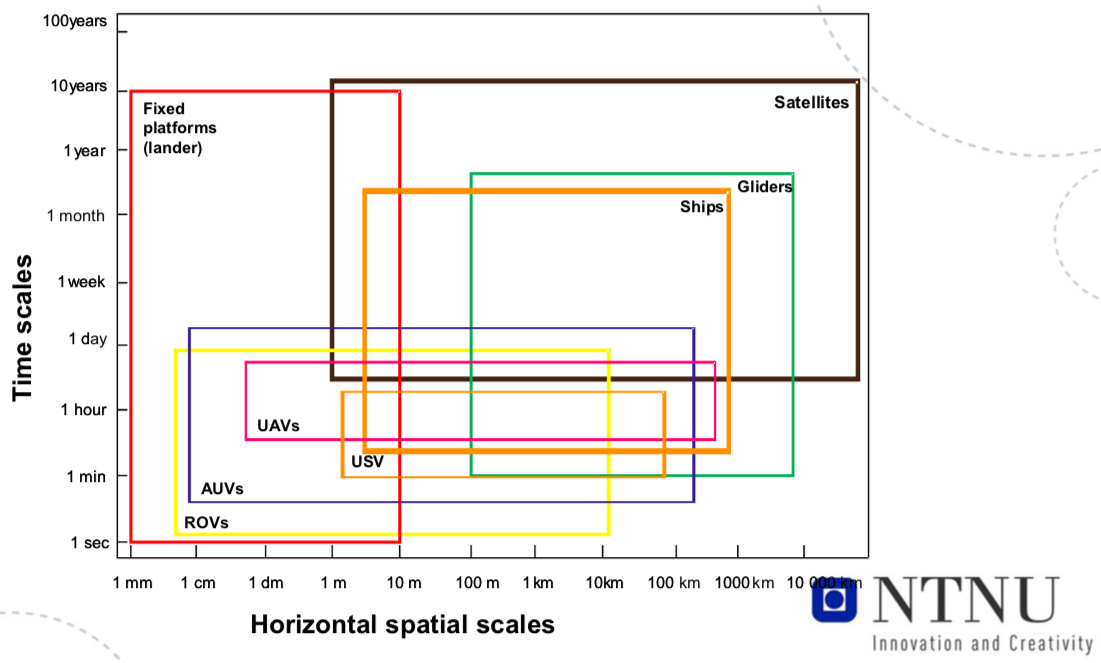
\includegraphics[width= 18cm]{Images/appendix/platforms.png}
    \caption{Sensor Platforms Temporal and Spatial Resolution and Coverage}
    \label{fig:platforms}
\end{figure}

\chapter{Experiment Set-Up}
\label{app:method}

\newpage
\begin{figure}[H]
  \newcommand*\FigVSkip{0.5em}
  \newcommand*\FigHSkip{0.1em}
  \newsavebox\FigBox
  \centering
  % Top image is centered, so no need to get width
 \sbox{\FigBox}{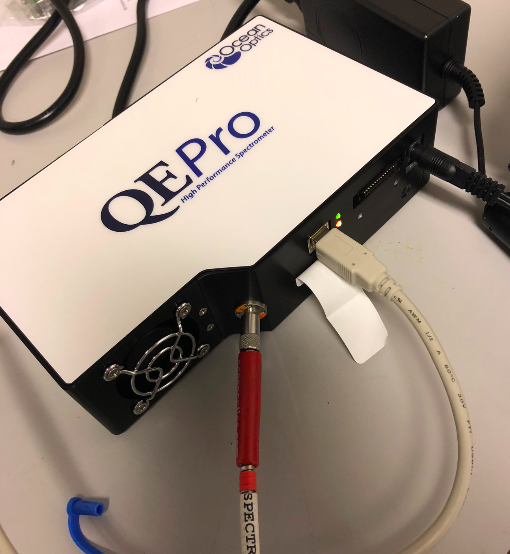
\includegraphics[height=5cm]{Images/method/qe-pro.png}}
  \begin{minipage}{\wd\FigBox}
    \centering\usebox{\FigBox}
    \subcaption{a) QE Pro}
  \end{minipage}
    % Top image is centered, so no need to get width
 \sbox{\FigBox}{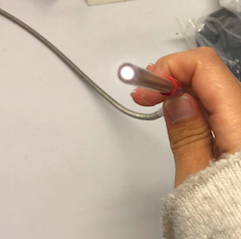
\includegraphics[height=5cm]{Images/method/light.png}}
  \begin{minipage}{\wd\FigBox}
    \centering\usebox{\FigBox}
    \subcaption{b) Reflection Probe}
  \end{minipage}
  % Save first image in a box to get the width
  \sbox{\FigBox}{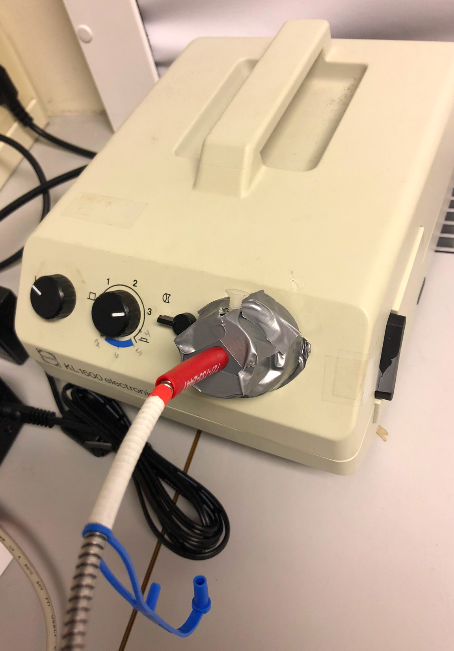
\includegraphics[height=5cm]{Images/method/lightsource.png}}
  \begin{minipage}{\wd\FigBox}
    \centering\usebox{\FigBox}
    \subcaption{c) Light Source, Schott KL1500, 150 W Halogen}
  \end{minipage}\hspace*{\FigHSkip}
  % Save second image 
\end{figure}

\begin{figure}[H]
  \newcommand*\FigVSkip{0.5em}
  \newcommand*\FigHSkip{0.1em}
  \newsavebox\FigBox
  \centering
  % Top image is centered, so no need to get width
 \sbox{\FigBox}{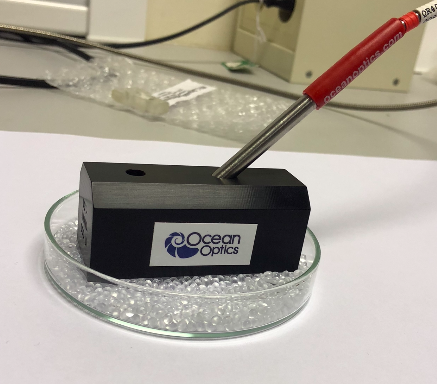
\includegraphics[height=4cm]{Images/method/setup.png}}
  \begin{minipage}{\wd\FigBox}
    \centering\usebox{\FigBox}
    \subcaption{d) Reflection Probe Holder from Ocean Optics}
  \end{minipage}
    % Top image is centered, so no need to get width
 \sbox{\FigBox}{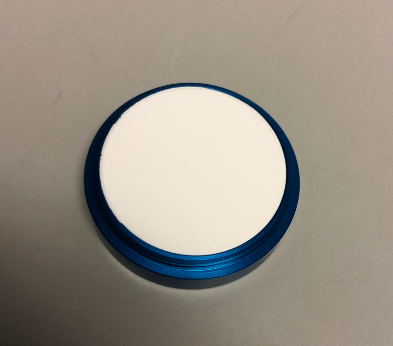
\includegraphics[height=4cm]{Images/method/lamber.png}}
  \begin{minipage}{\wd\FigBox}
    \centering\usebox{\FigBox}
    \subcaption{e) WS-1 Reflectance Standard, Lambertian Surface from Ocean Optics}
  \end{minipage}
  % Save first image in a box to get the width
  \sbox{\FigBox}{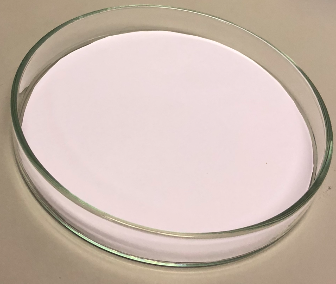
\includegraphics[height=4cm]{Images/appendix/papir.png}}
  \begin{minipage}{\wd\FigBox}
    \centering\usebox{\FigBox}
    \subcaption{f) Paper Background}
  \end{minipage}\hspace*{\FigHSkip}
  % Save second image 
  \caption{The Laboratory Set-up}
  \label{fig:lab-set-up}
\end{figure}


\chapter{PCA Results}
\label{app:PCA_res_full}
%FULL SET
\section{Full Set}
\begin{figure}[H]
    \centering
    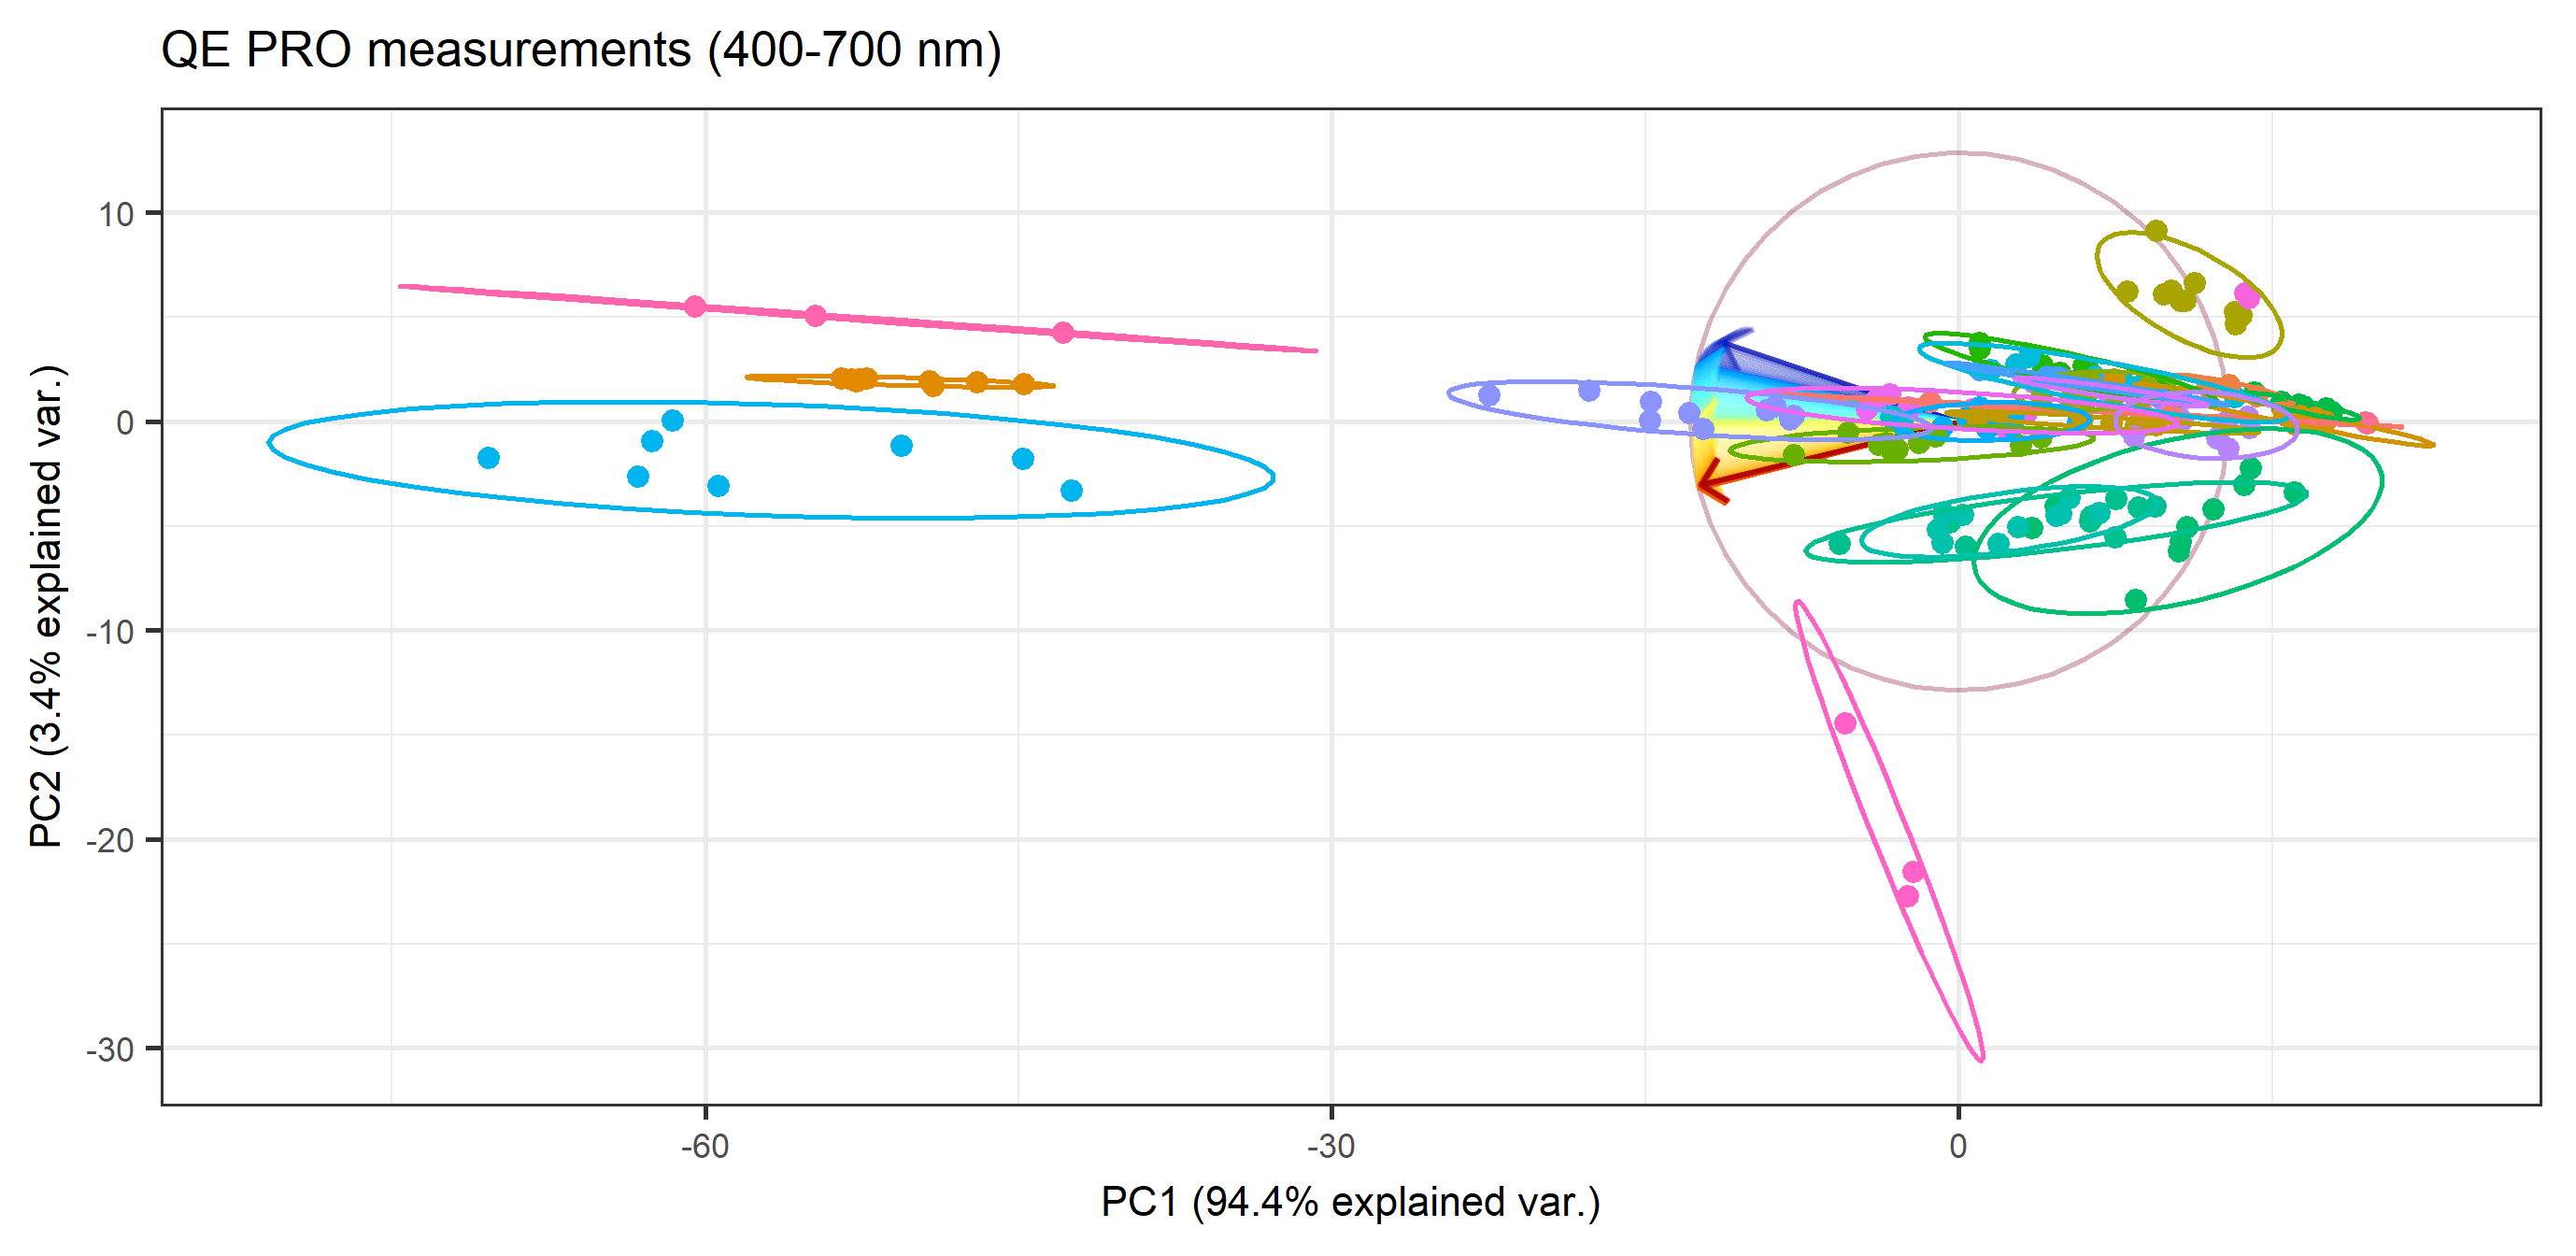
\includegraphics[width=1\textwidth]{Images/results/PCA_plastics_full_only_scat.png}
    \caption{Scatter plot of the results of the PCA with all plastic samples}
    \label{fig:PCA_plastics_only_full_scat}
\end{figure}

\begin{figure}[H]
   \centering
    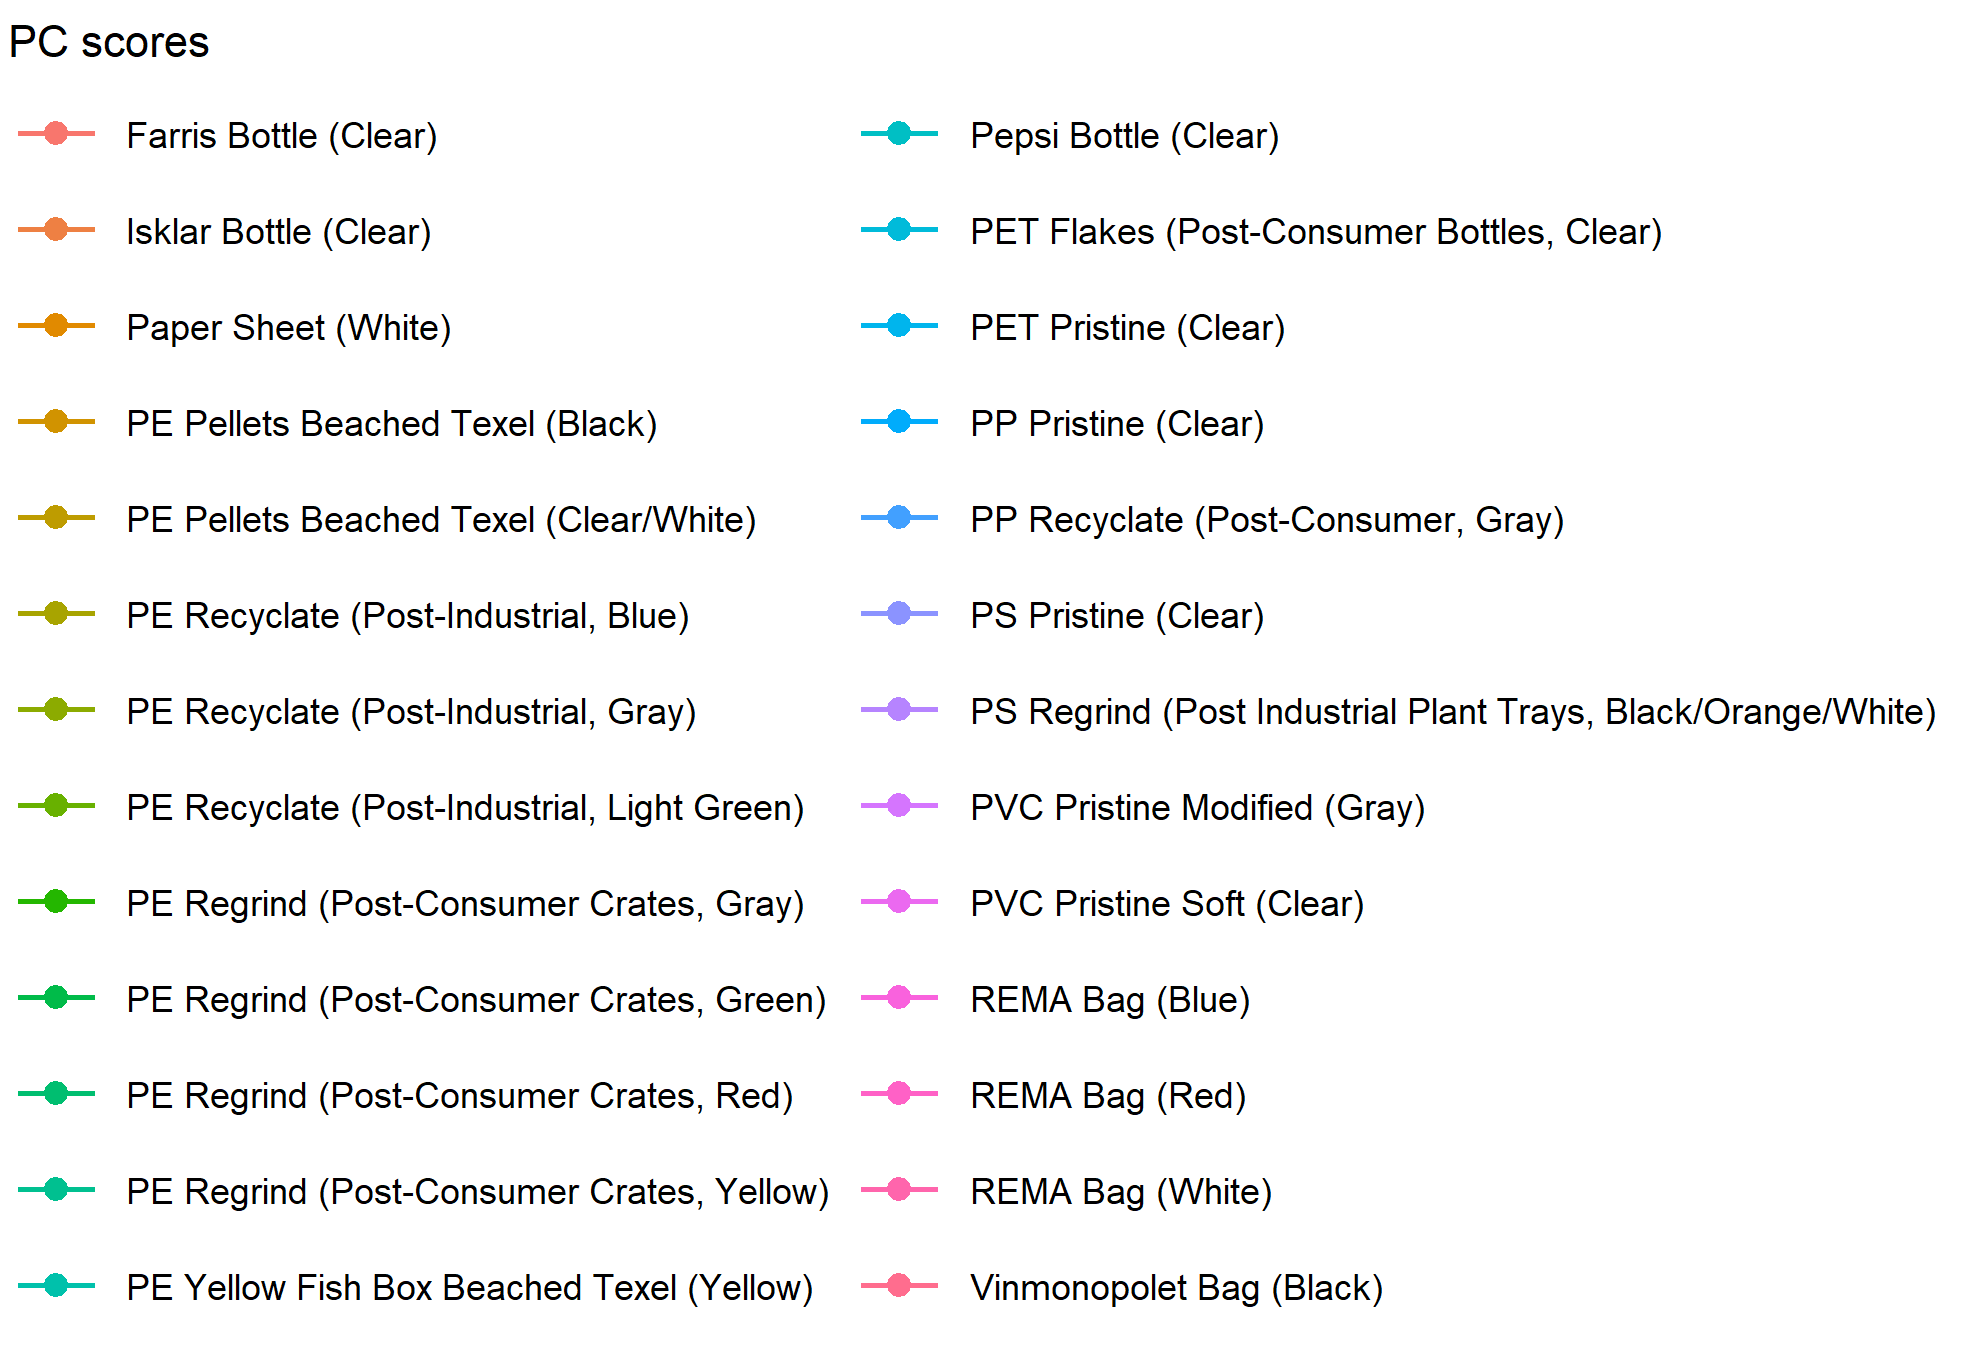
\includegraphics[width=0.7\textwidth]{Images/results/PCA_plastics_full_list.png}
  \caption{List of all scanned plastic samples and their respective colors.}
  \label{fig:PCA_plastics_full_list}
\end{figure}

\begin{figure}[H]
    \centering
    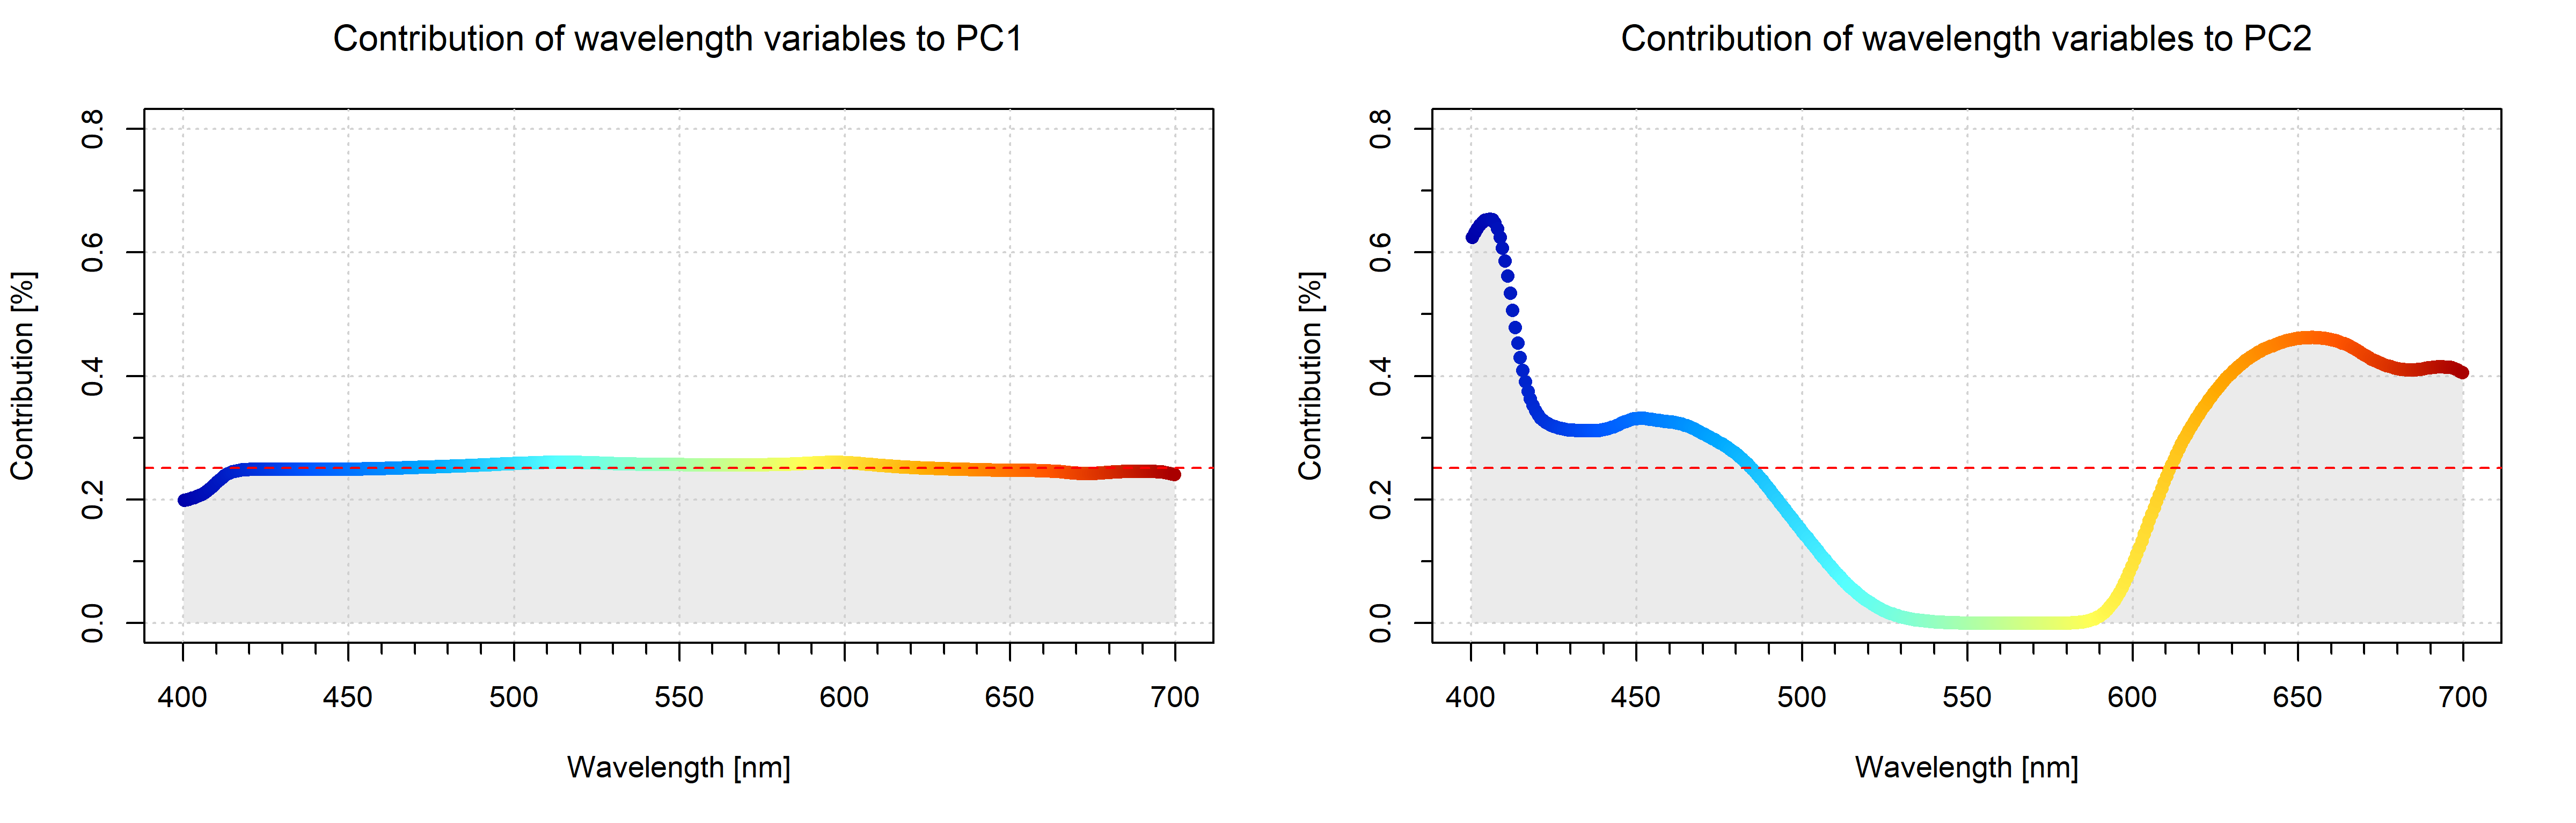
\includegraphics[width=1\textwidth]{Images/results/PCA_plastics_full_doub_cont.png}
    \caption{Contribution plot of the results of the PCA with all plastic samples.}
    \label{fig:PCA_plastics_full_doub_cont}
\end{figure}

%REDUCED SET
\section{Reduced Set}
\begin{figure}[H]
    \centering
    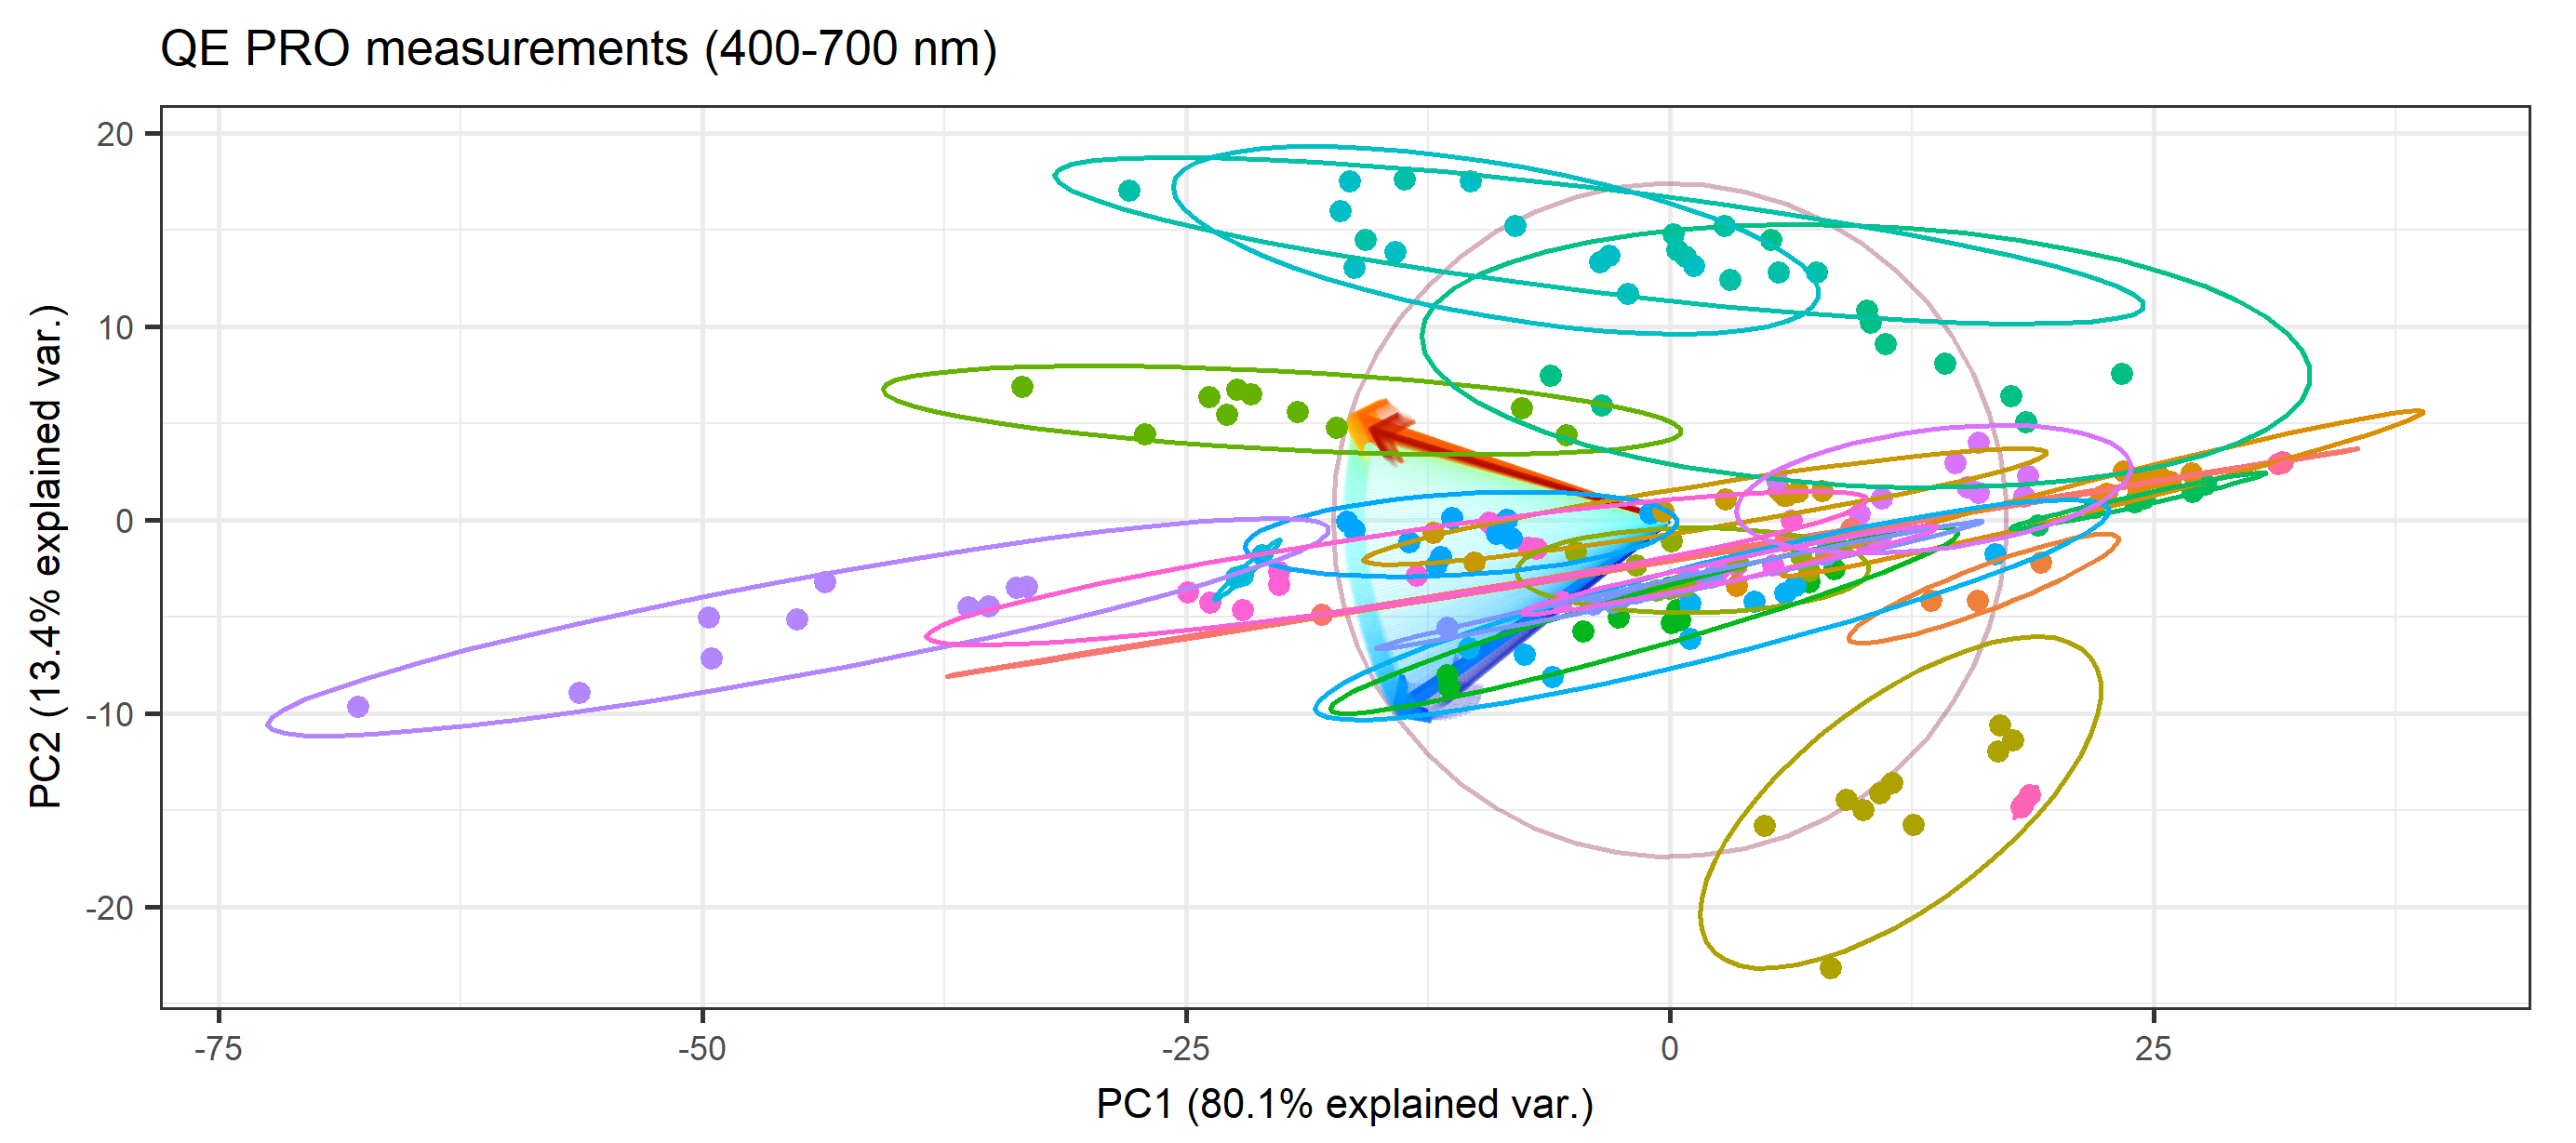
\includegraphics[width=1\textwidth]{Images/results/PCA_plastics_reduced_only_scat.png}
    \caption{Results of the PCA with reduced Plastic Samples}
    \label{fig:PCA_plastics_reduced_only_scat}
\end{figure}

\begin{figure}[H]
    \centering
    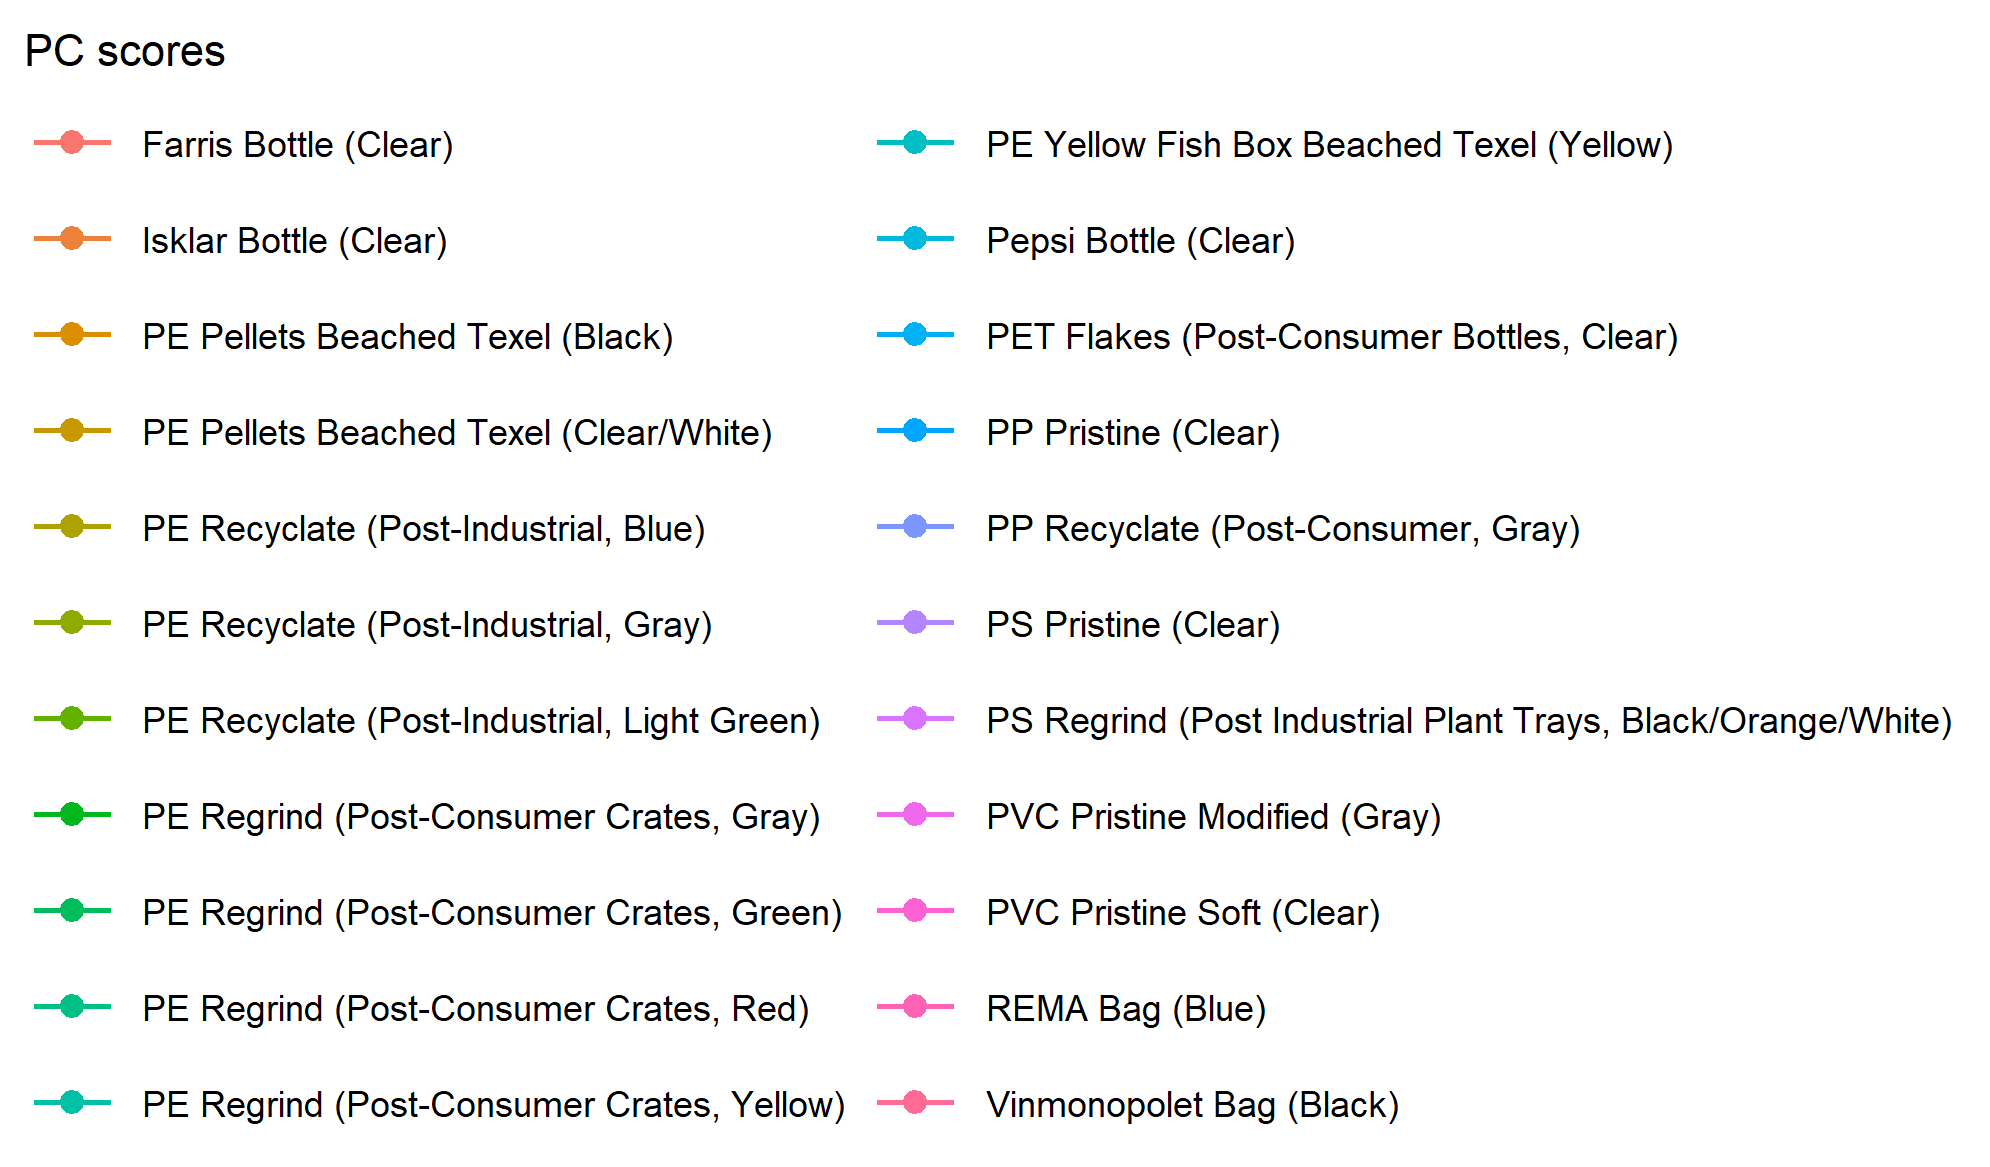
\includegraphics[width=0.7\textwidth]{Images/results/PCA_plastics_reduced_list.png}
    \caption{List of the reduced scanned plastic samples and their respective colors.}
    \label{fig:PCA_plastics_reduced_list}
\end{figure}

\begin{figure}[H]
    \centering
    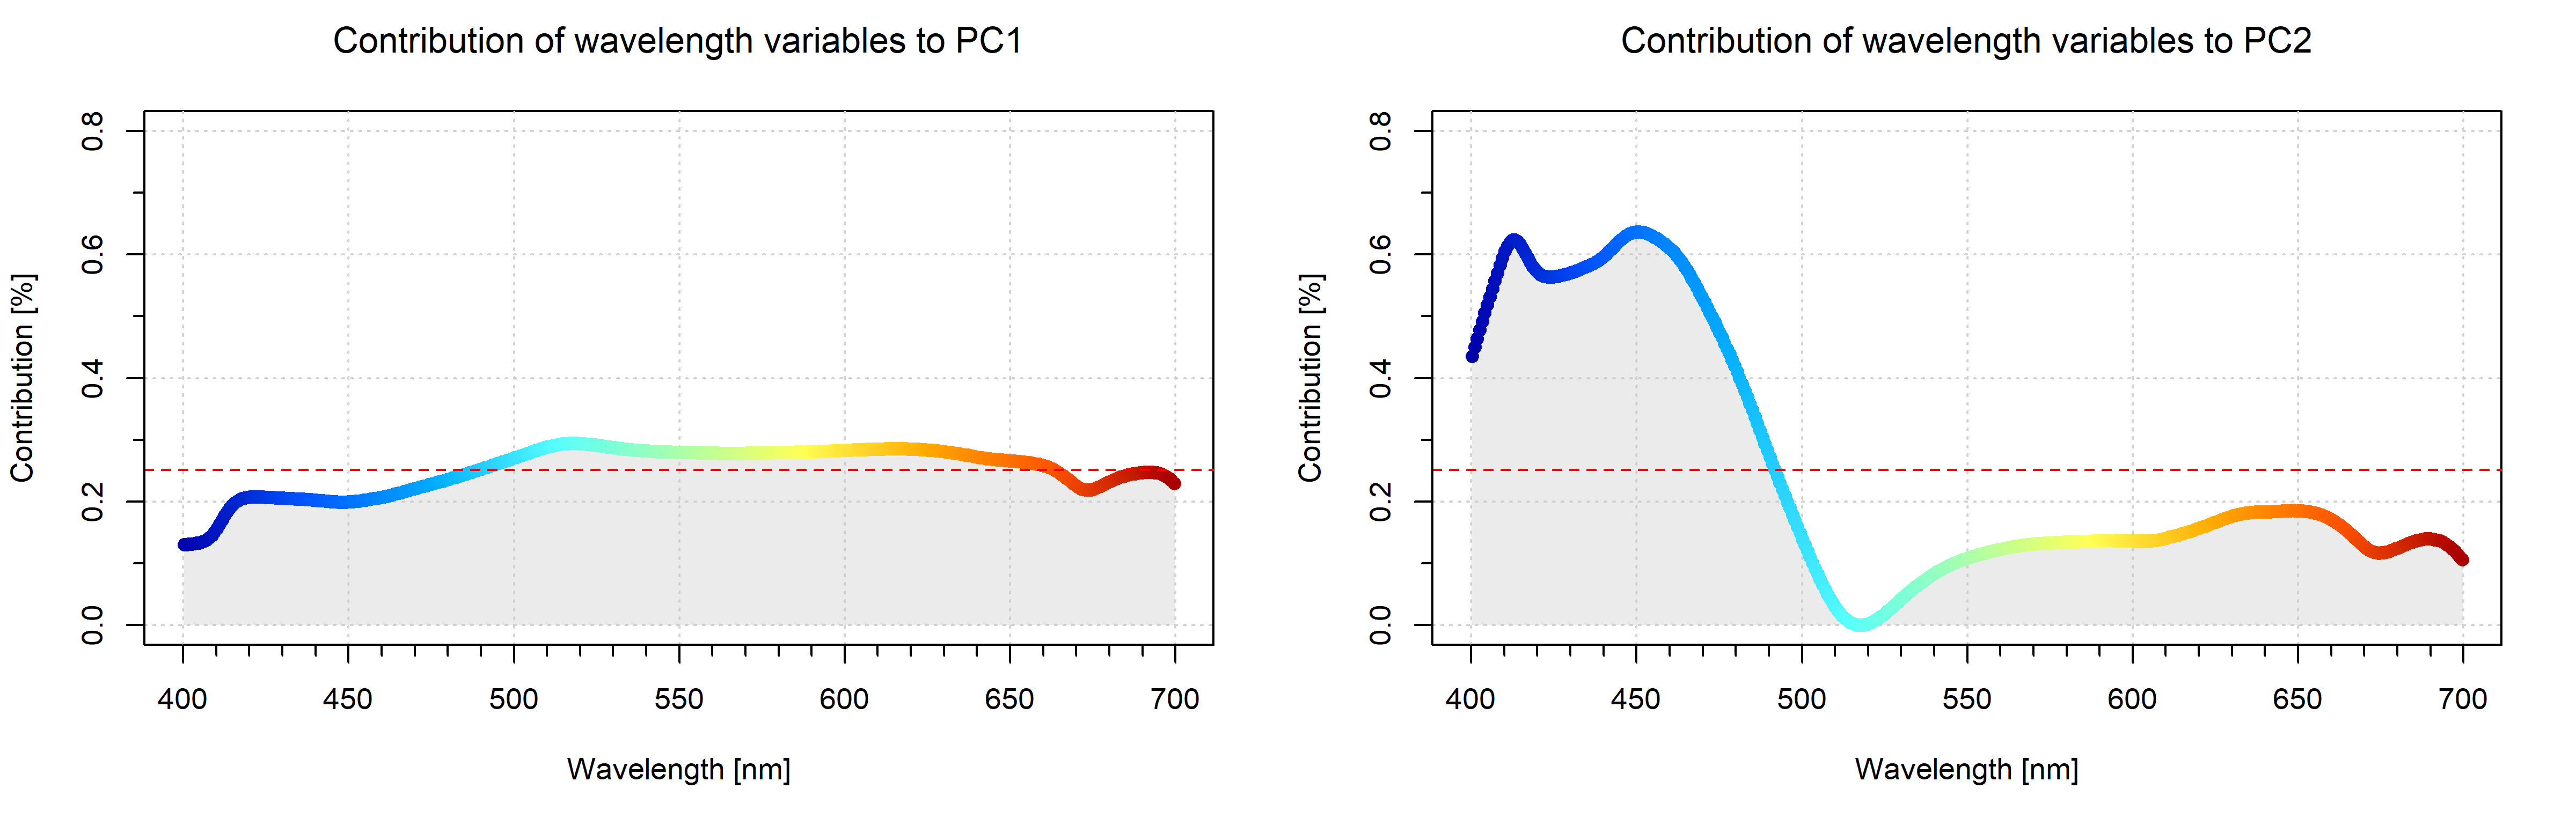
\includegraphics[width=1\textwidth]{Images/results/PCA_plastics_reduced_doub_cont.png}
    \caption{Contribution plots of the two principal components of the PCA with reduced plastic samples}
    \label{fig:PCA_plastics_doub_cont}
\end{figure}

%BIO
\section{Plastics an Biological Components}
\begin{figure}[H]
    \centering
    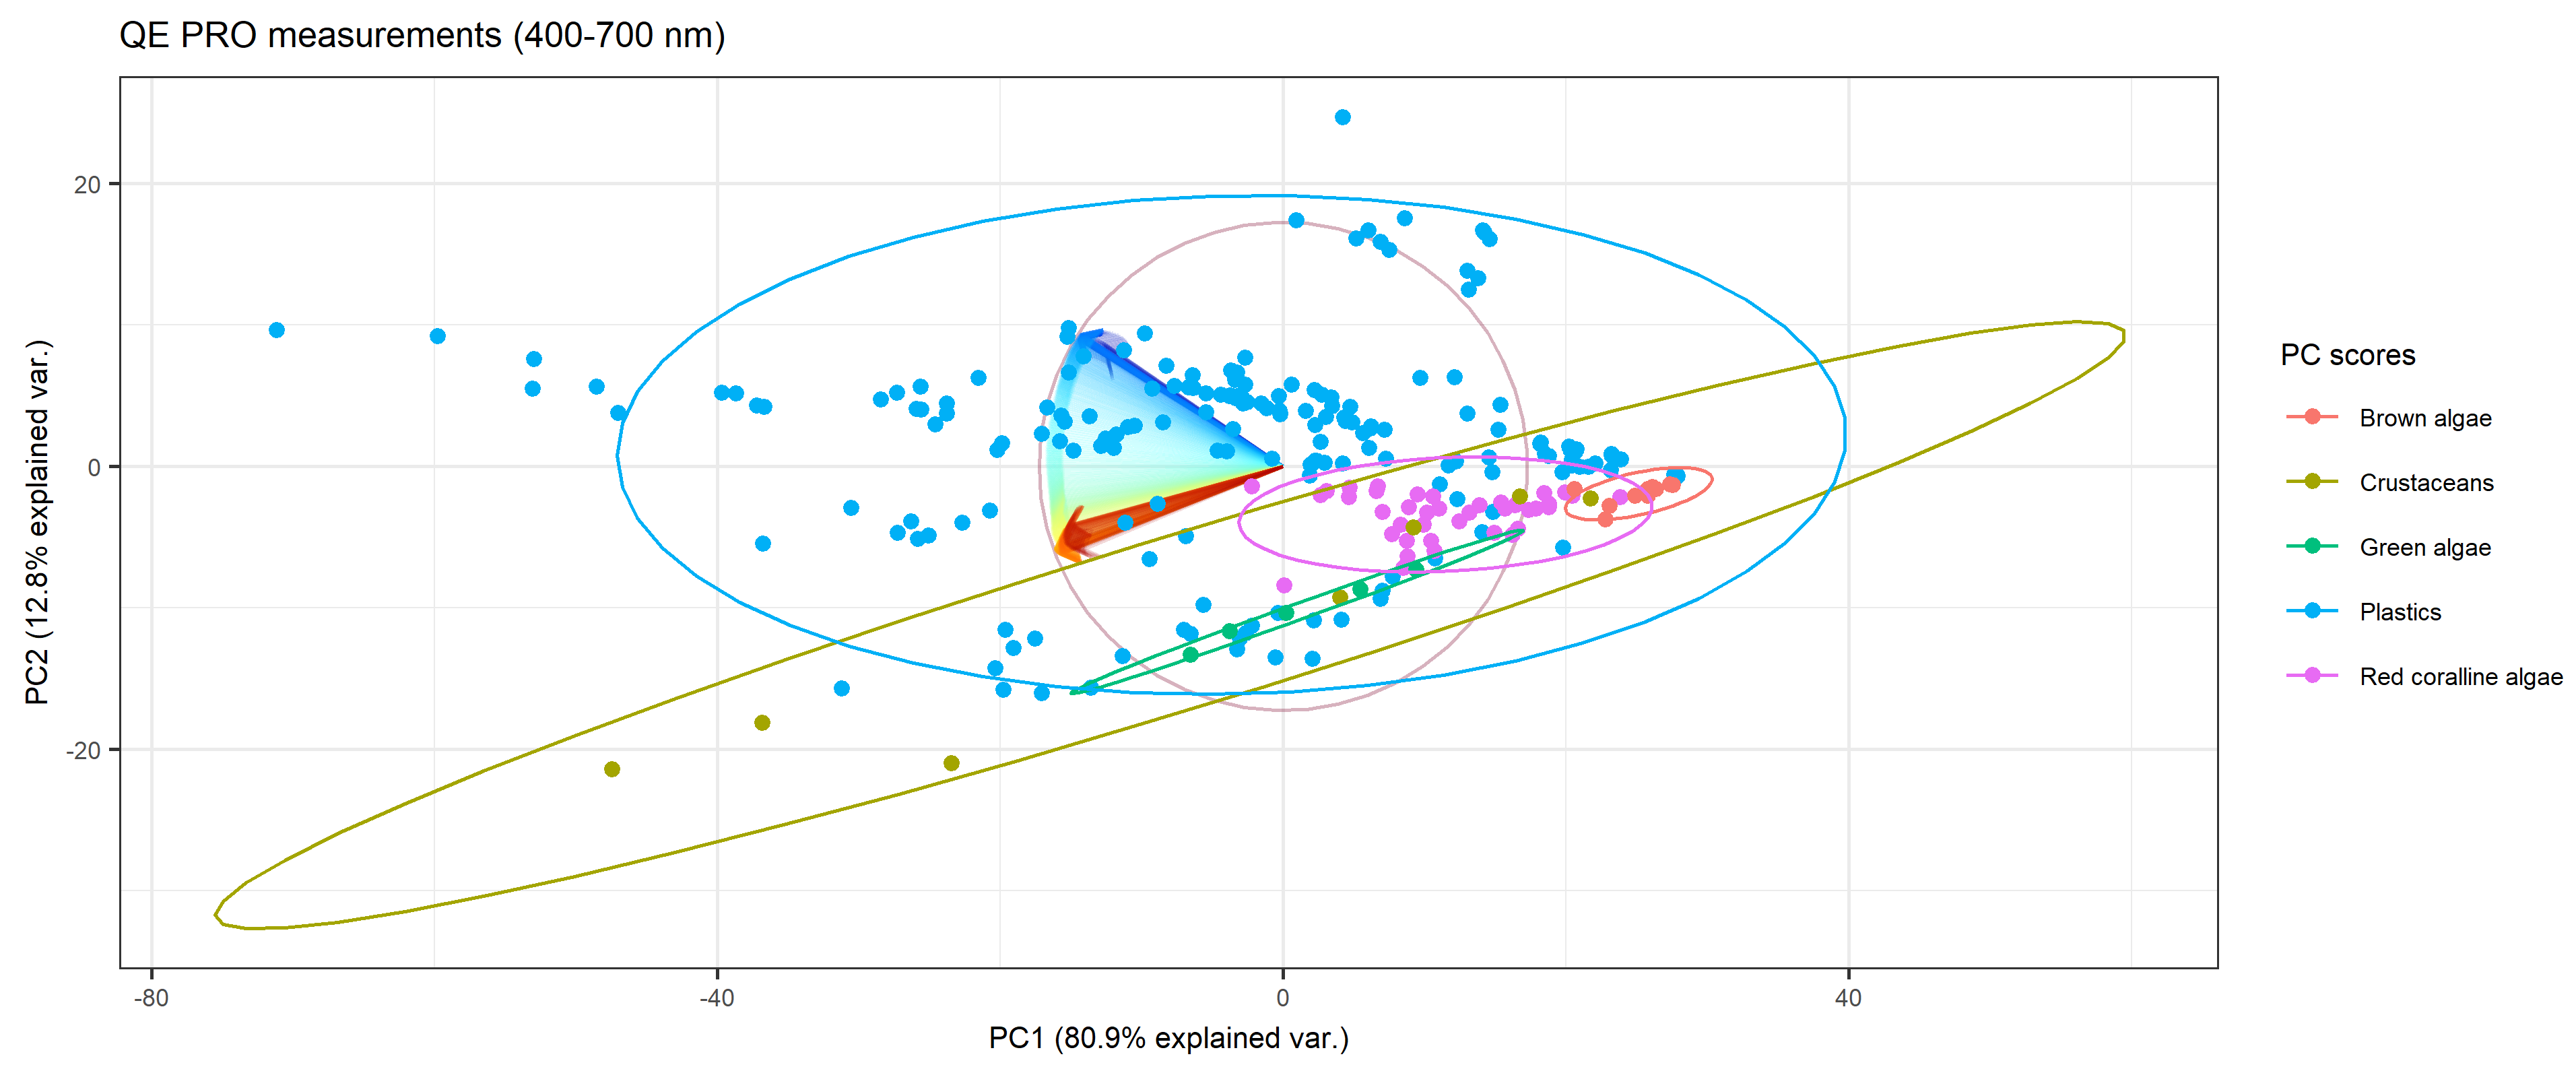
\includegraphics[width=1\textwidth]{Images/results/PCA_plastics_and_biology_scat_clust.png}
    \caption{Results of the PCA with Plastics and Biological Components}
    \label{fig:PCA_plastics_and_biology_scat}
\end{figure}


\begin{figure}[H]
  \newcommand*\FigVSkip{0.5em}
  \newcommand*\FigHSkip{0.1em}
  \newsavebox\FigBox
  \centering
  % Top image is centered, so no need to get width
 \sbox{\FigBox}{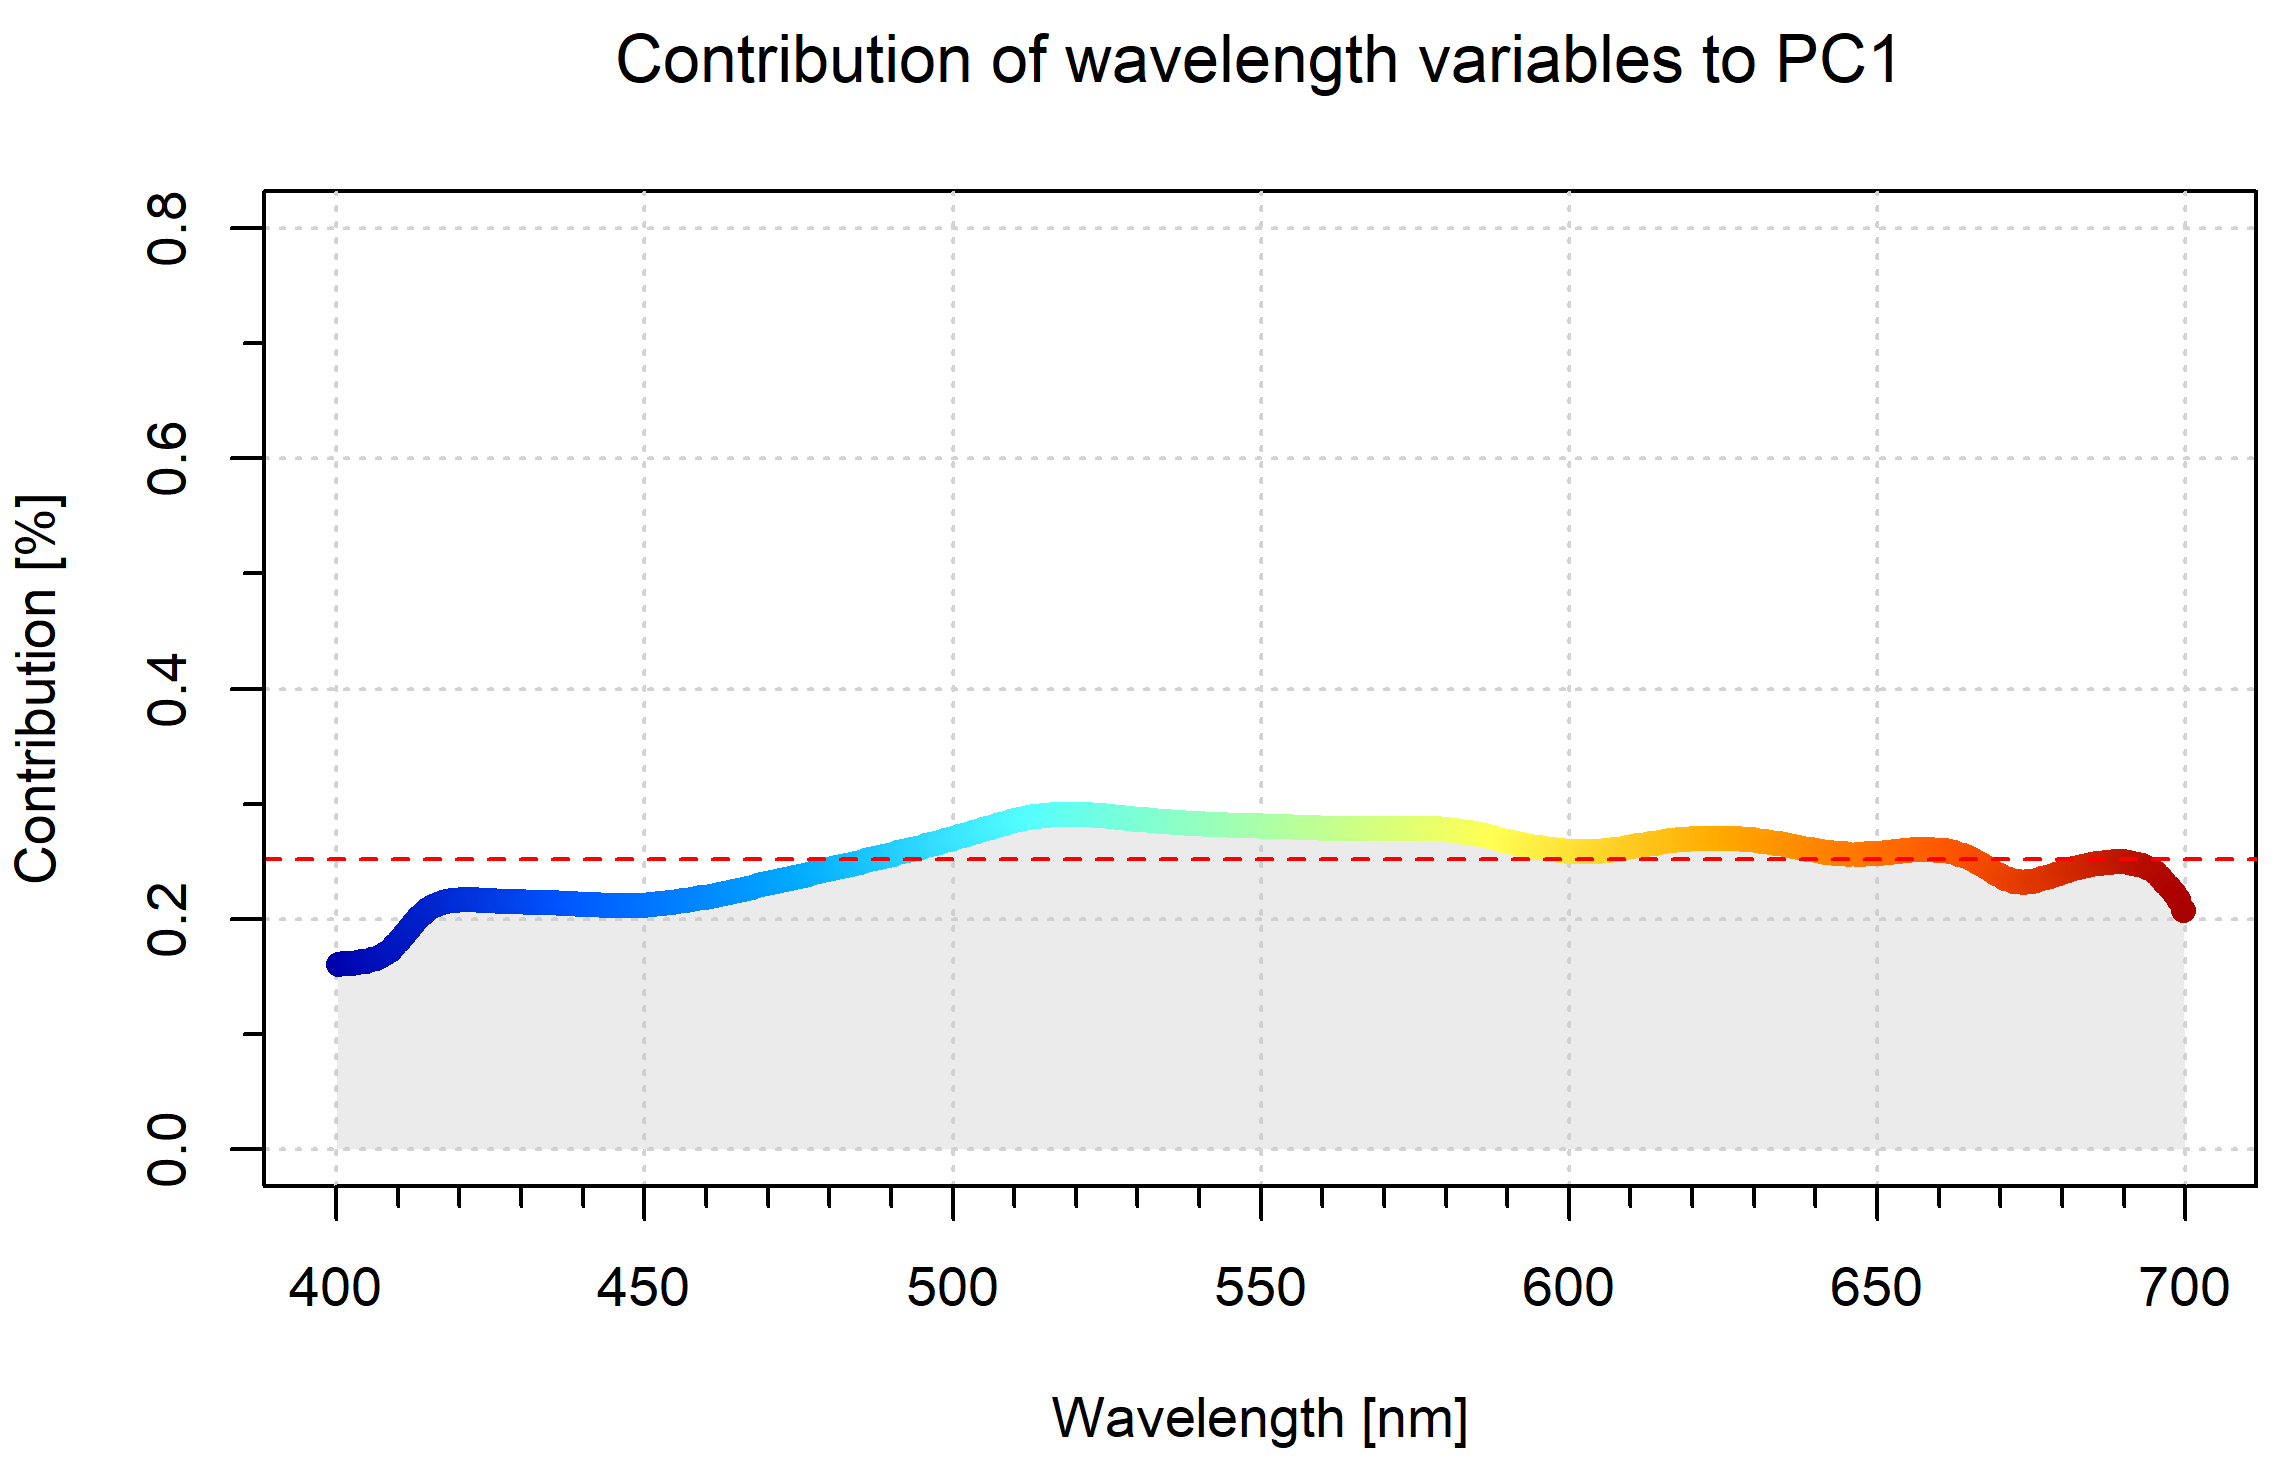
\includegraphics[scale=0.56]{Images/results/PCA_plastics_and_biology_cont_pc1.png}}
  \begin{minipage}{\wd\FigBox}
    \centering\usebox{\FigBox}
     \label{fig:PCA_plastics_and_biology_cont_pc1}
  \end{minipage}
    % Top image is centered, so no need to get width
 \sbox{\FigBox}{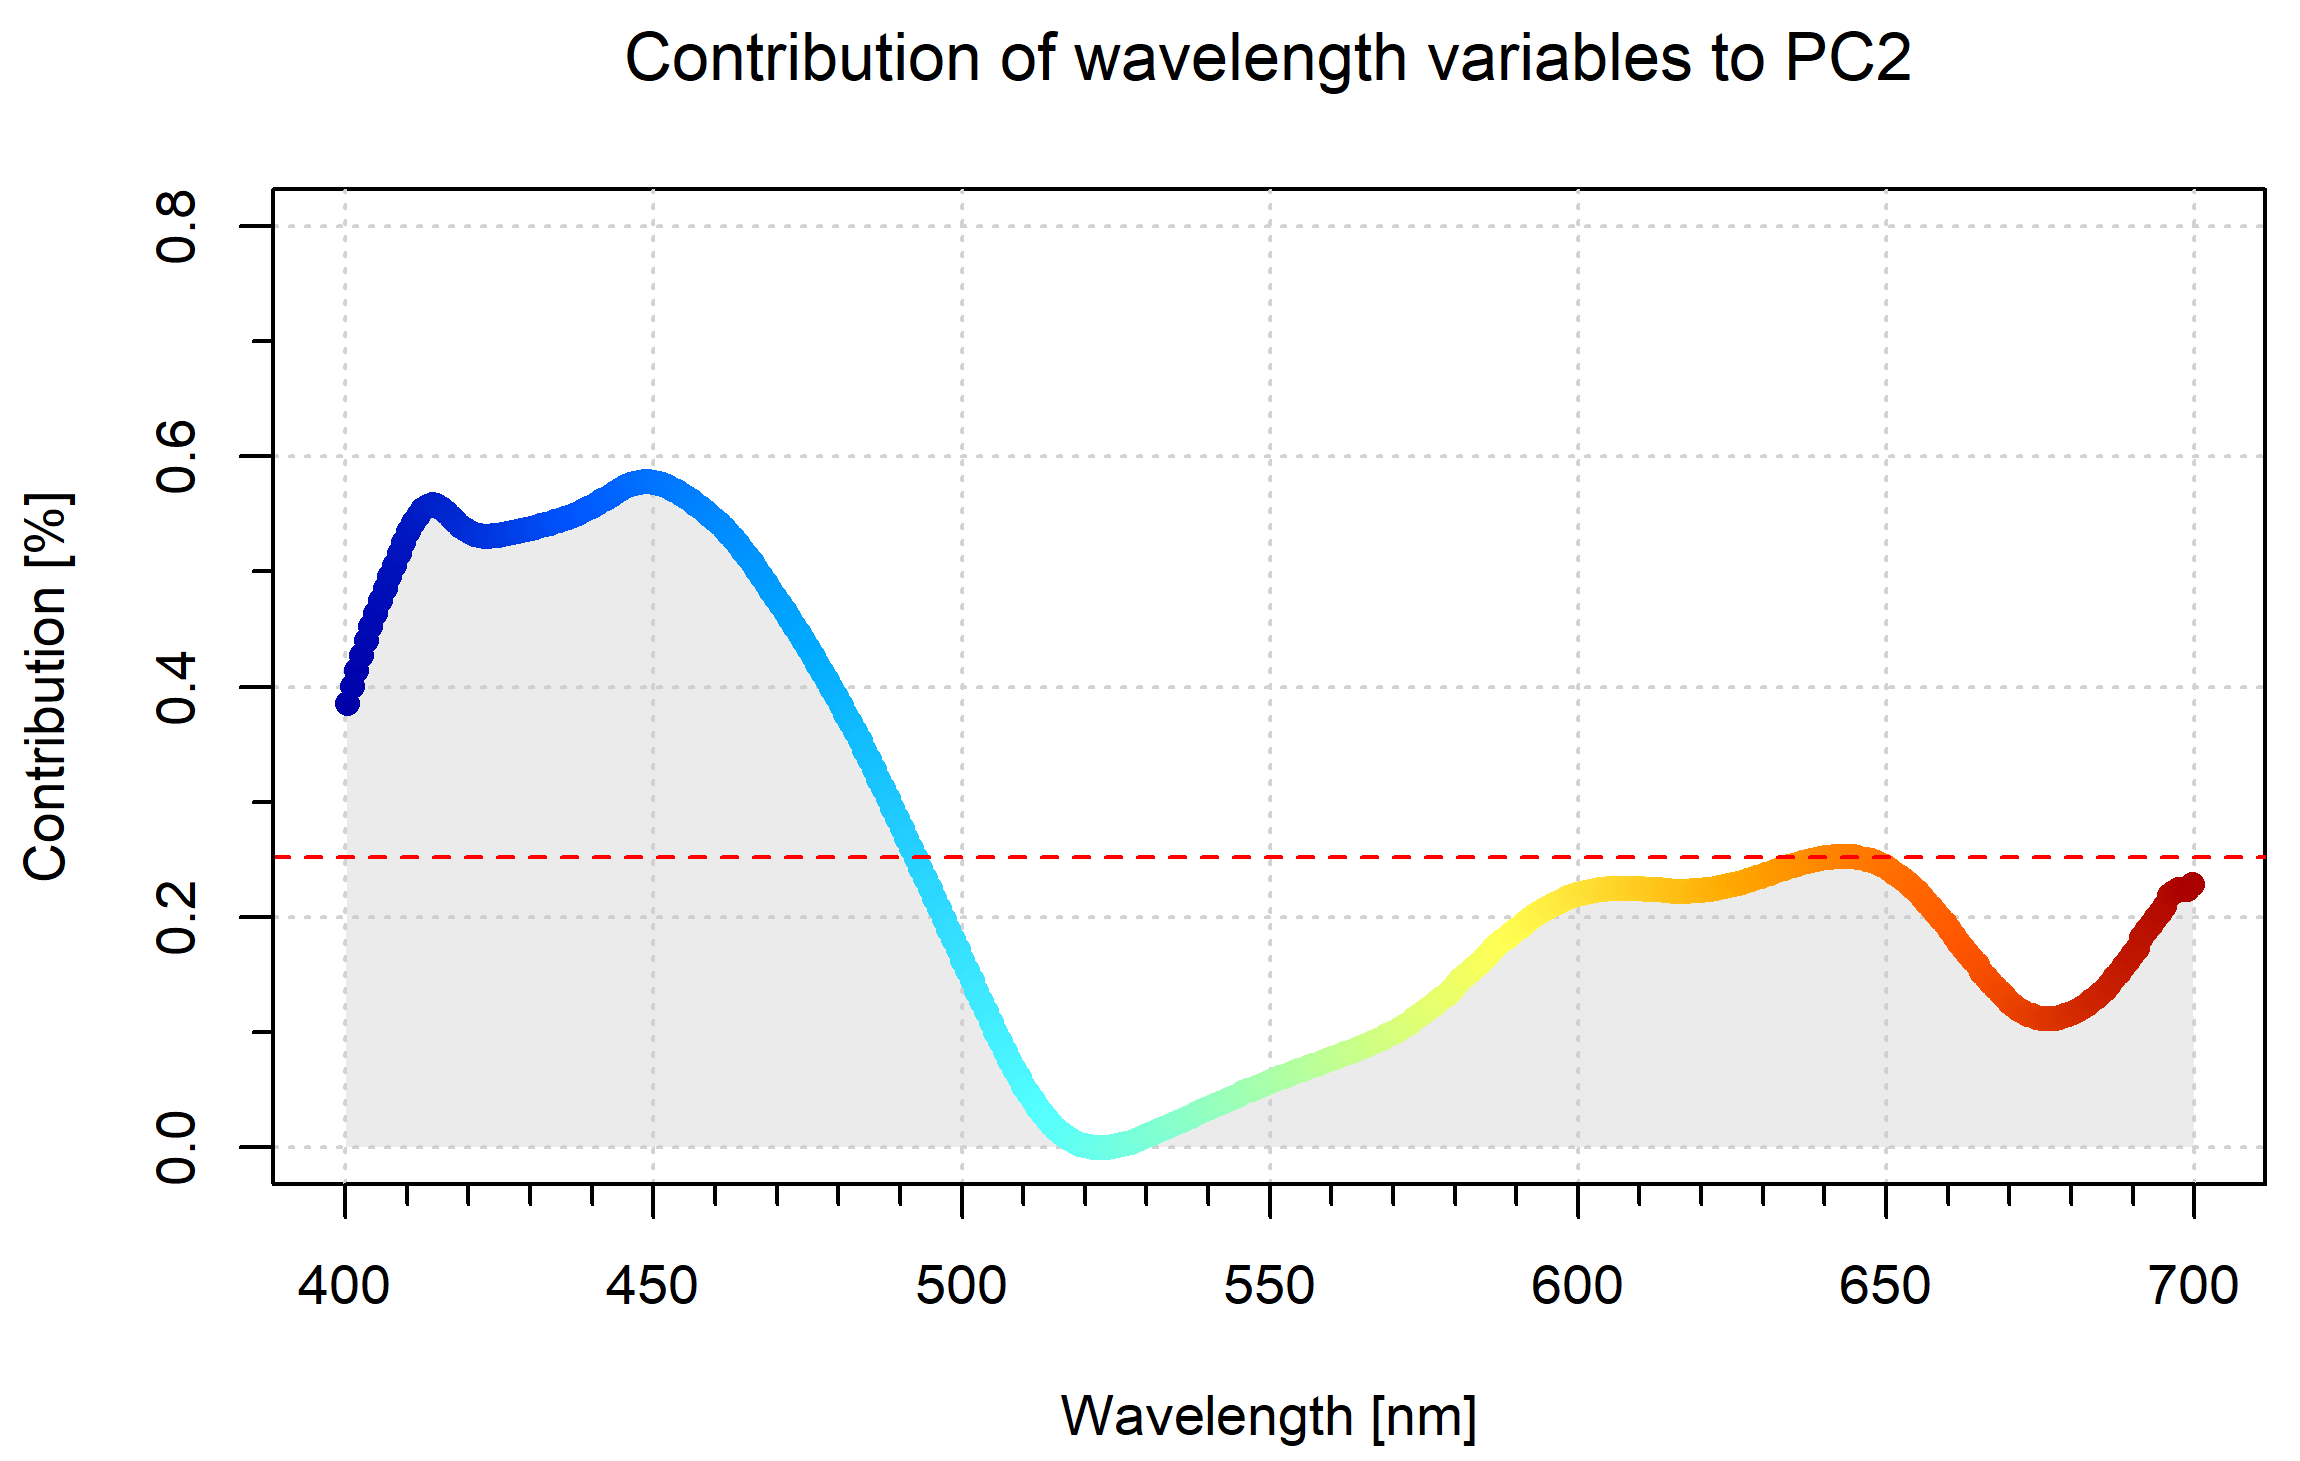
\includegraphics[scale=0.56]{Images/results/PCA_plastics_and_biology_cont_pc2.png}}
  \begin{minipage}{\wd\FigBox}
    \centering\usebox{\FigBox}
  \label{fig:PCA_plastics_and_biology_cont_pc2}
  \end{minipage}
  % Save second image 
  \caption{Contribution plots for the PCA with plastic and biological samples}
\label{fig:PCA_and_bio_cont_plots}
\end{figure}





\chapter{List of Tested Plastic}
\label{app:list_plast}

\begin{figure}
    \centering
    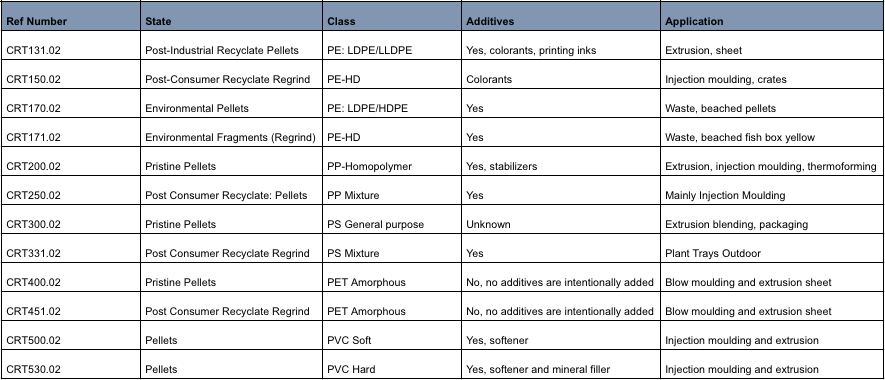
\includegraphics[height = 9cm, angle = 90]{Images/order.png}
    \caption{List of microplastics - state, class, additives and application}
    \label{fig:order}
\end{figure}

\begin{comment}
\begin{center}
\begin{adjustbox}{angle=90}
\begin{tabular}{ |c|l|l|l|l| } 
 \hline
 \textbf{Ref Number} & \textbf{State} & \textbf{Class} & \textbf{Additives} & \textbf{Application}\\ 
 \hline
CRT131.00 & Post-Industrial Recyclate Pellets & PE: LDPE/LLDPE & Colorants, Printing inks & Extrusion, sheet\\
CRT150.00 & Post-Consumer Recyclate Regrind & PE-HD & Colorants & Injection moulding, crates\\
CRT170.00 & Environmental Pellets & PE: LDPE/HDPE & Unspecified Additives & Waste, beached pellets\\
CRT171.00 & Environmental Fragments (Regrind) & PE-HD & Unspecified Additives & Waste, beached fish box yellow\\
CRT200.00 & Pristine Pellets & PP-Homopolymer & Stabilizers & Extrusion, injection moulding\\
CRT250.00 & Post Consumer Recyclate: Pellets & PP Mixture & Unspecified Additives & Mainly Injection Moulding\\
CRT300.00 & Pristine Pellets & PS General purpose & Unknown & Extrusion blending, packaging\\
CRT331.00 & Post Consumer Recyclate Regrind & PS Mixture & Unspecified Additives & Plant Trays Outdoor\\ 
CRT400.00 & Pristine Pellets & PET Amorphous & No intentionally additives & Blow moulding \& extrusion sheet\\
CRT451.00 & Post Consumer Recyclate Regrind & PET Amorphous & No intentionally additives & Blow moulding \& extrusion sheet\\
CRT500.00 & Pellets & PVC Soft & Softener & Injection moulding \& extrusion\\
CRT530.00 & Pellets & PVC Hard & Softener \& Mineral Filler & Injection moulding \& extrusion\\
 \hline
\end{tabular}
\end{adjustbox}
\end{center}
\end{comment}

\chapter{Images of Tested Plastic Samples}
\label{app:image_plast}

\begin{figure}
    \centering
    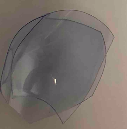
\includegraphics[width = 8cm]{Images/appendix/farris.png}
    \caption{Farris, Clear but slightly Blue}
    \label{fig:my_label}
\end{figure}

\begin{figure}
    \centering
    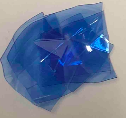
\includegraphics[width = 8cm]{Images/appendix/isklar.png}
    \caption{Isklar, Blue}
    \label{fig:isklar}
\end{figure}

\begin{figure}
    \centering
    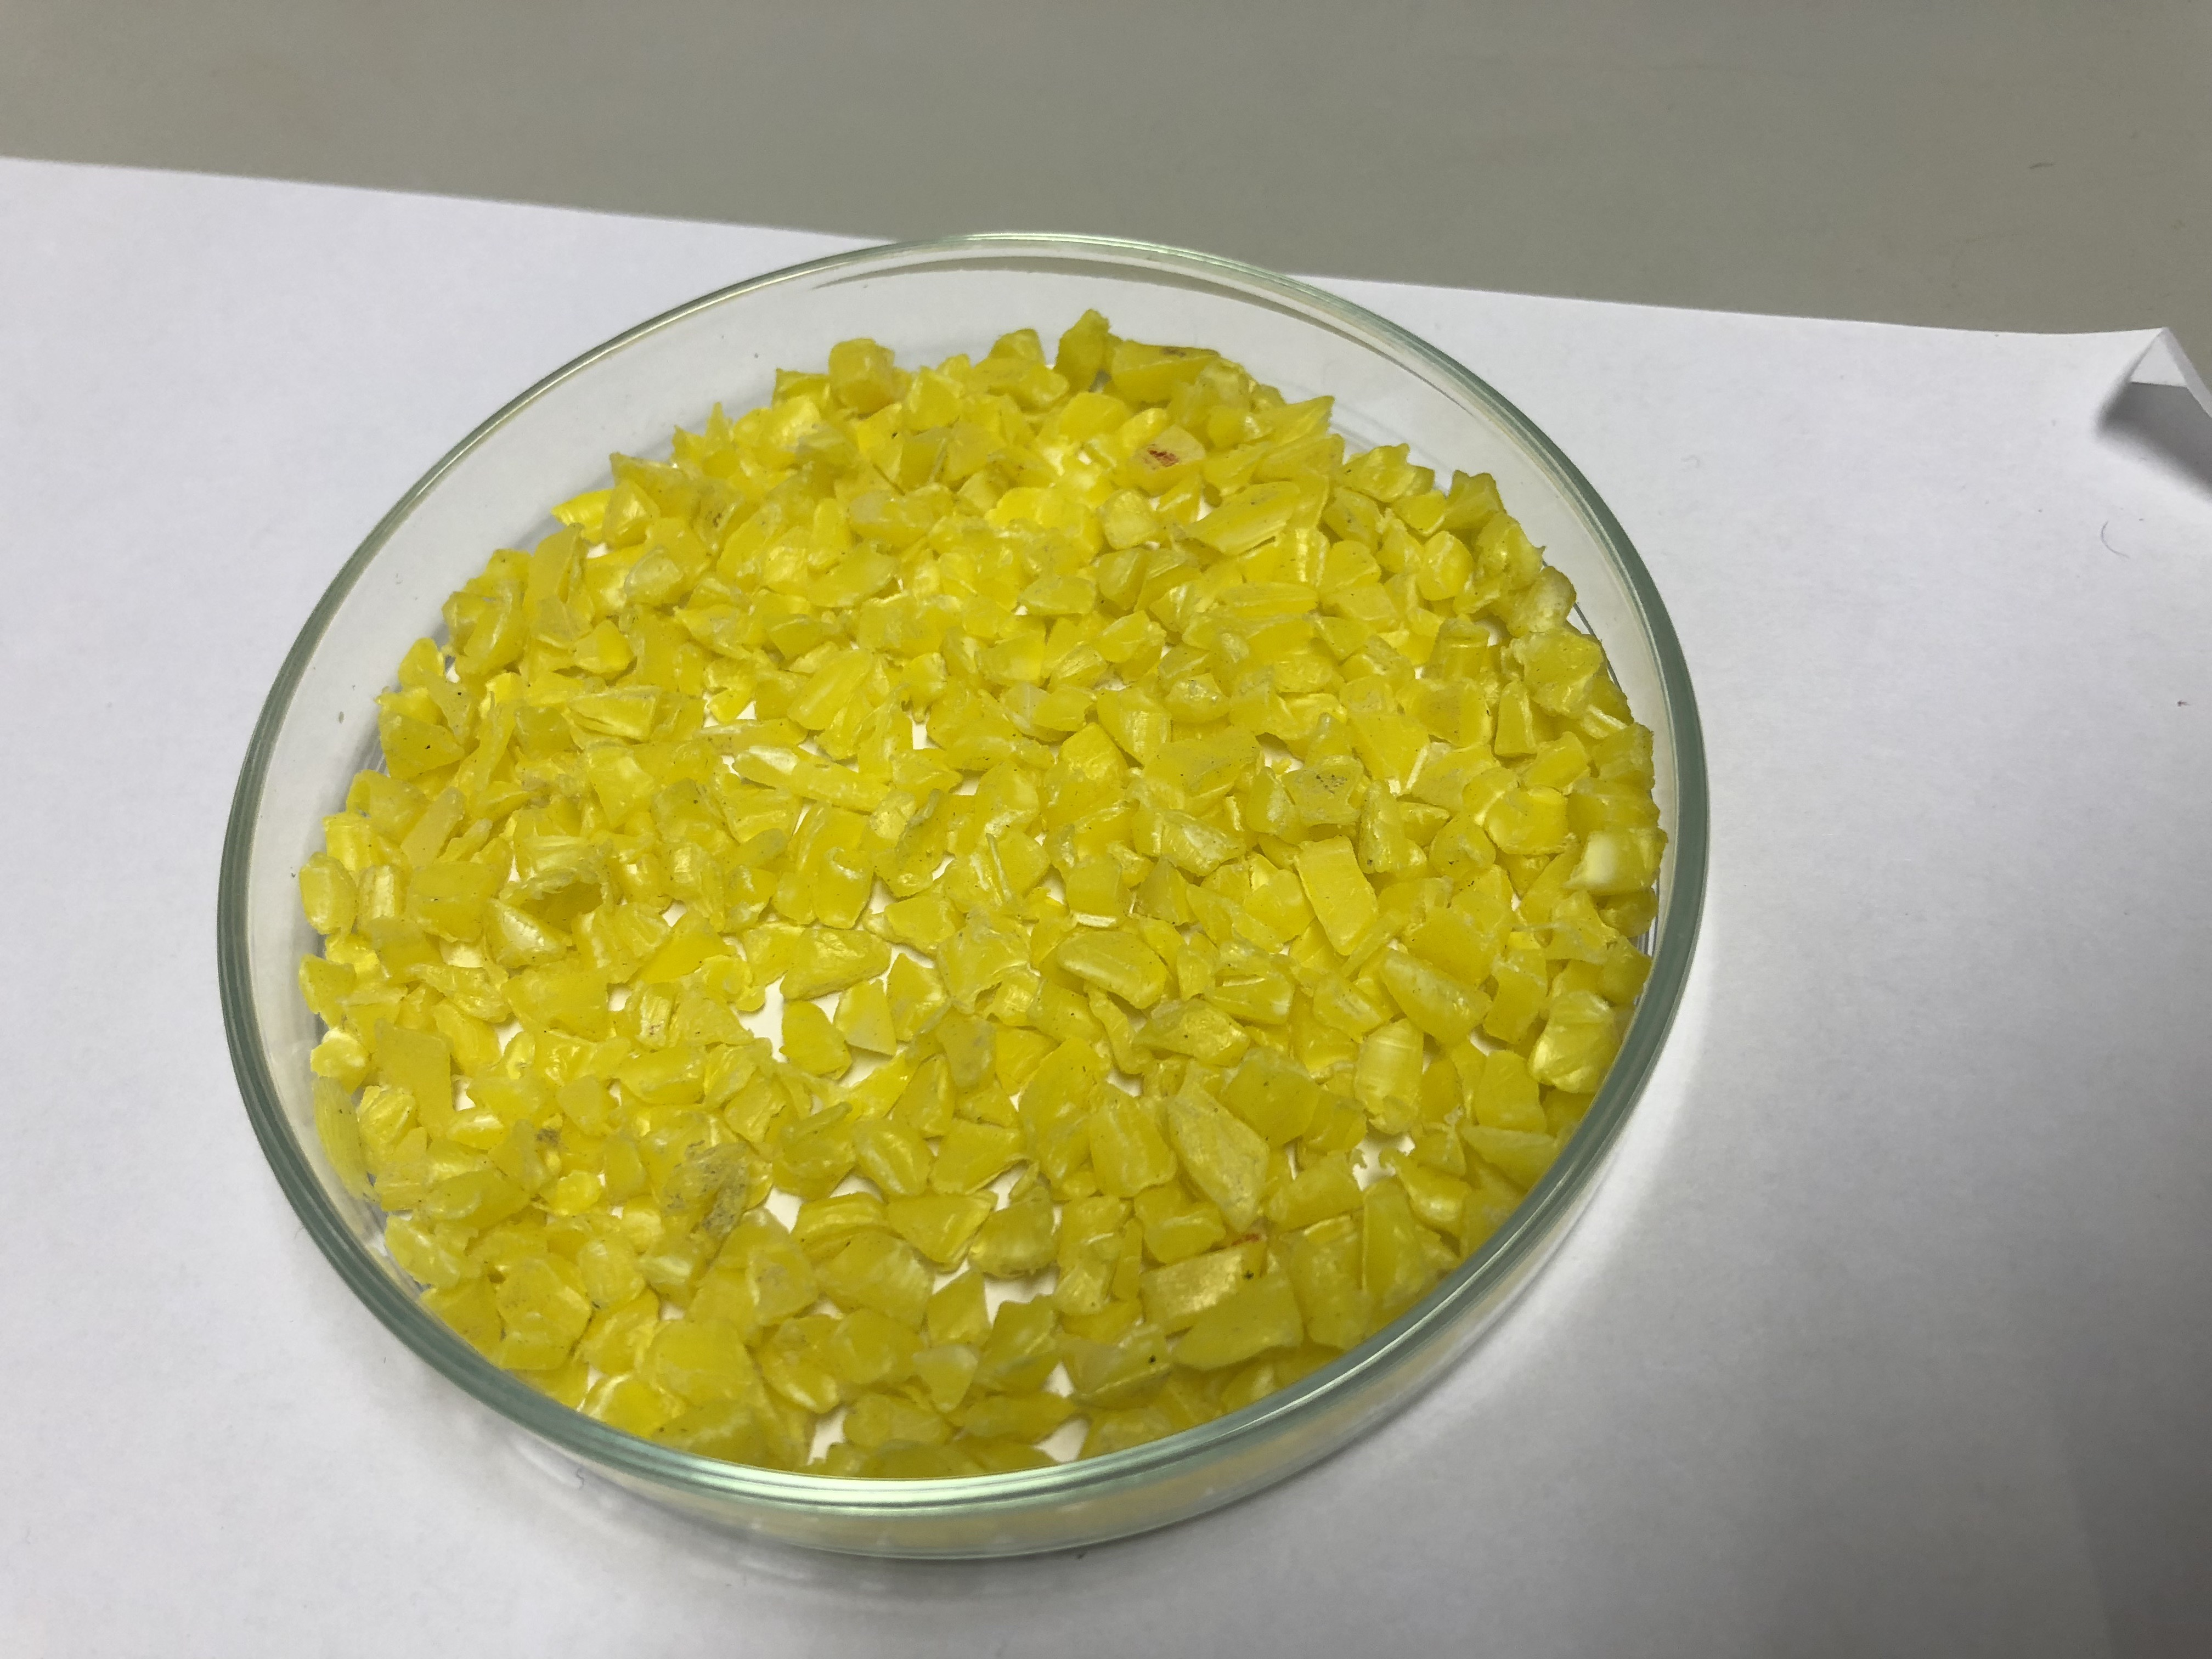
\includegraphics[width = 12cm]{Images/appendix/PE-Yellow-Fish-Box-Beached-Texel.jpg}
    \caption{PE environmental, yellow fish box}
    \label{fig:pe_env}
\end{figure}


\begin{figure}
    \centering
    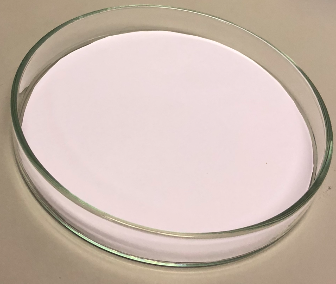
\includegraphics[width = 12cm]{Images/appendix/papir.png}
    \caption{Paper sheet}
    \label{fig:paper}
\end{figure}

\begin{figure}
    \centering
    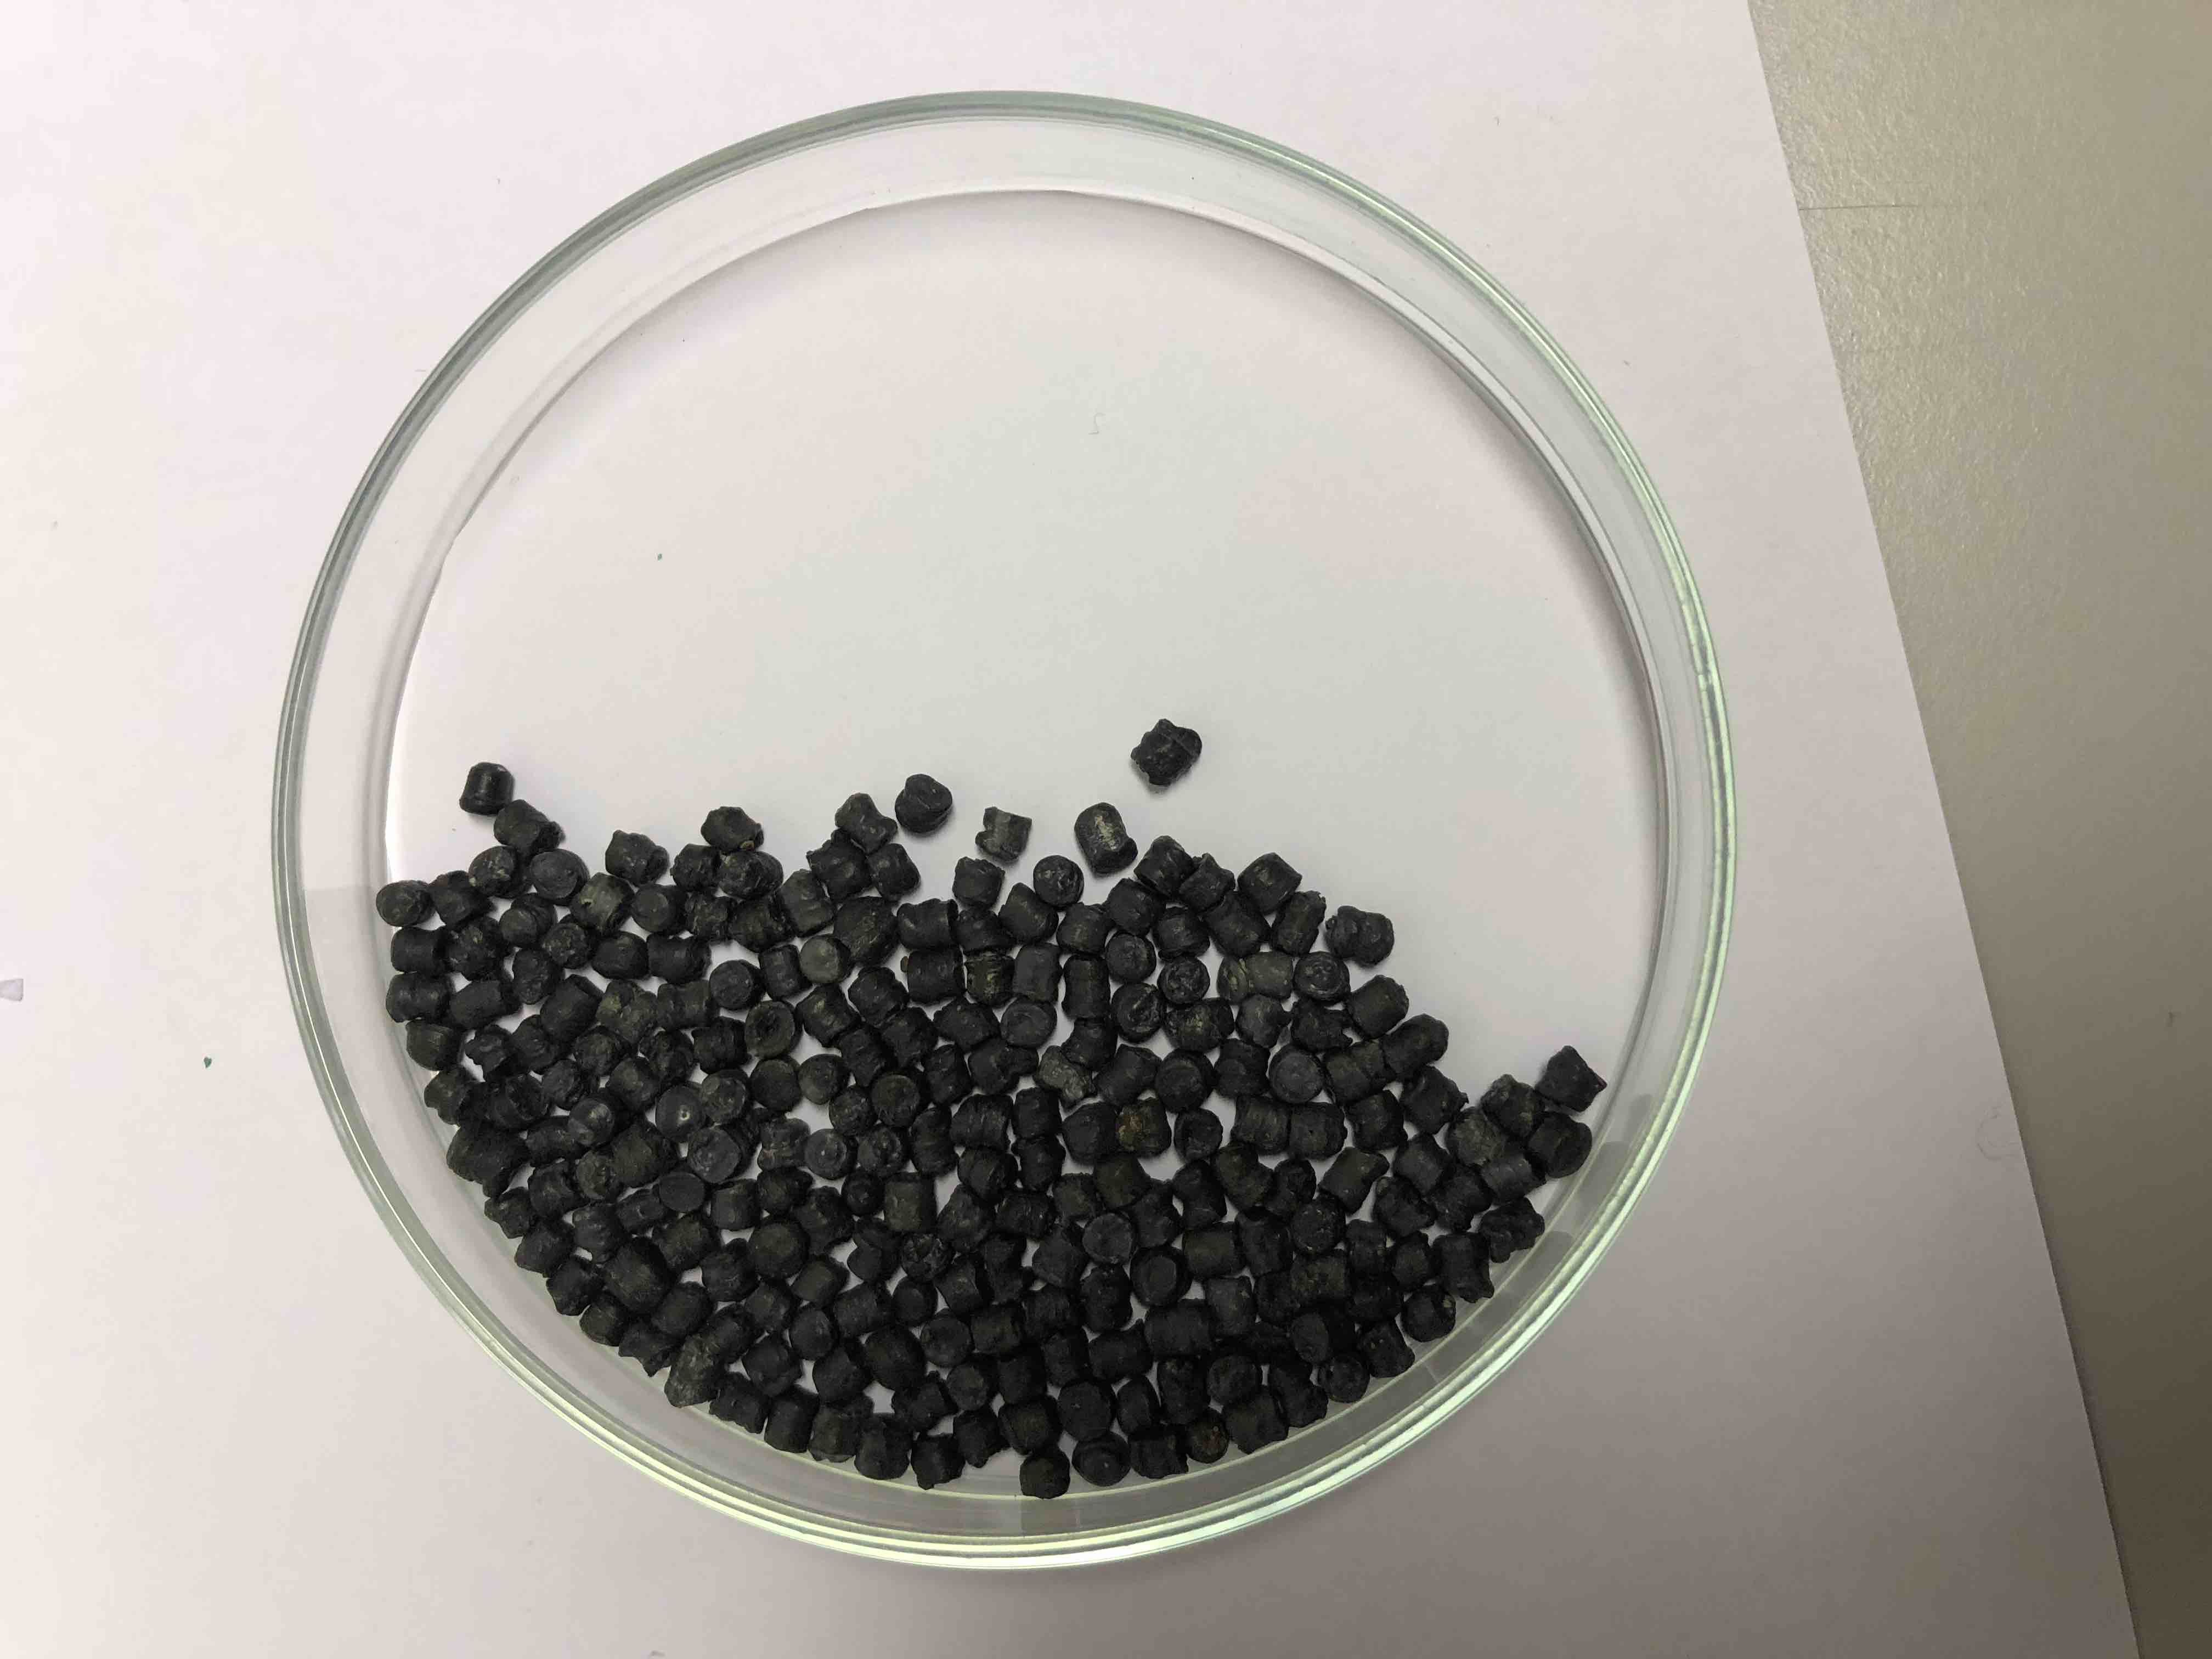
\includegraphics[width = 12cm]{Images/appendix/PE-pellets-beached-texel-black.jpg}
    \caption{PE beach-pellets, black}
    \label{fig:pe_beach_b}
\end{figure}

\begin{figure}
    \centering
    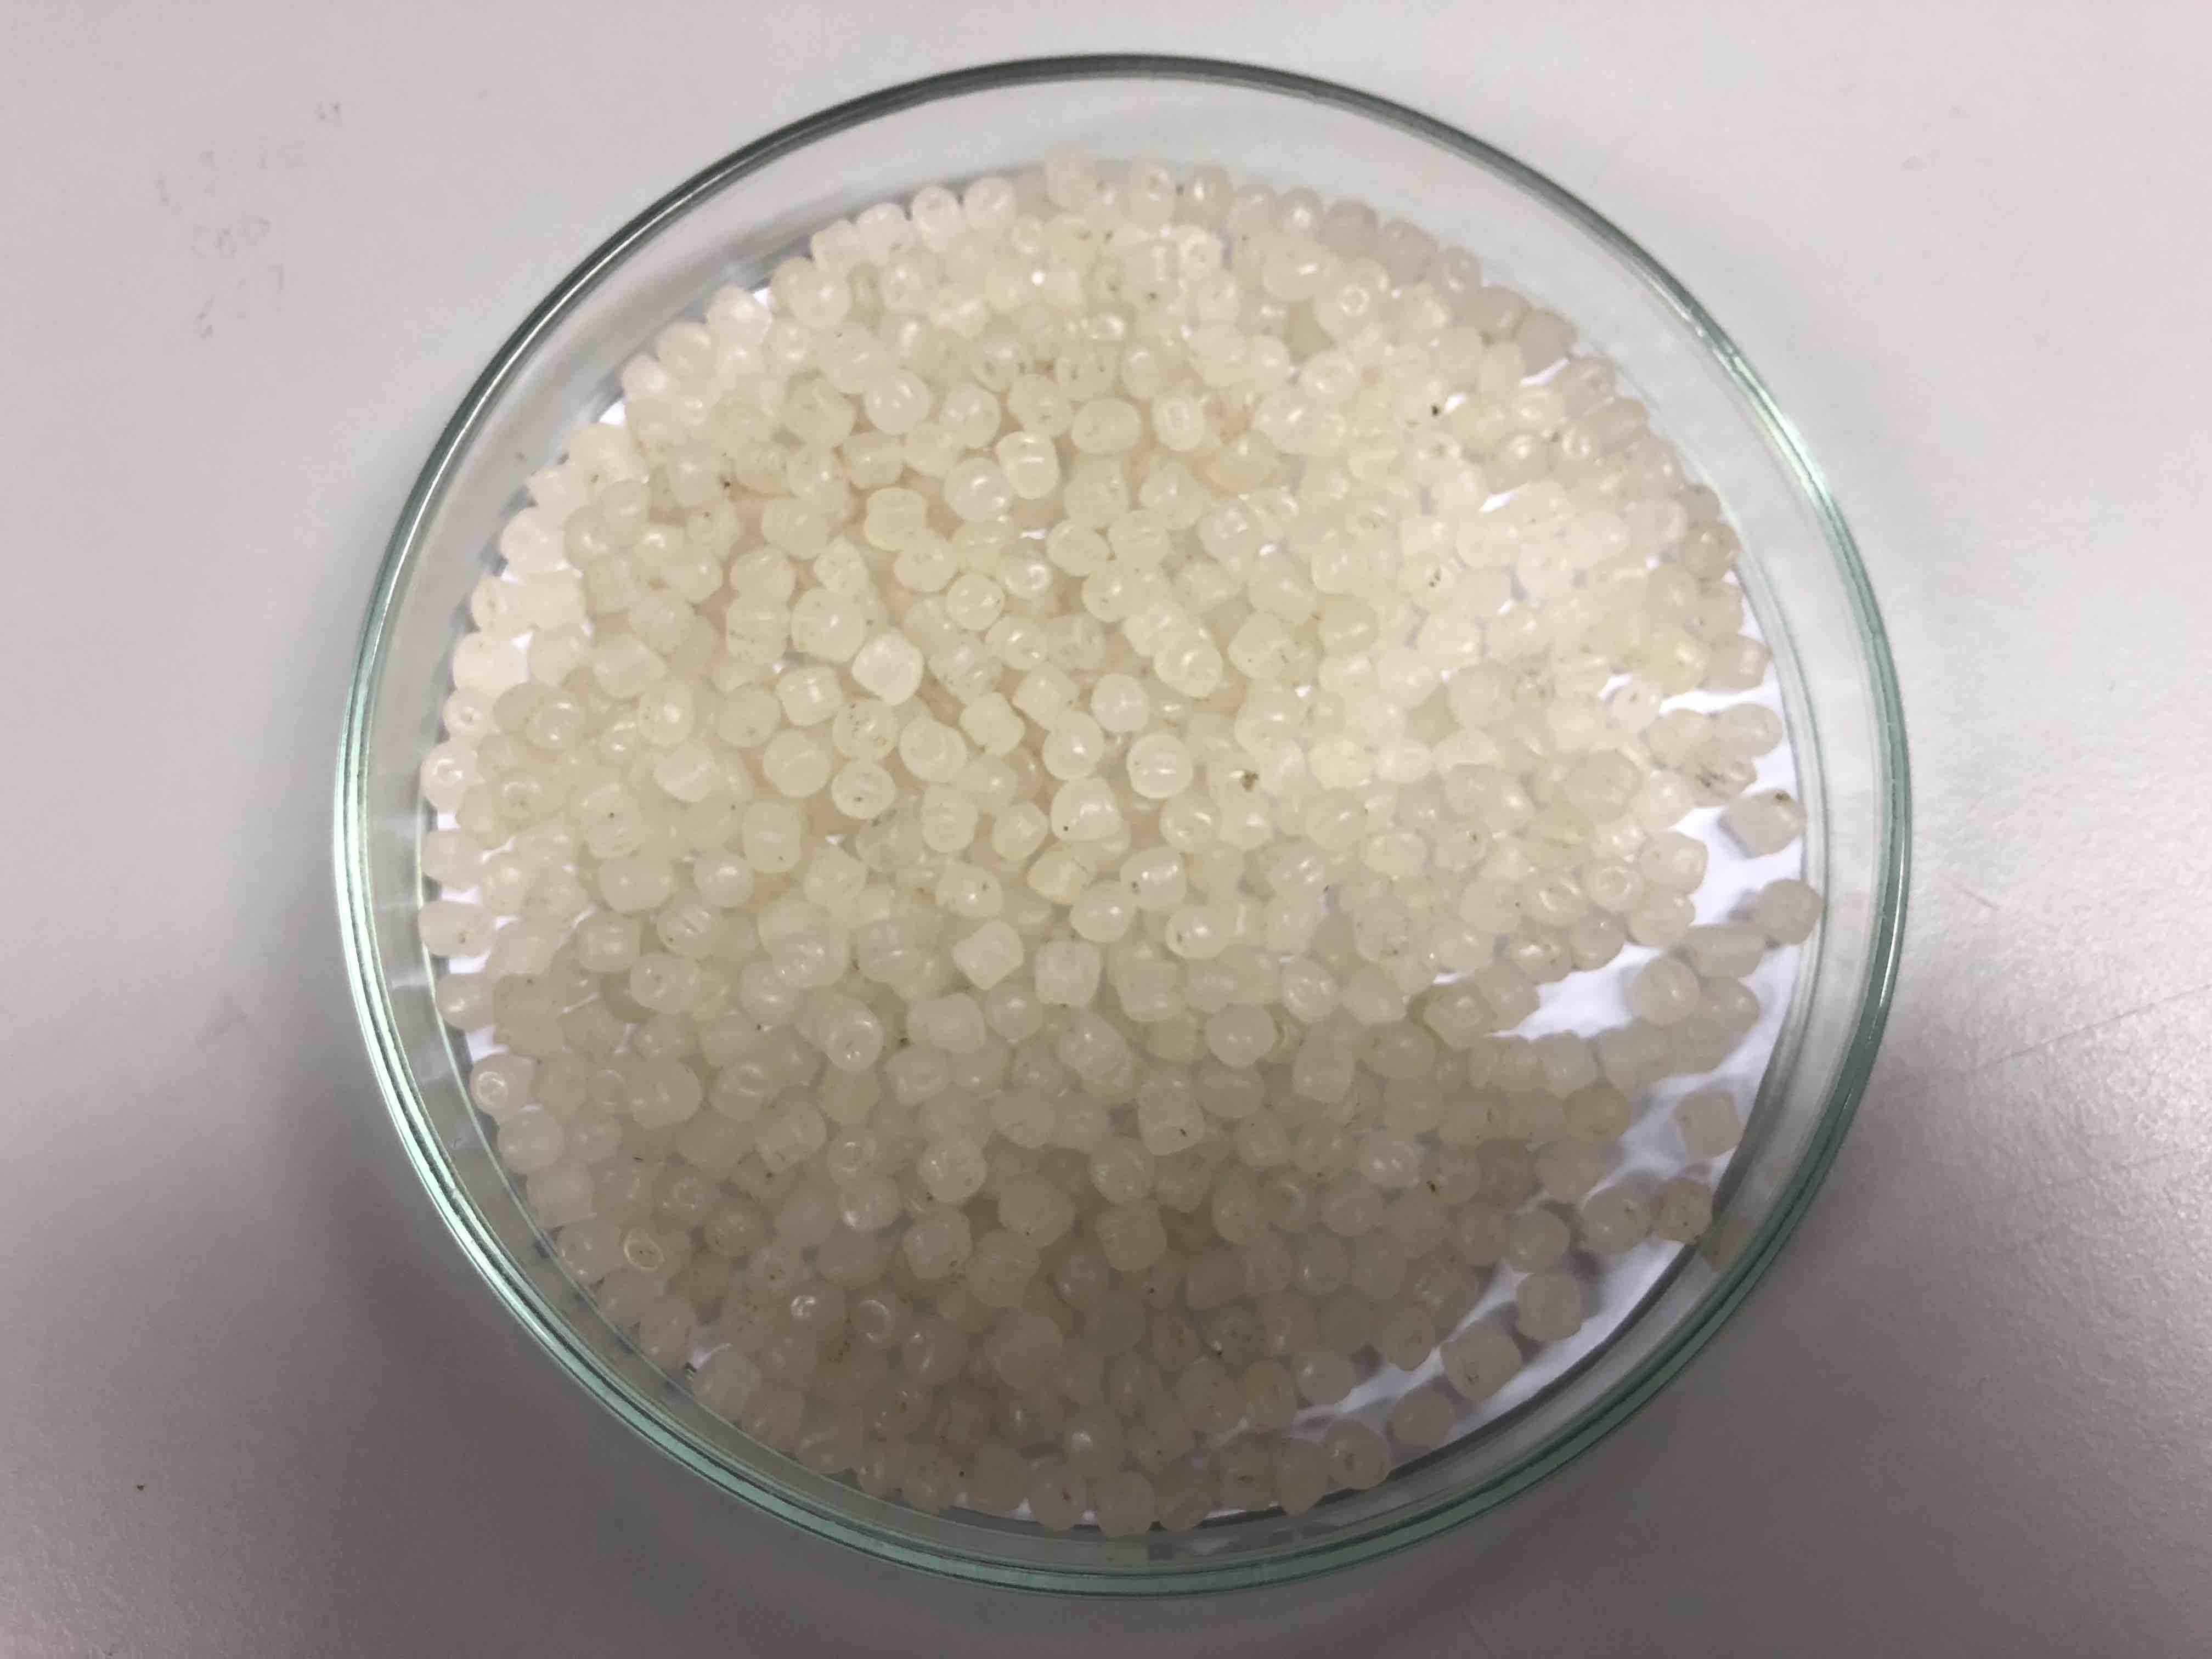
\includegraphics[width = 12cm]{Images/appendix/PE-pellets-beached-texel-white.jpg}
    \caption{PE beach-pellets, white}
    \label{fig:pe_beach_w}
\end{figure}

\begin{figure}
    \centering
    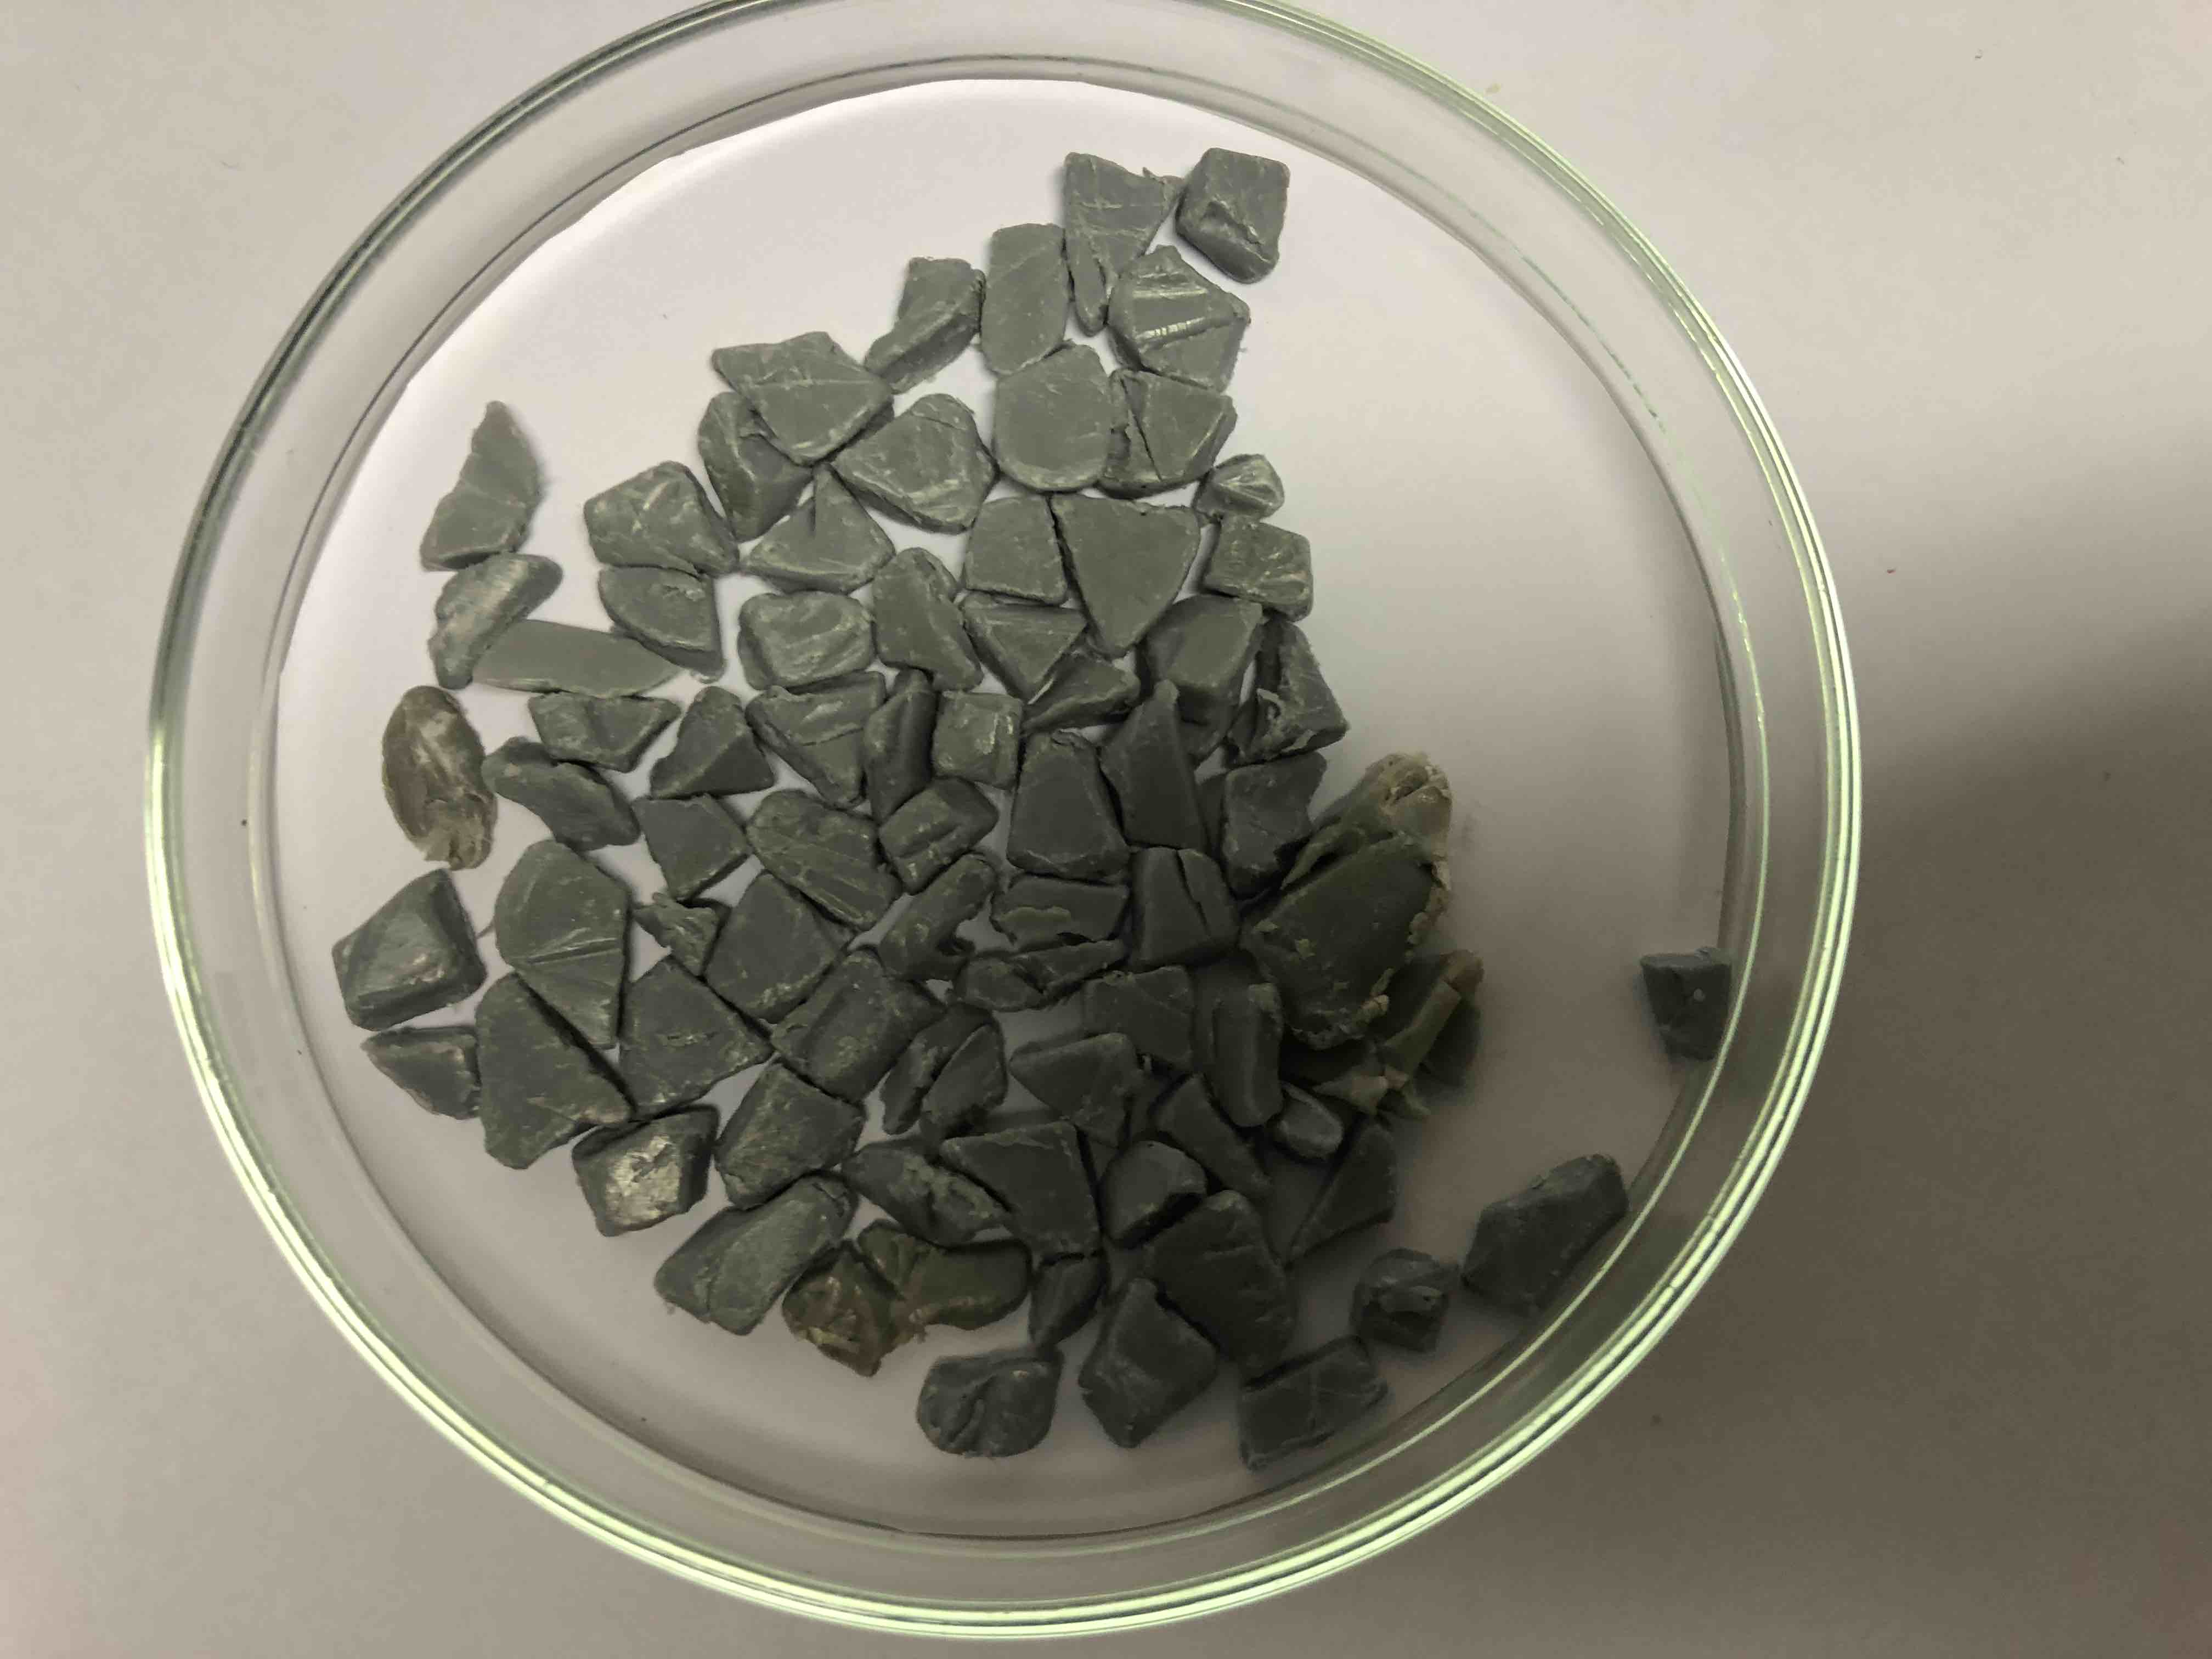
\includegraphics[width = 12cm]{Images/appendix/PE-Regrind-(Post-Consumer)-gray.jpg}
    \caption{PE-HD Post Consumer, Gray}
    \label{fig:pehd-gray}
\end{figure}

\begin{figure}
    \centering
    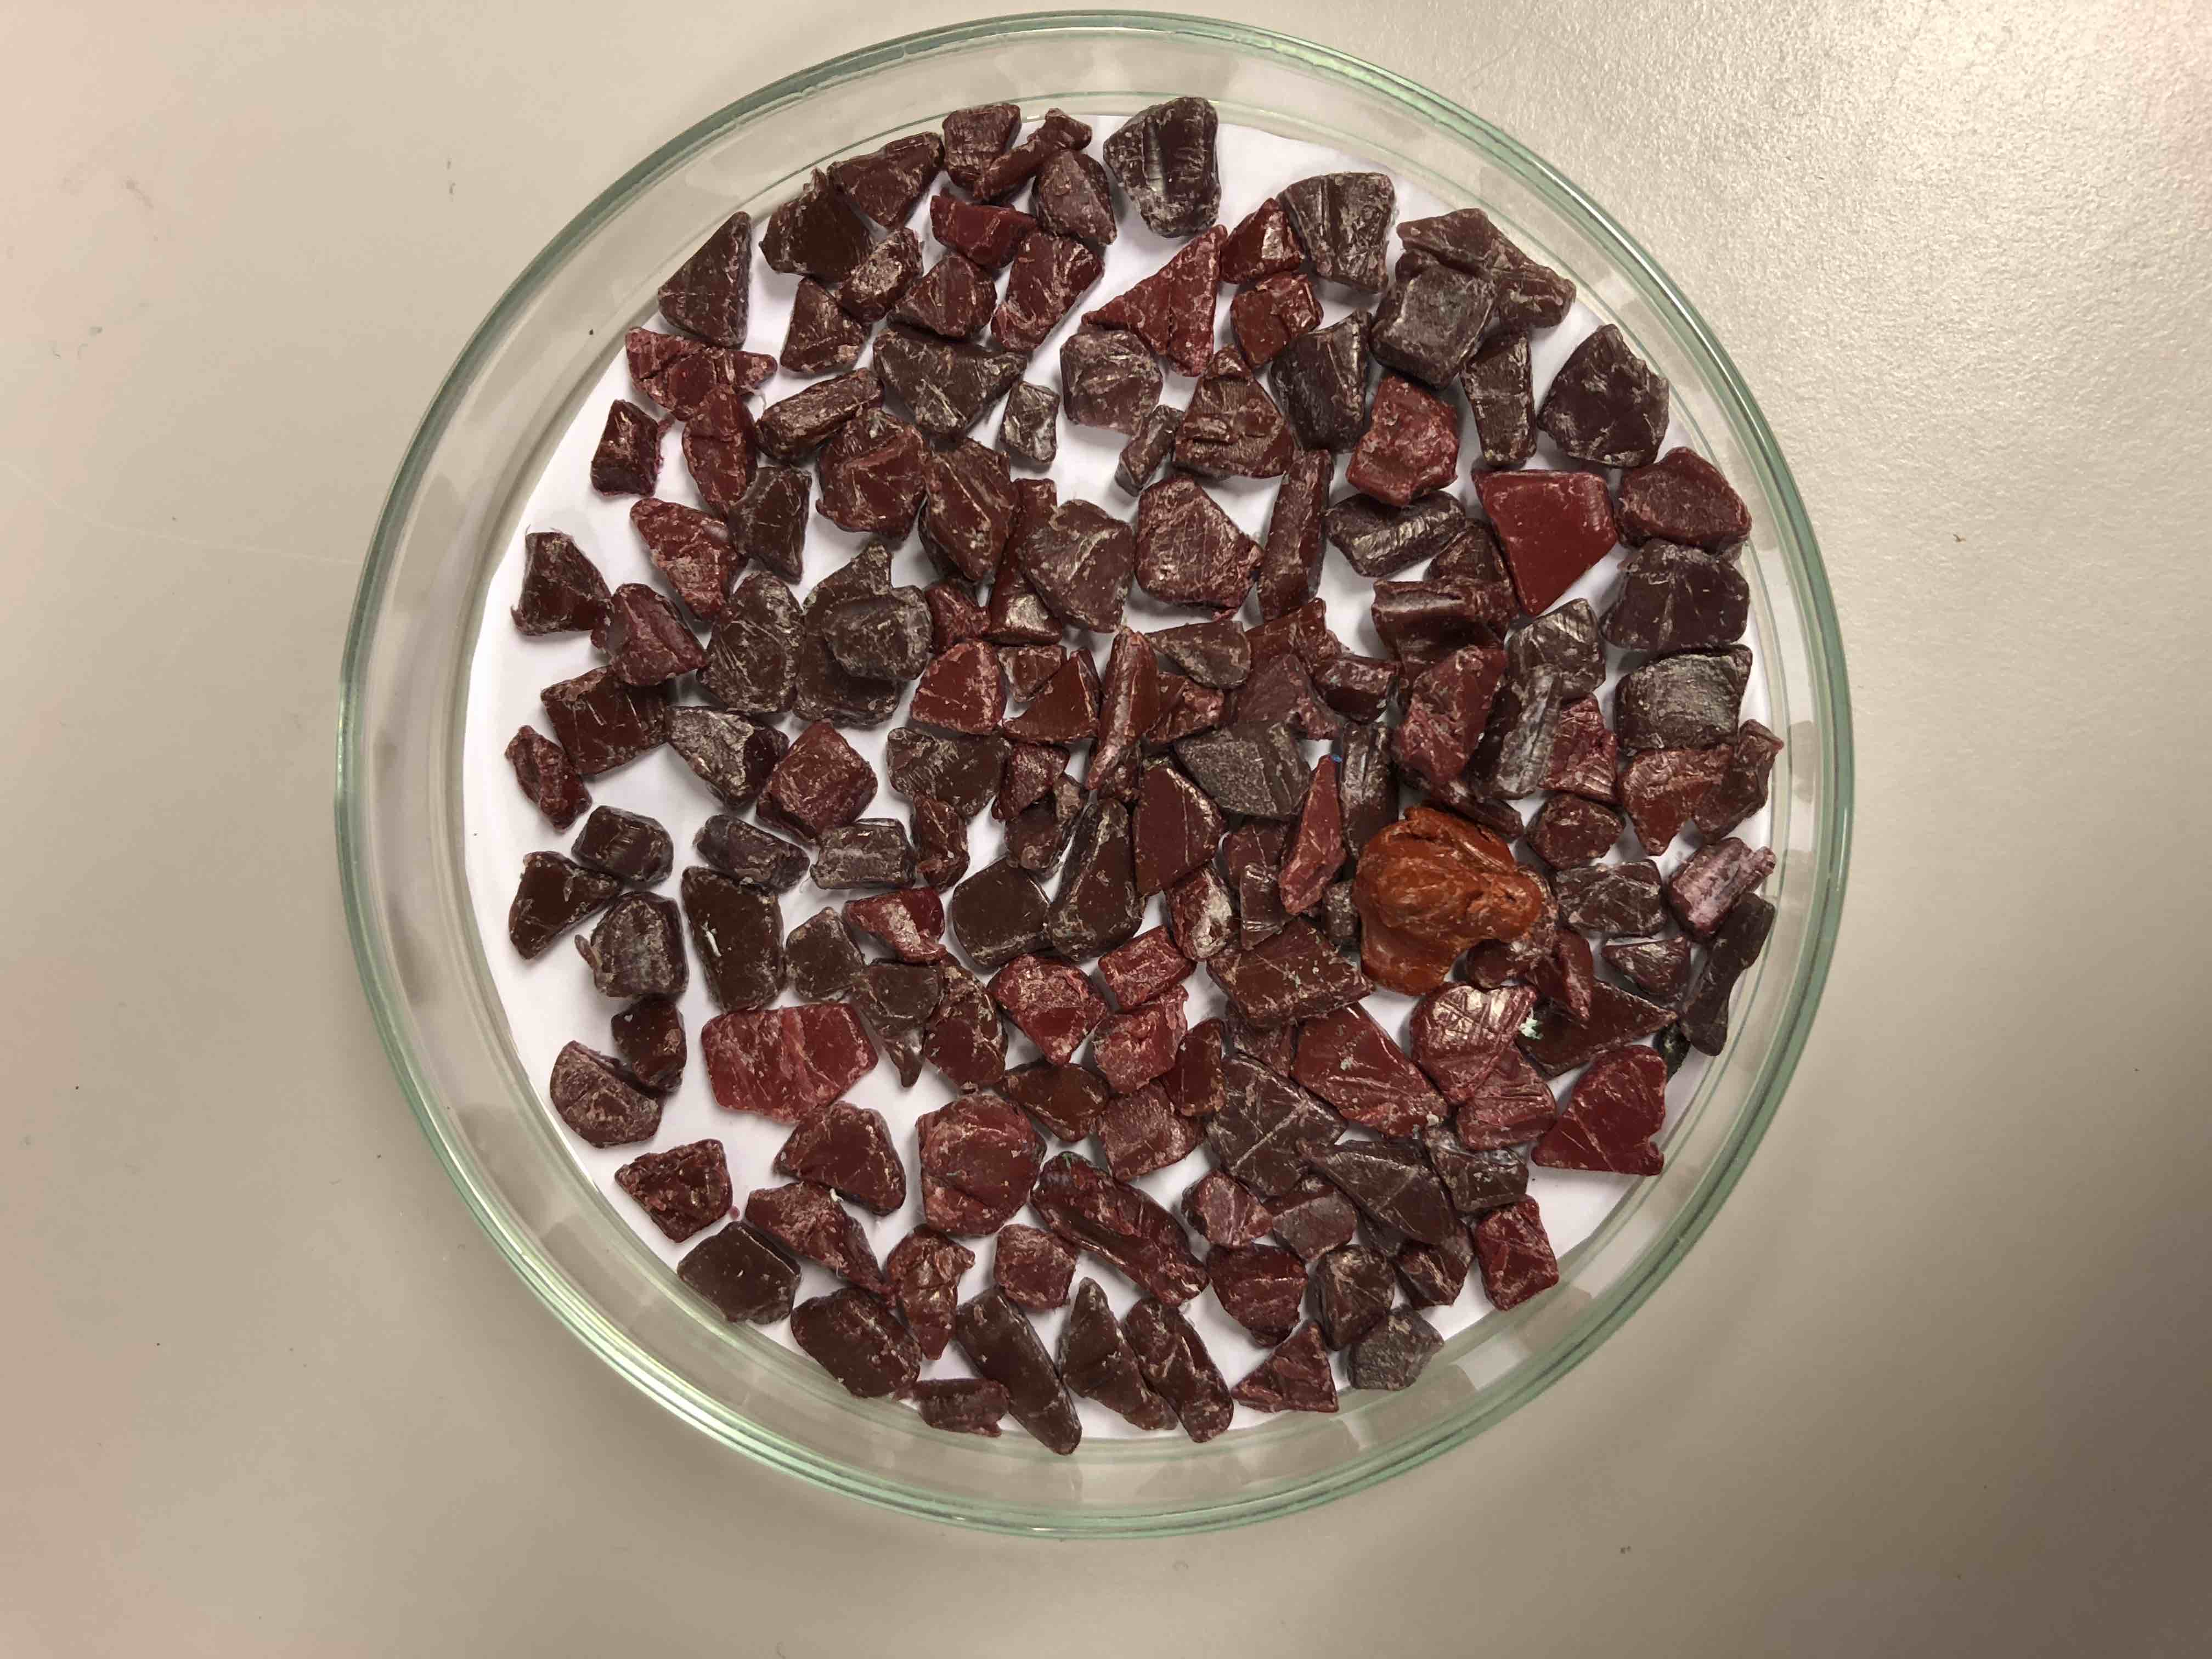
\includegraphics[width = 12cm]{Images/appendix/PE-Regrind-(Post-Consumer)-red.jpg}
    \caption{PE-HD Post Consumer, Red}
    \label{fig:pehd-red}
\end{figure}

\begin{figure}
    \centering
    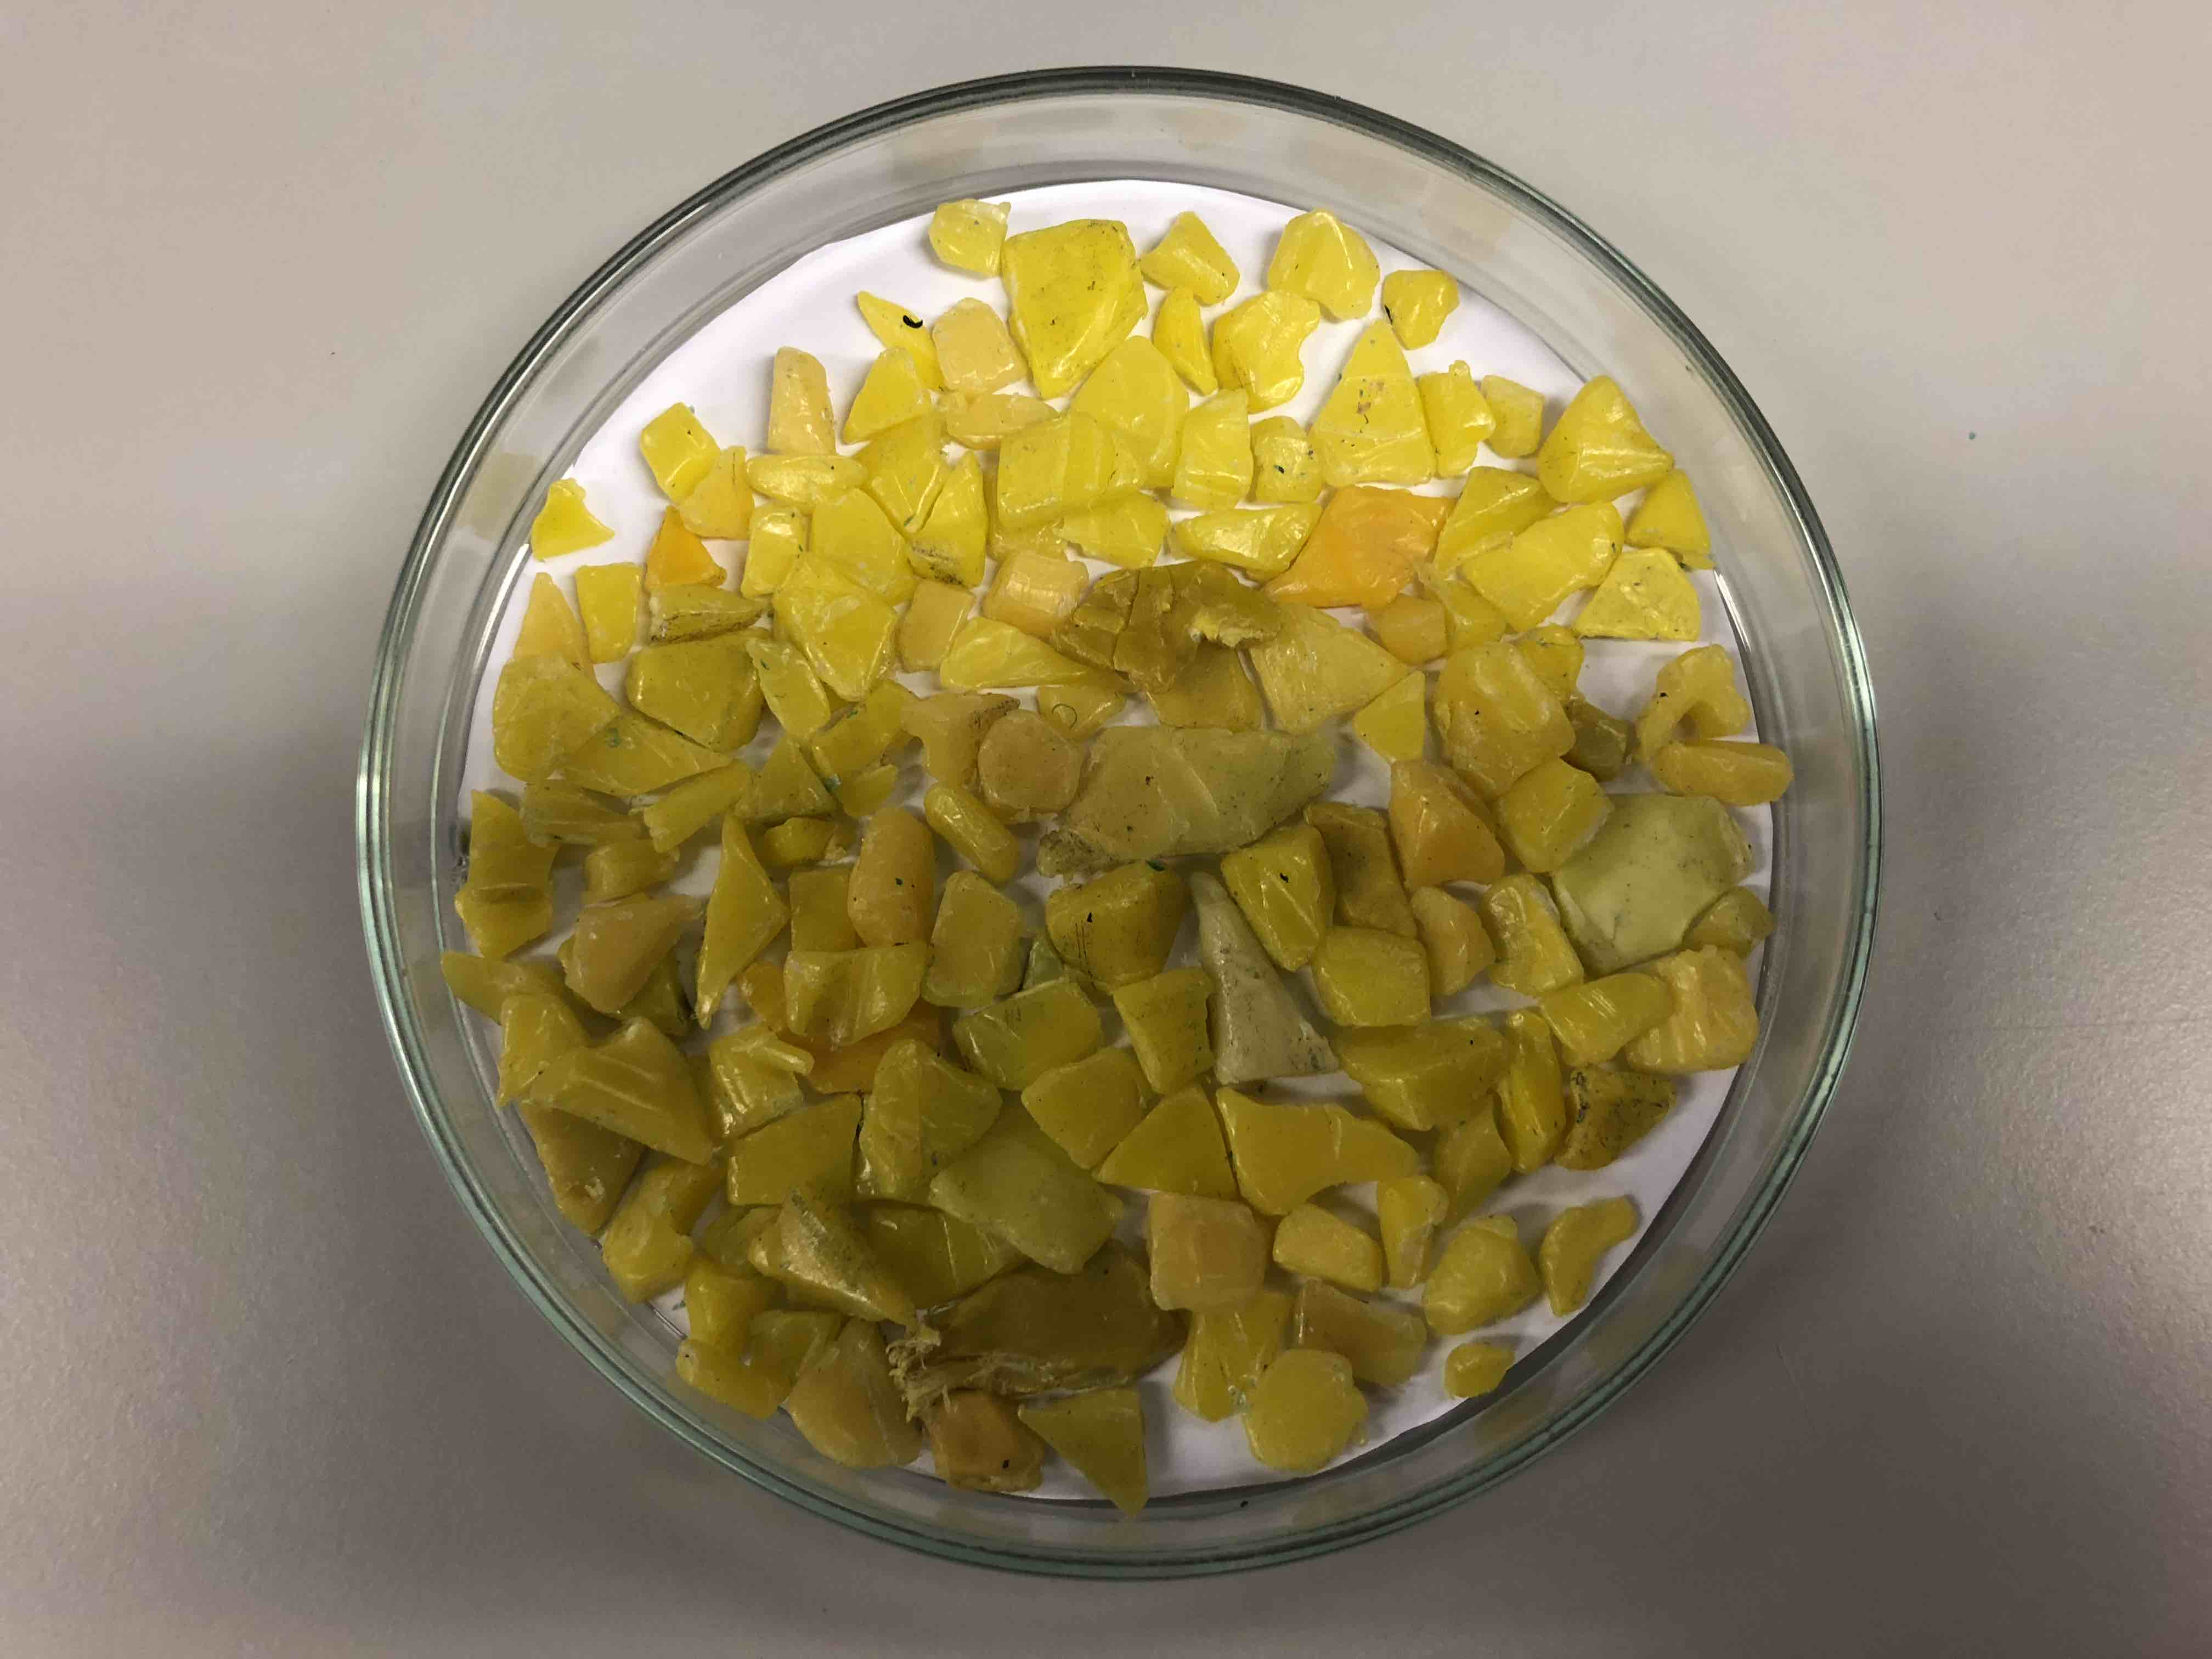
\includegraphics[width = 12cm]{Images/appendix/PE-Regrind-(Post-Consumer)-yellow.jpg}
    \caption{PE-HD Post Consumer, Yellow}
    \label{fig:pehd-yellow}
\end{figure}

\begin{figure}
    \centering
    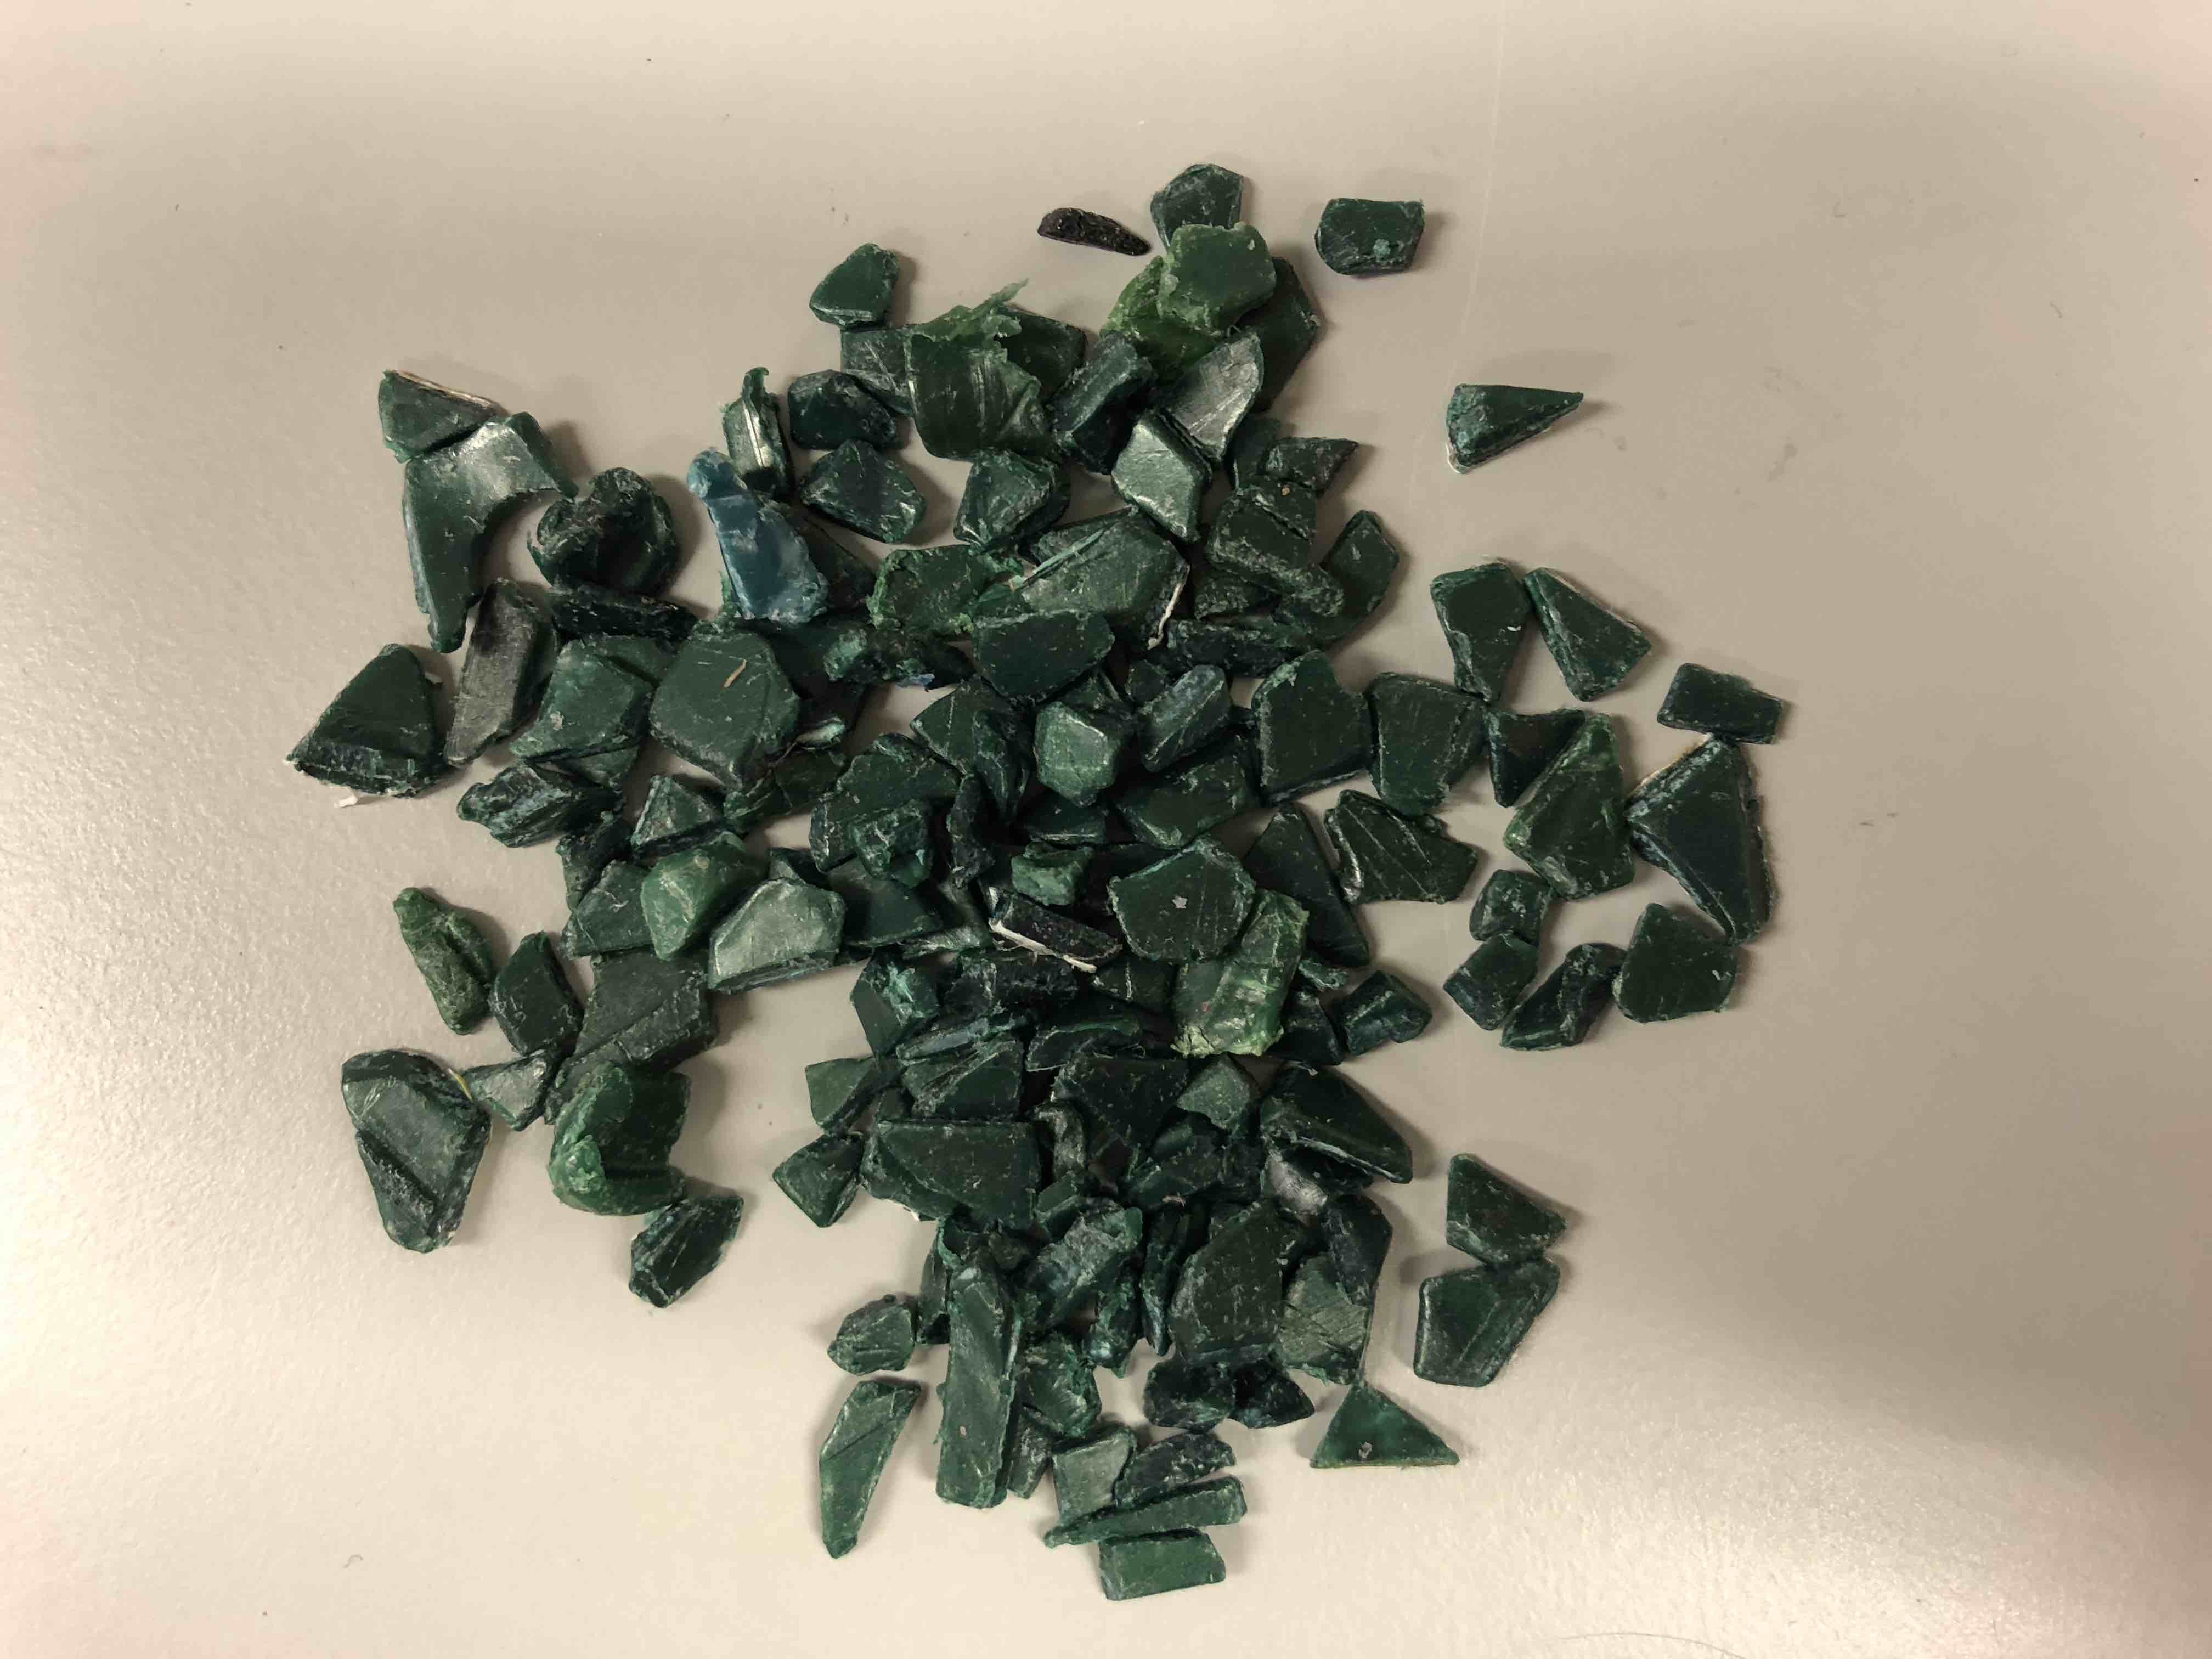
\includegraphics[width = 12cm]{Images/appendix/PE-Regrind-(Post-Consumer)-green.jpg}
    \caption[$\; \:$PE-HD Post Consumer, Green]{PE-HD, Post Consumer, Green}
    \label{fig:pehd-green}
\end{figure}

\begin{figure}
    \centering
    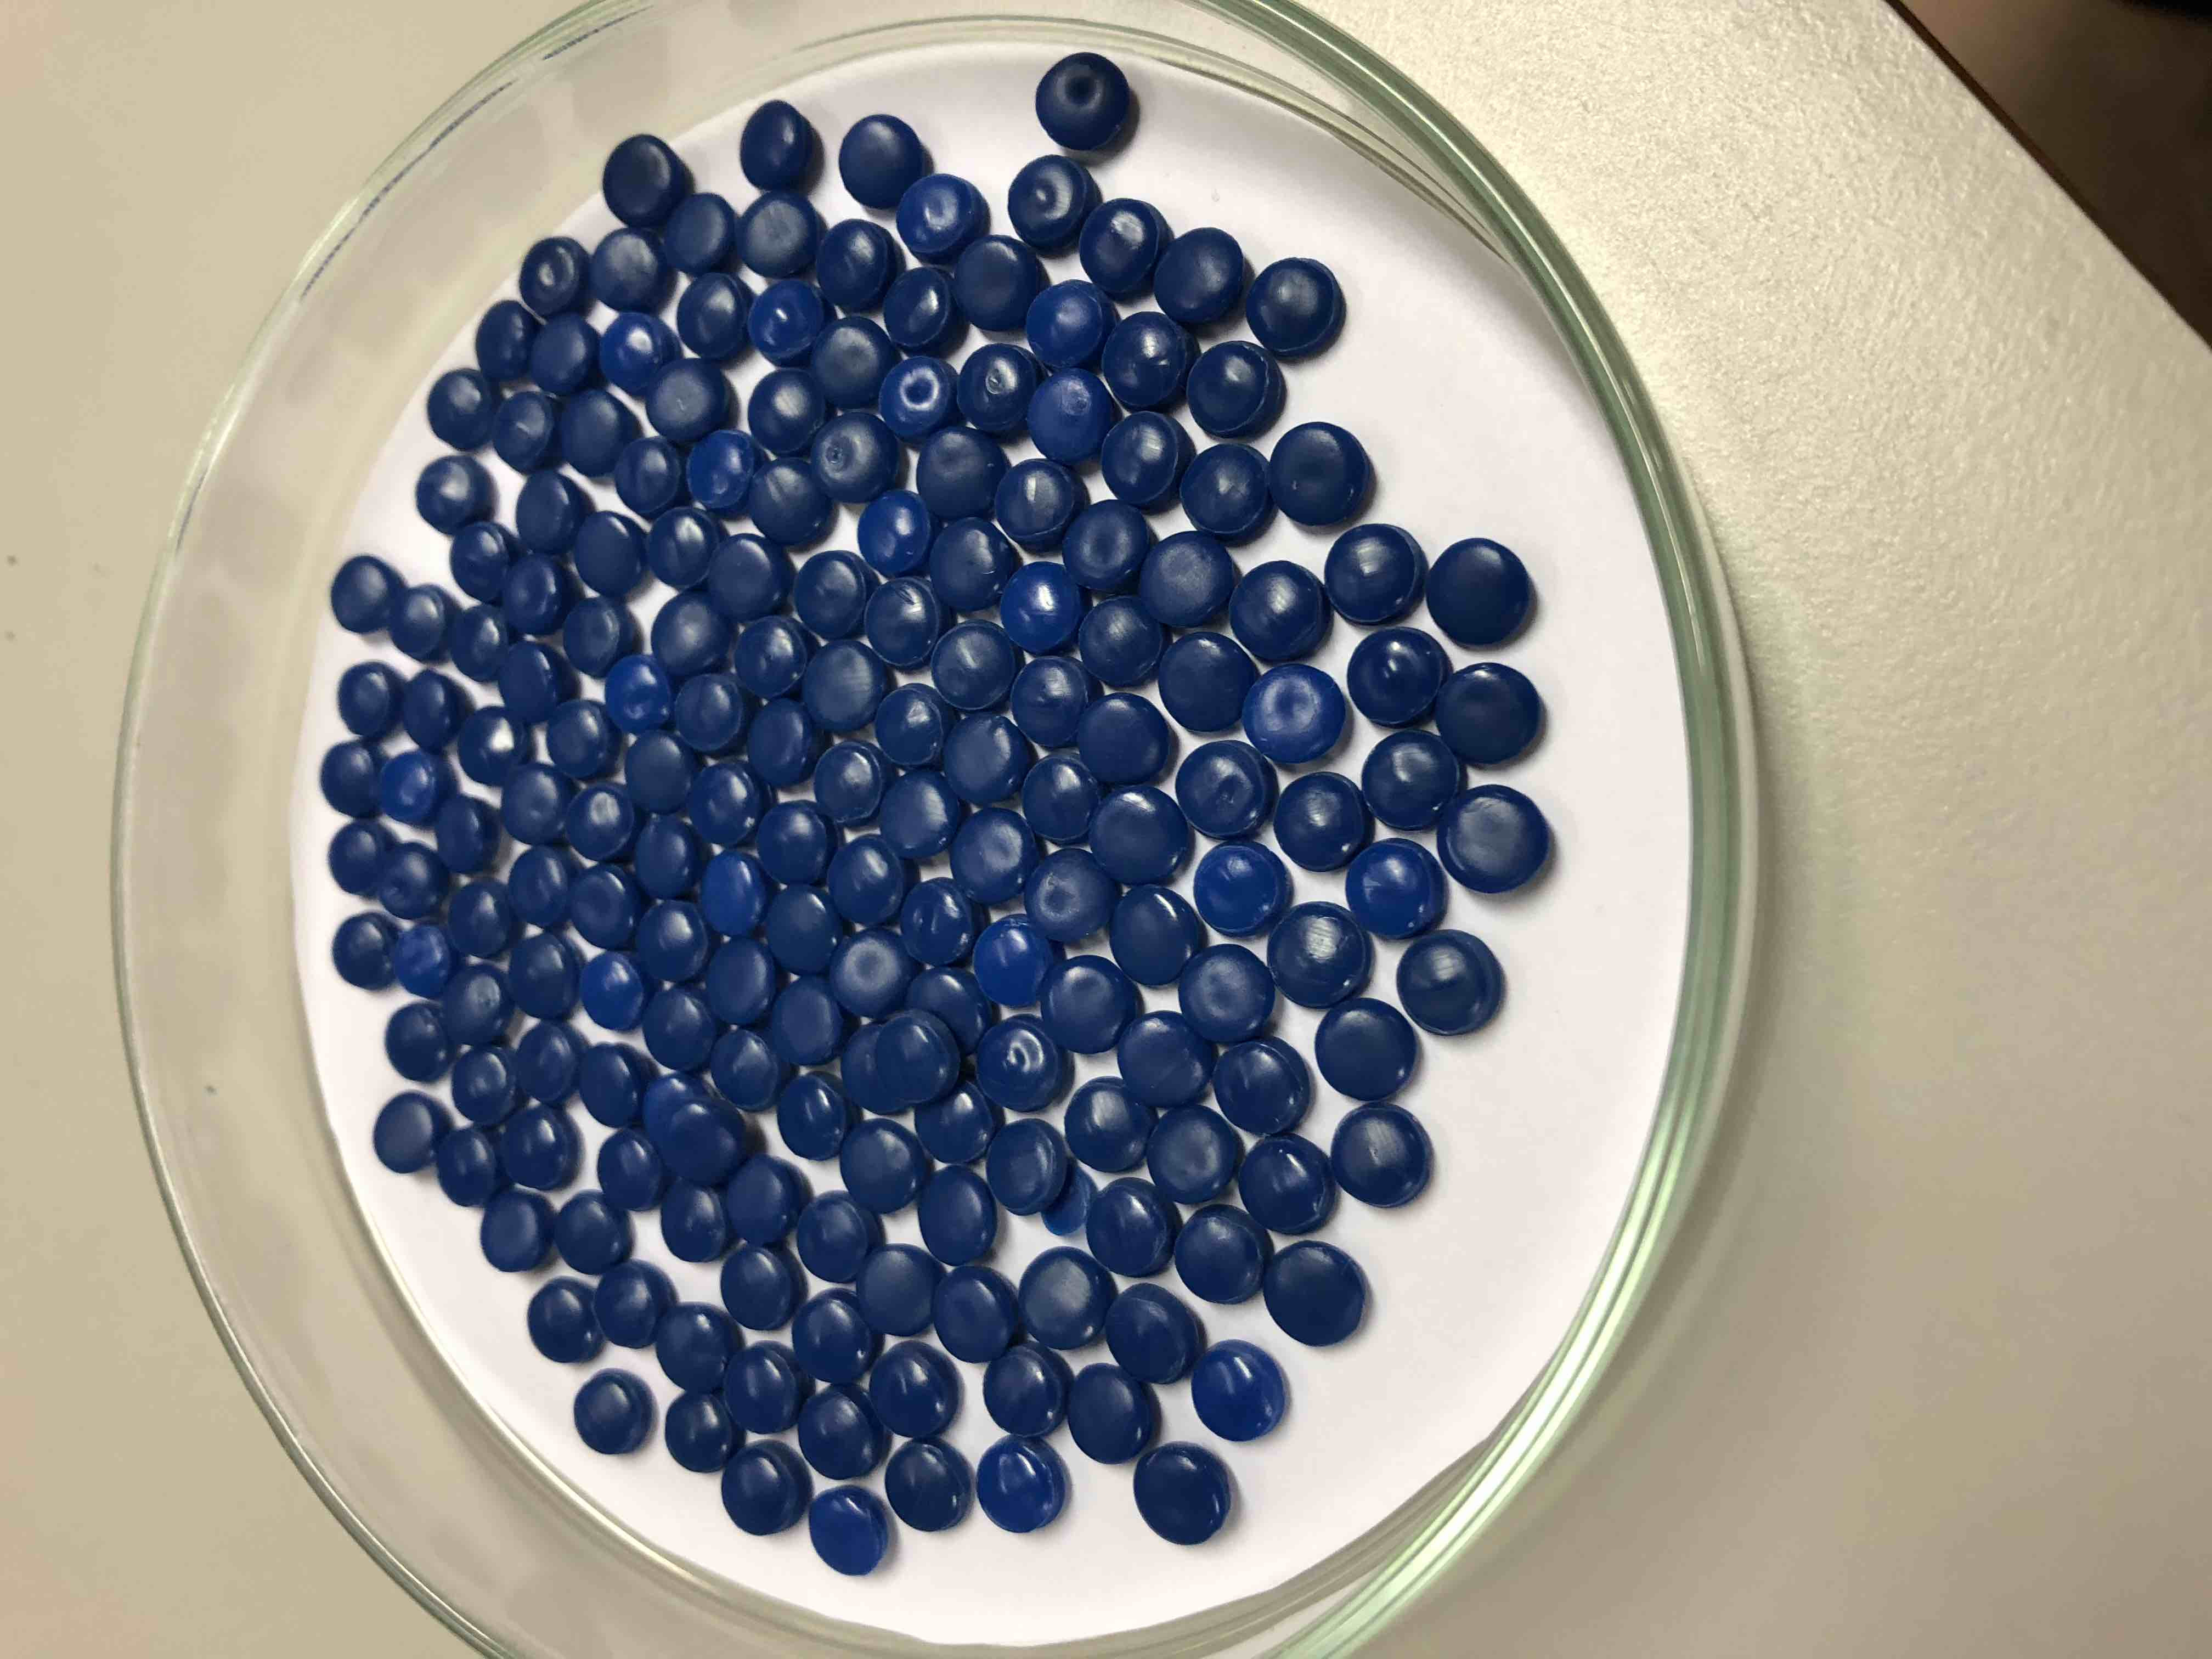
\includegraphics[width = 12cm]{Images/appendix/PE-Recyclate-(Post-Industrial)-blue.jpg}
    \caption[$\; \:$PE-LD Post Industrial, Blue]{PE-LD, Post Industrial, Blue}
    \label{fig:peld-blue}
\end{figure}

\begin{figure}
    \centering
    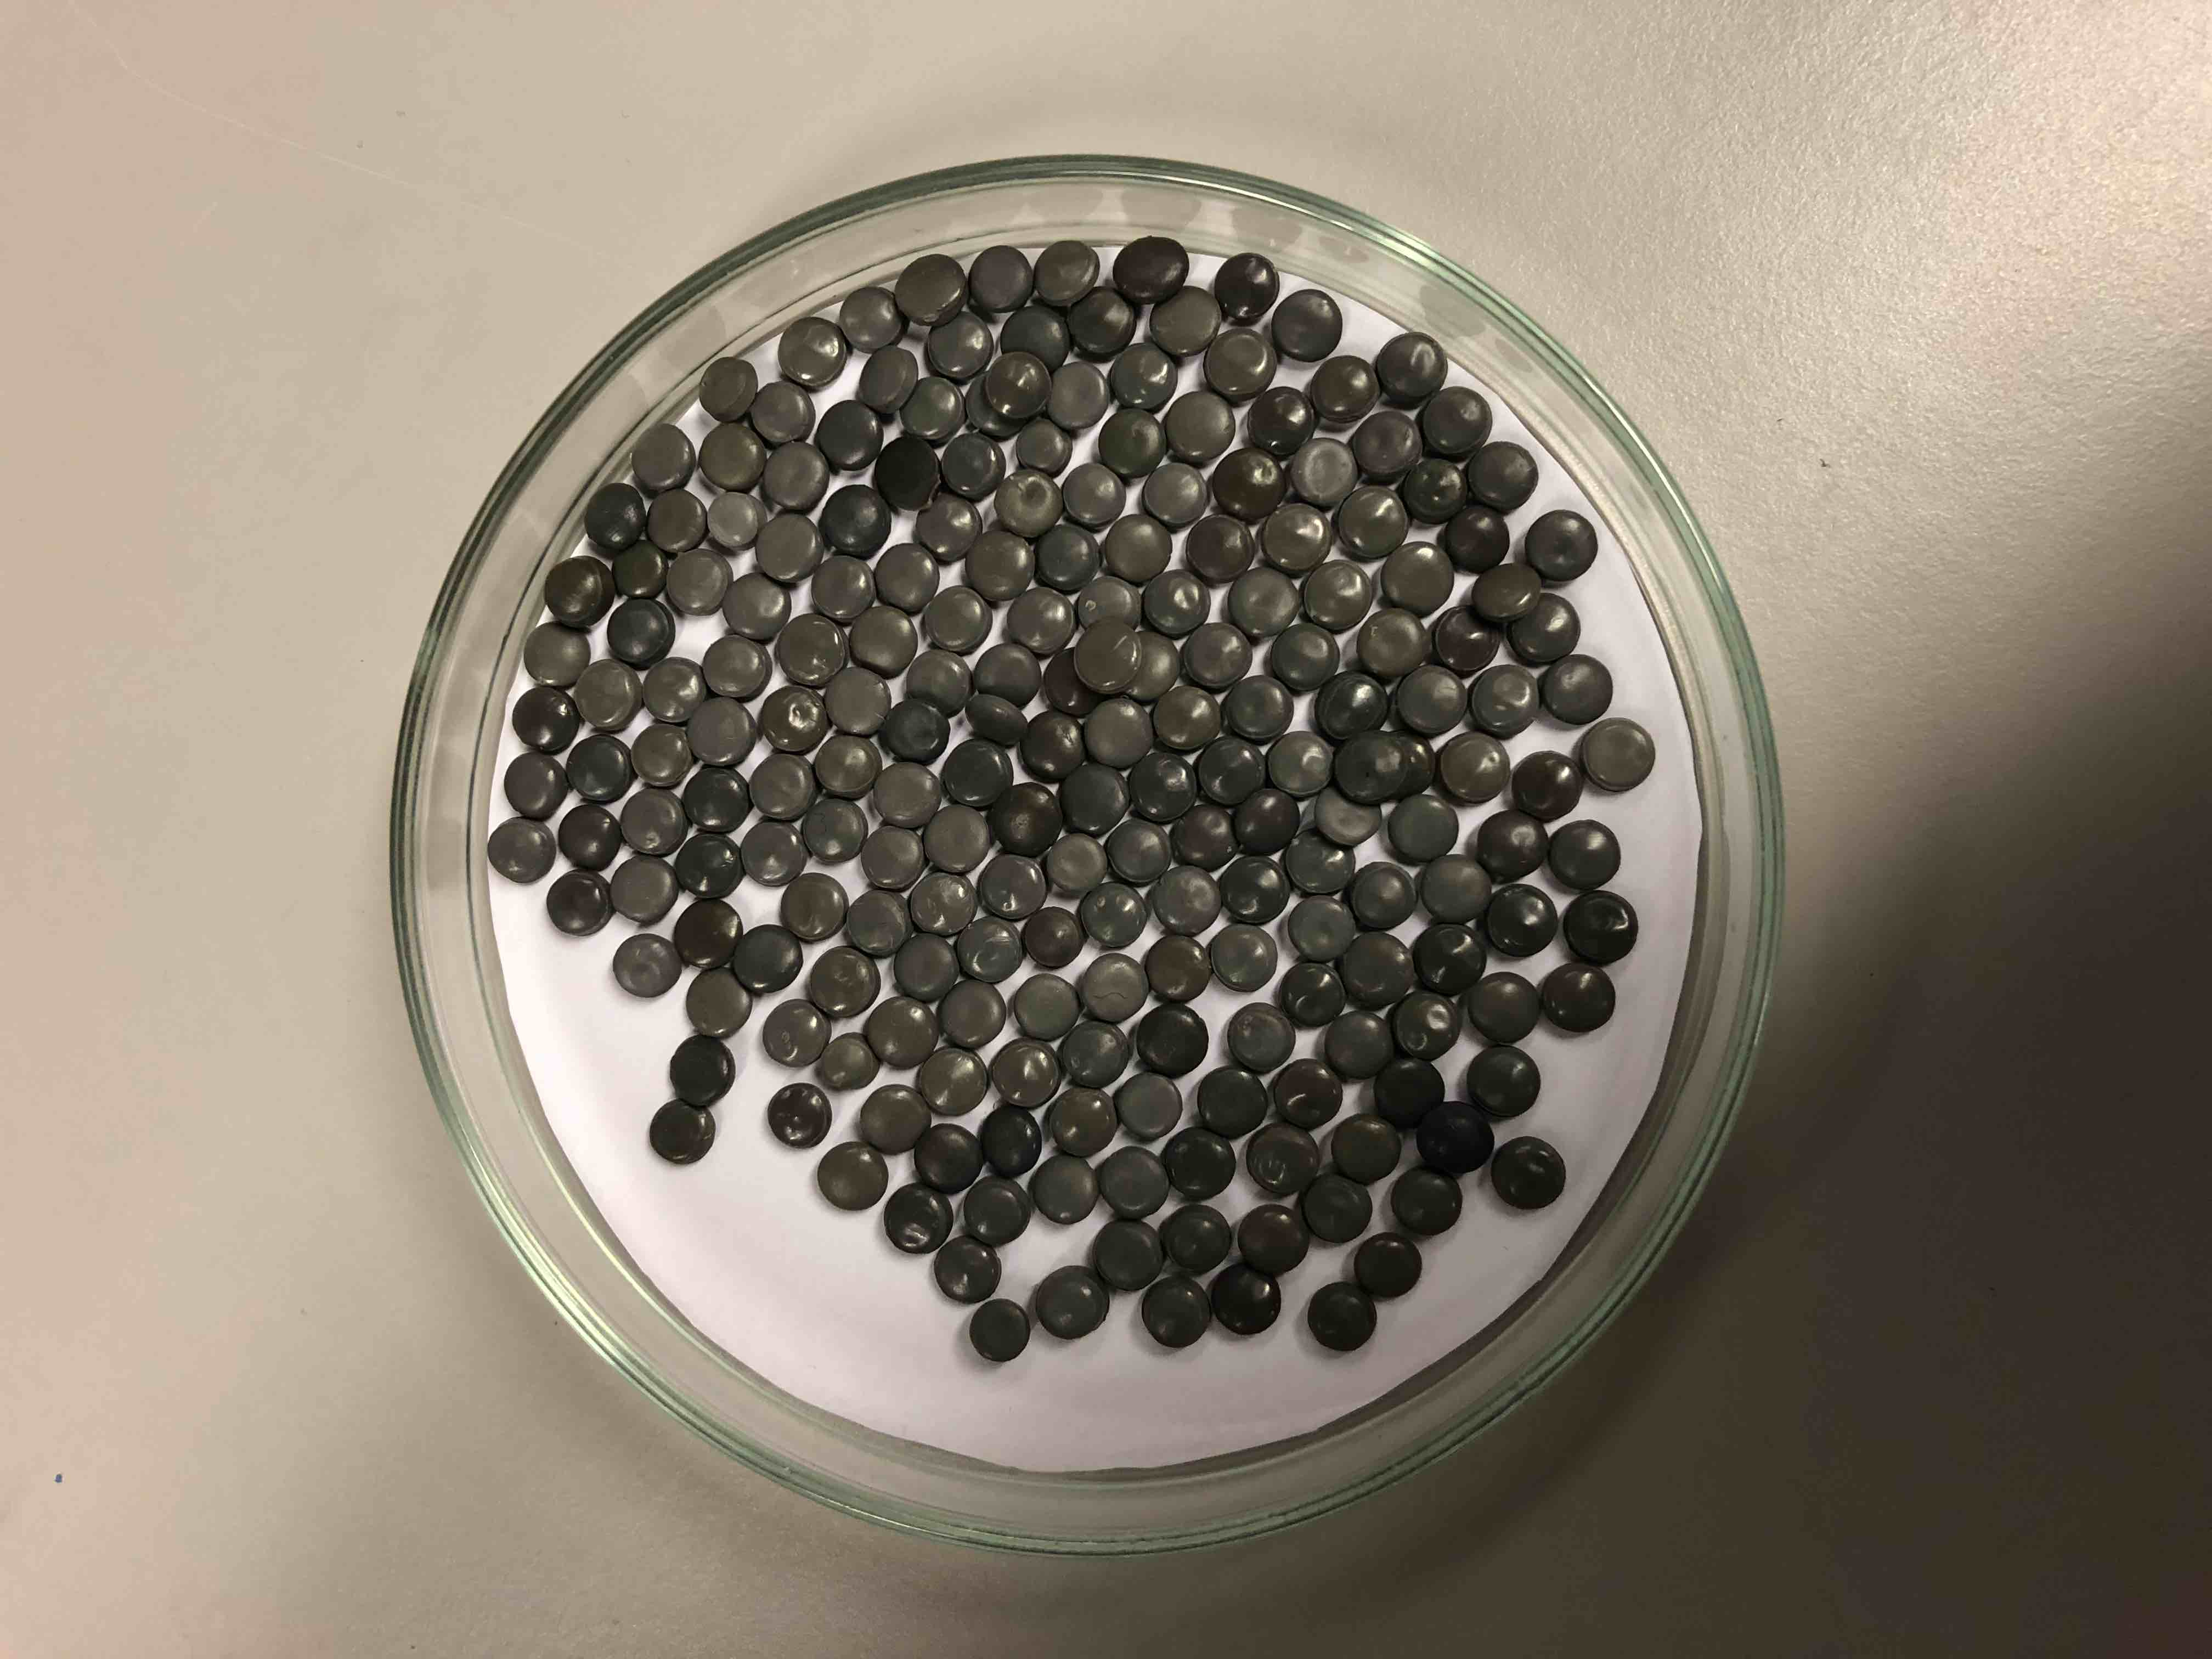
\includegraphics[width = 12cm]{Images/appendix/PE-Recyclate-(Post-Industrial)-gray.jpg}
    \caption[$\; \:$PE-LD Post Industrial, Gray]{PE-LD, Post Industrial, Gray}
    \label{fig:peld-gray}
\end{figure}

\begin{figure}
    \centering
    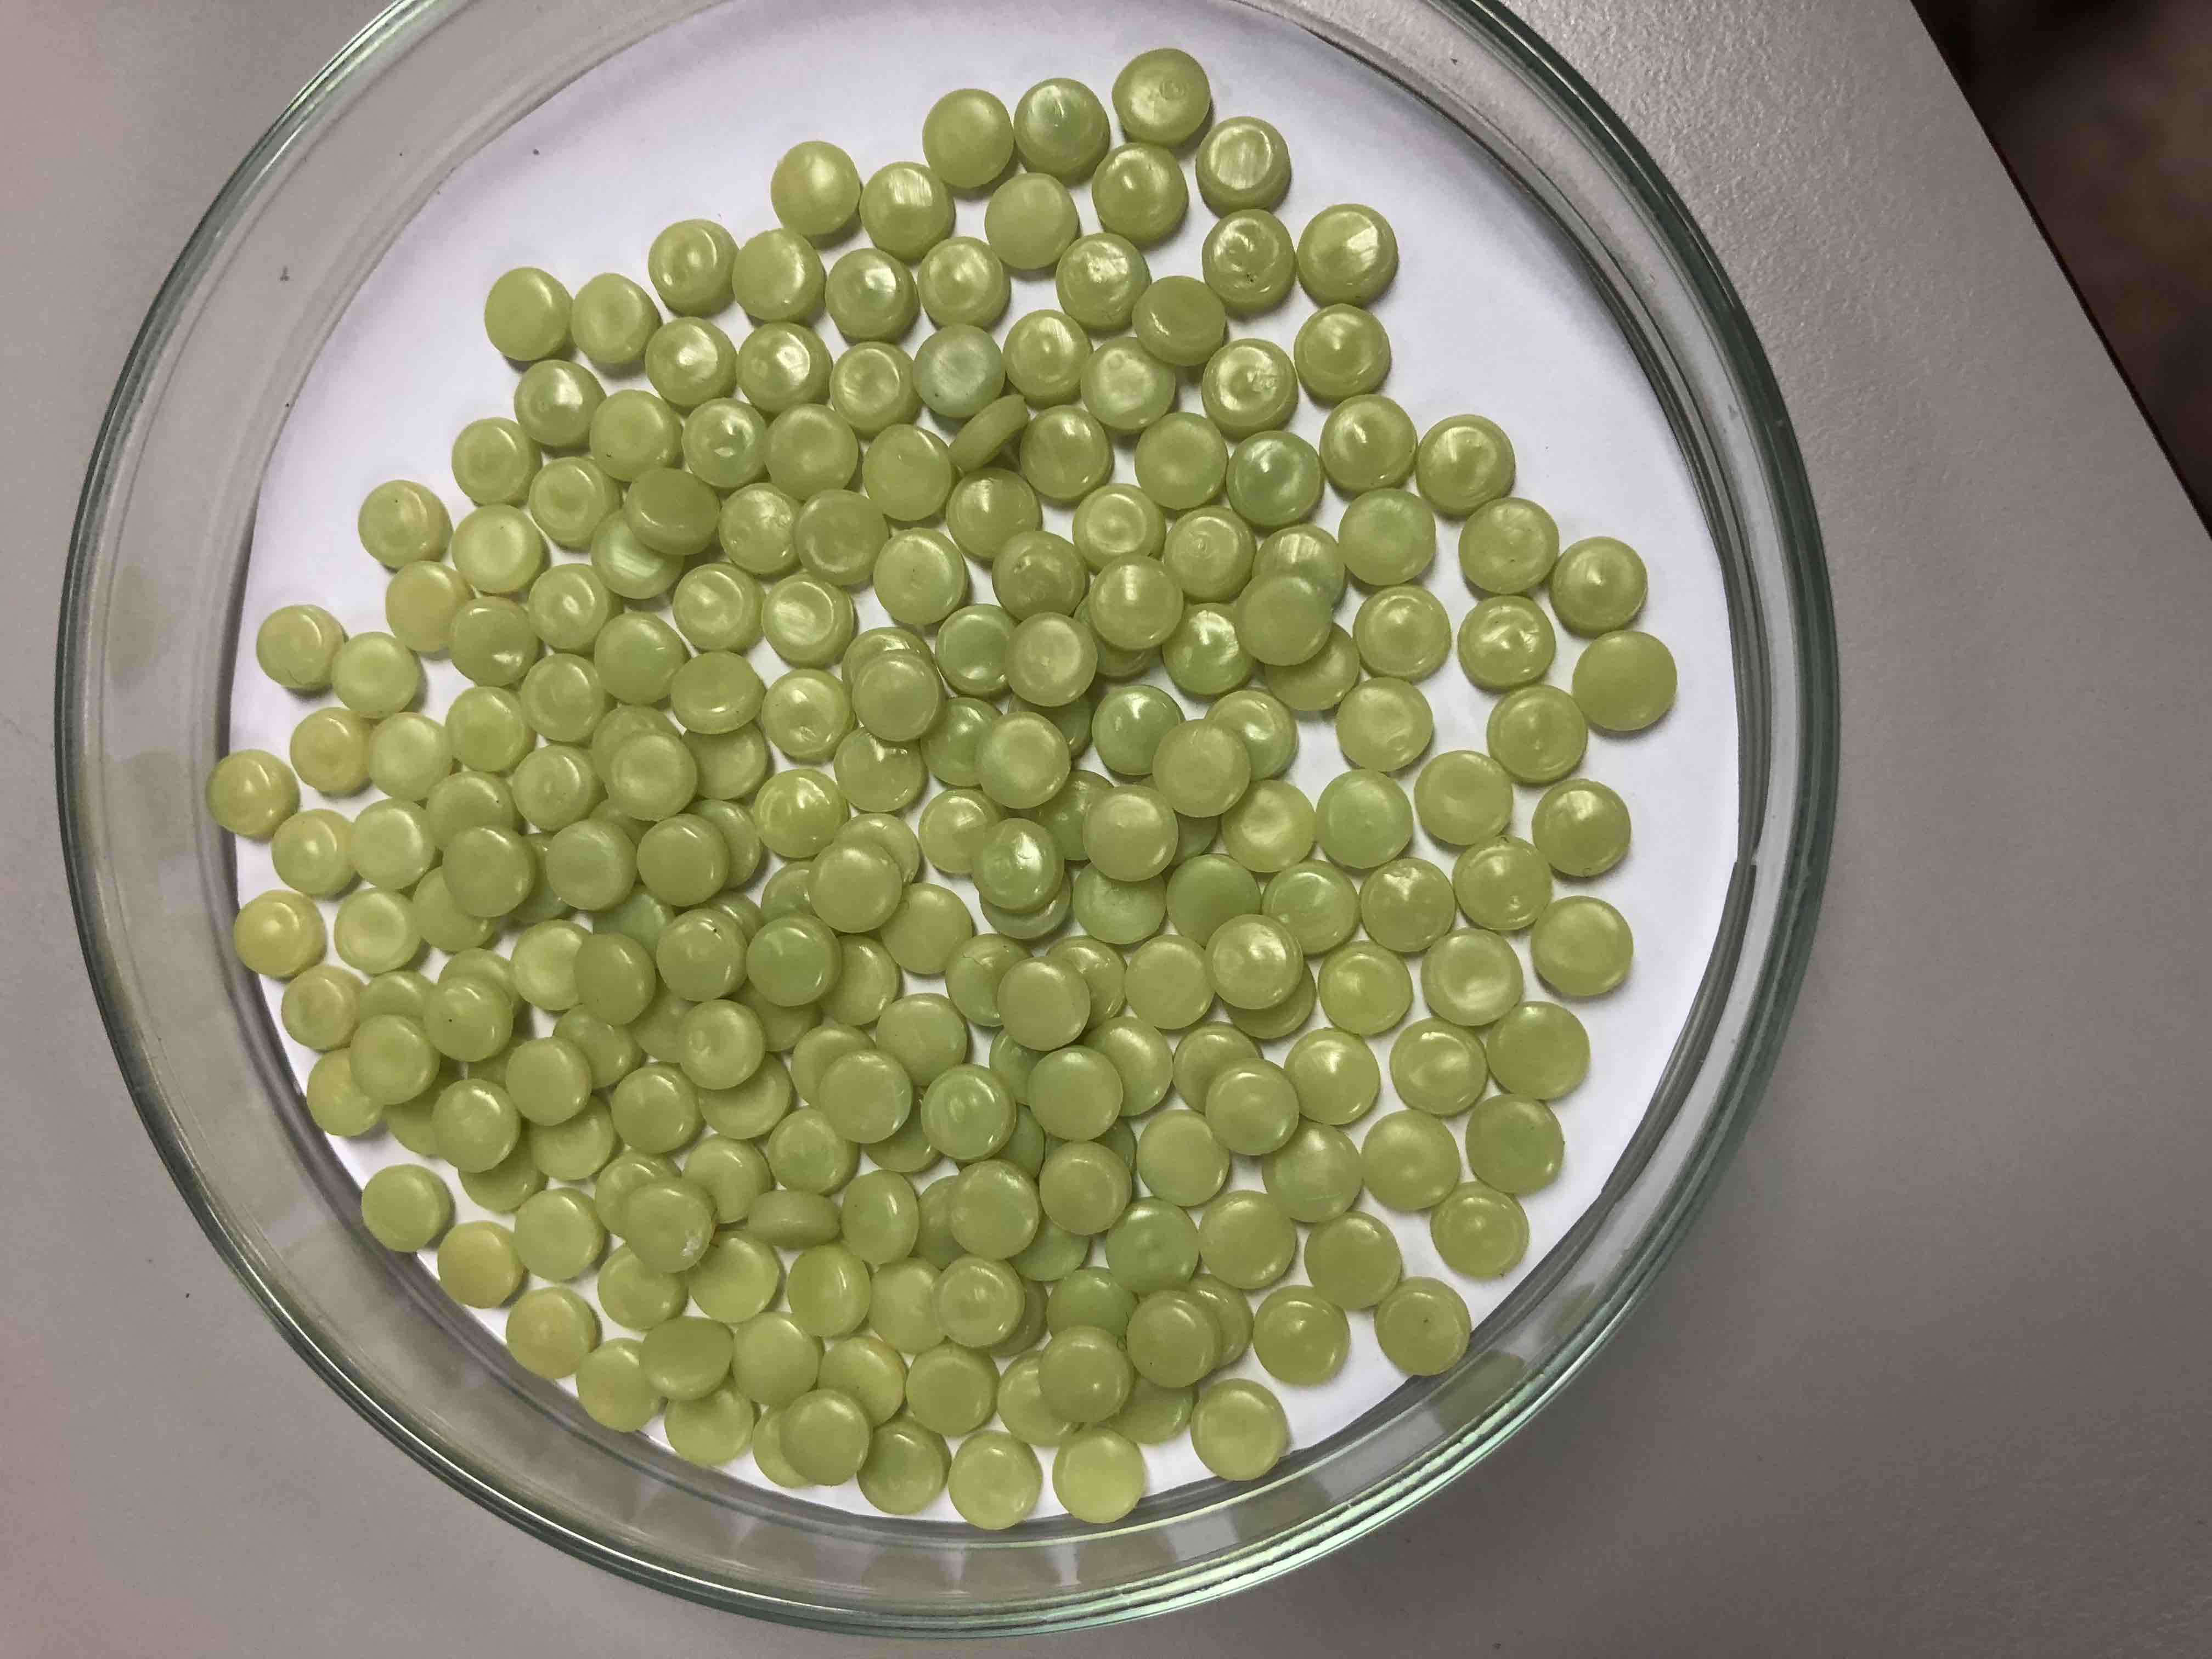
\includegraphics[width = 12cm]{Images/appendix/PE-Recyclate-(Post-Industrial)-lightgreen.jpg}
    \caption[$\; \:$PE-LD Post Industrial, Green]{PE-LD Post Industrial, Green}
    \label{fig:peld-green}
\end{figure}

\begin{figure}
    \centering
    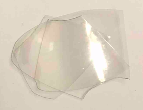
\includegraphics[width = 8cm]{Images/appendix/pepsi.png}
    \caption[$\; \:$Pepsi]{Pepsi}
    \label{fig:pepsi}
\end{figure}

\begin{figure}
    \centering
    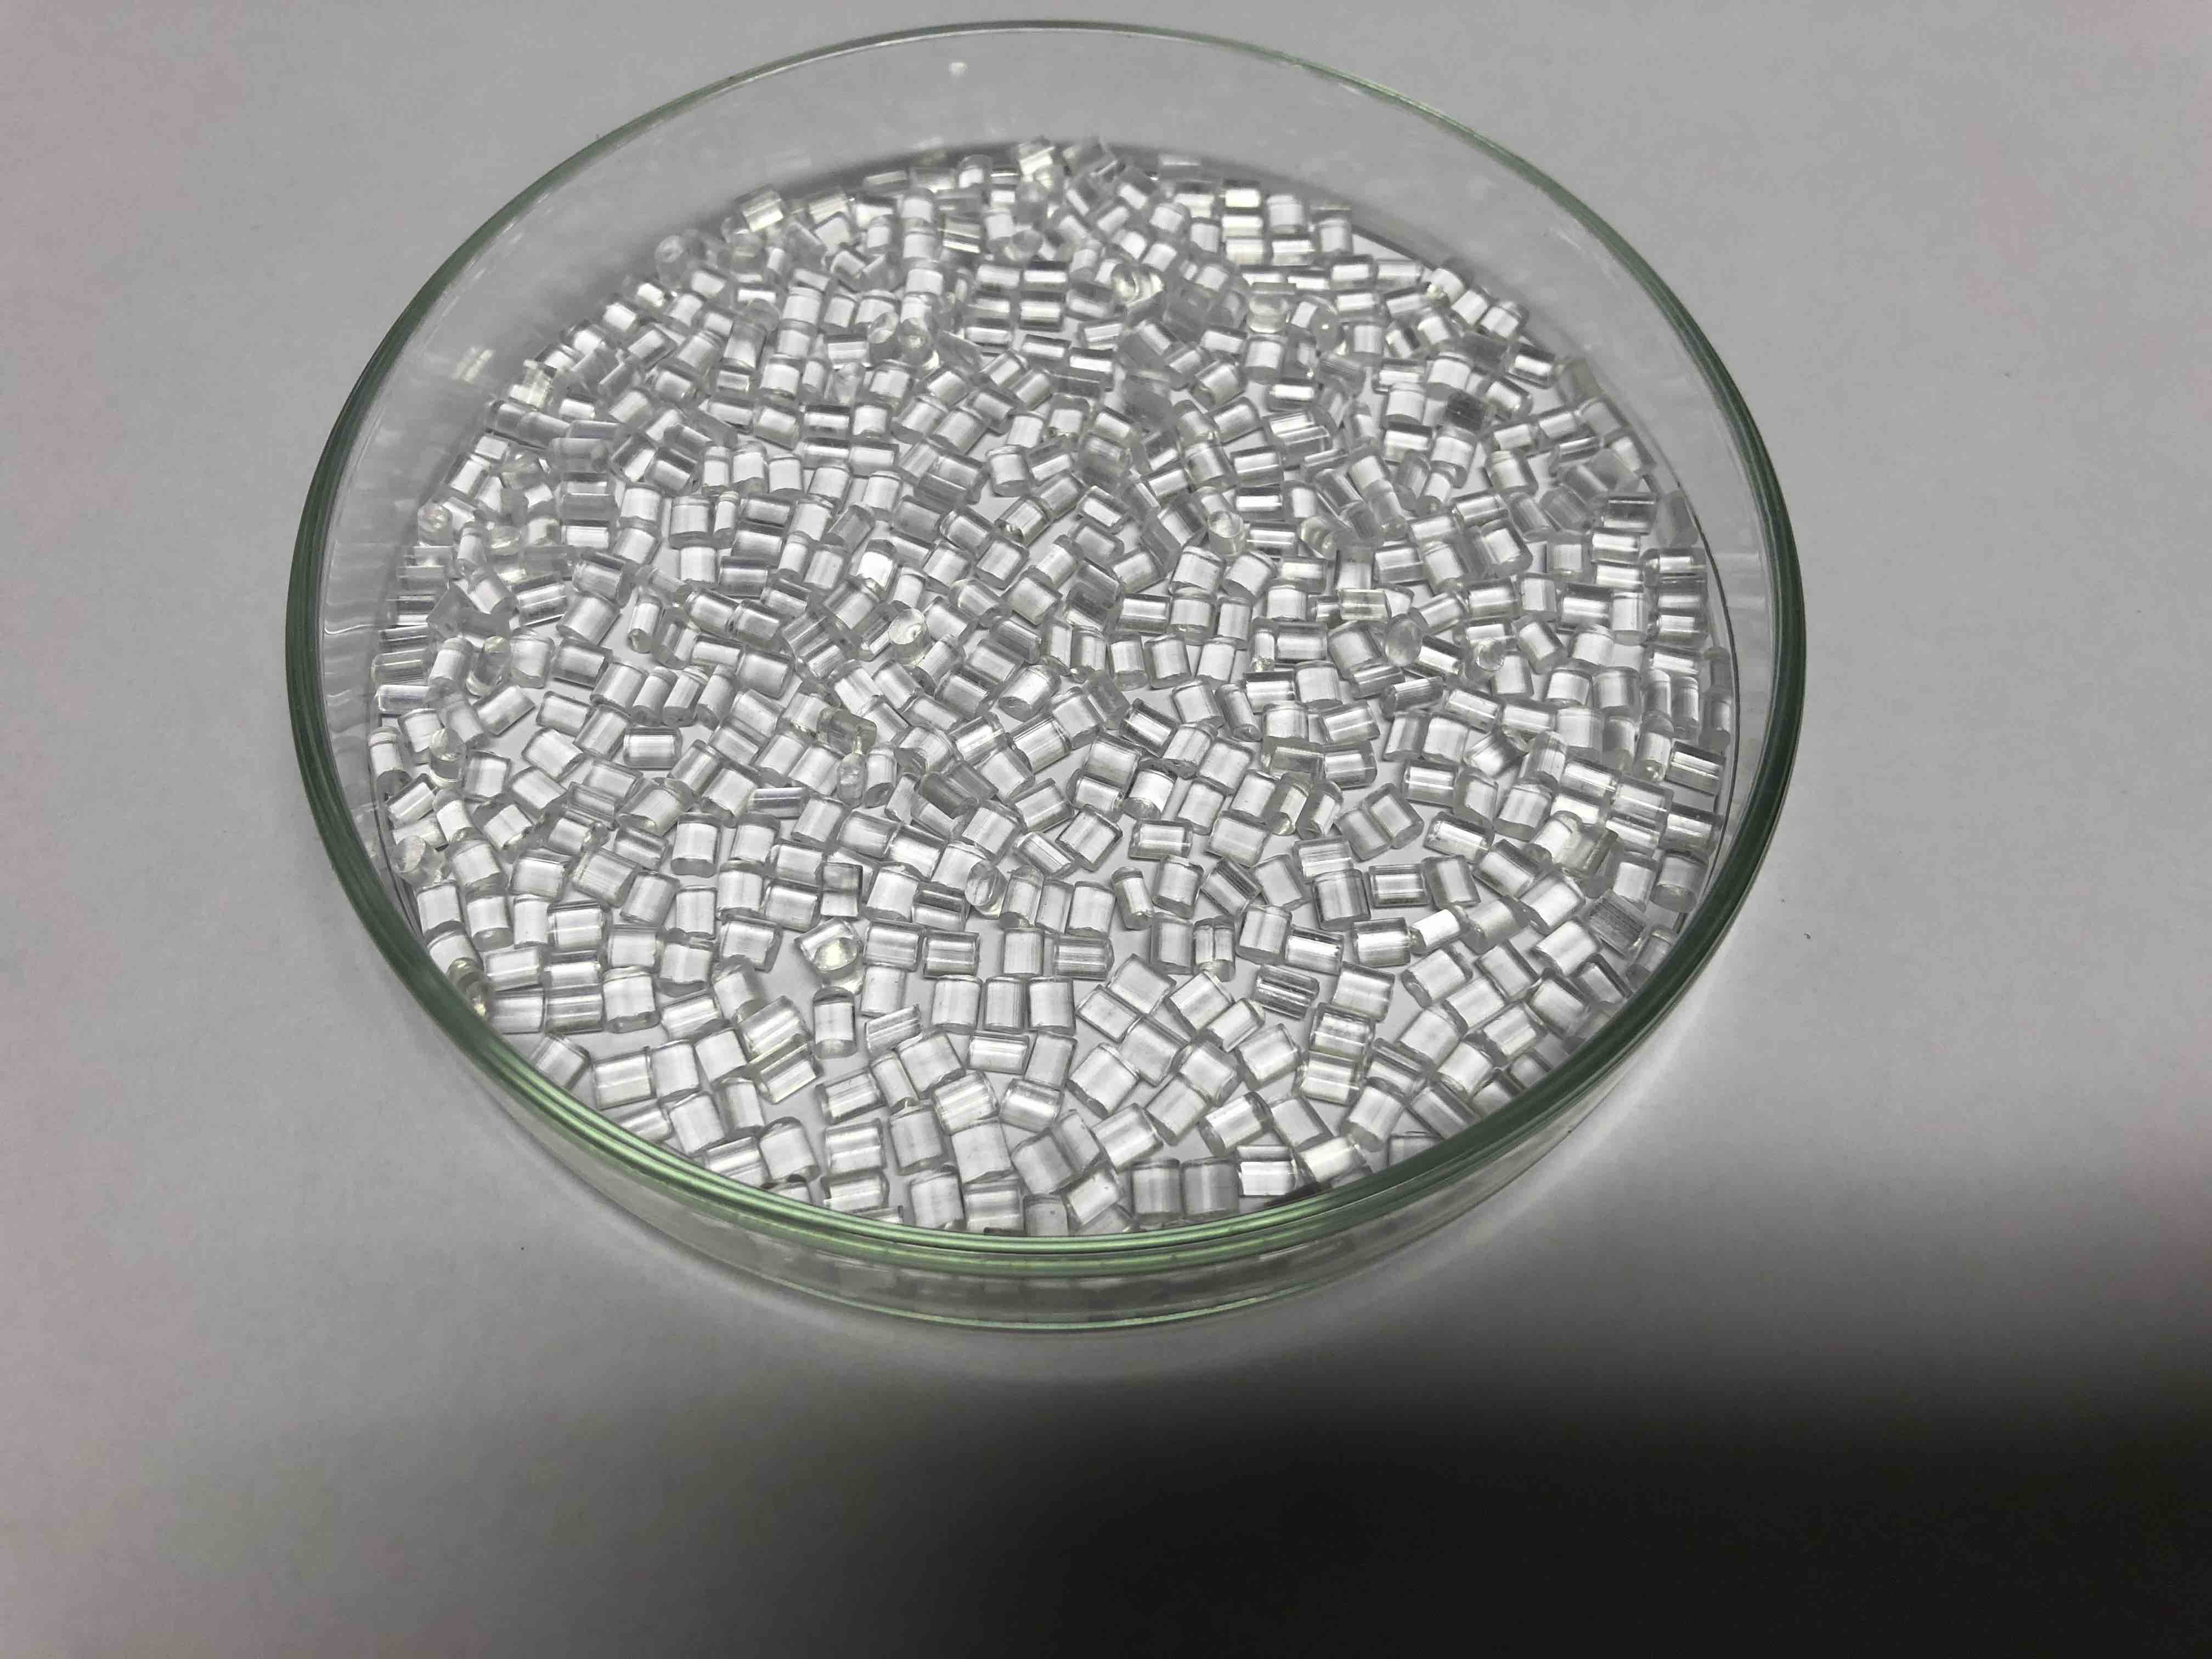
\includegraphics[width = 12cm]{Images/appendix/PET-pristine.jpg}
    \caption[$\; \:$PET Amorphous]{PET Amorphous, Clear}
    \label{fig:pet}
\end{figure}

\begin{figure}
    \centering
    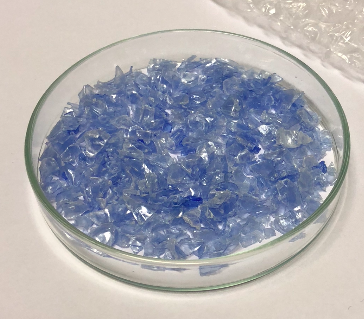
\includegraphics[width = 12cm]{Images/appendix/PET-pc.png}
    \caption[$\; \:$PET Post Consumer]{PET Post Consumer, Clear}
    \label{fig:pet-pc}
\end{figure}

\begin{figure}
    \centering
    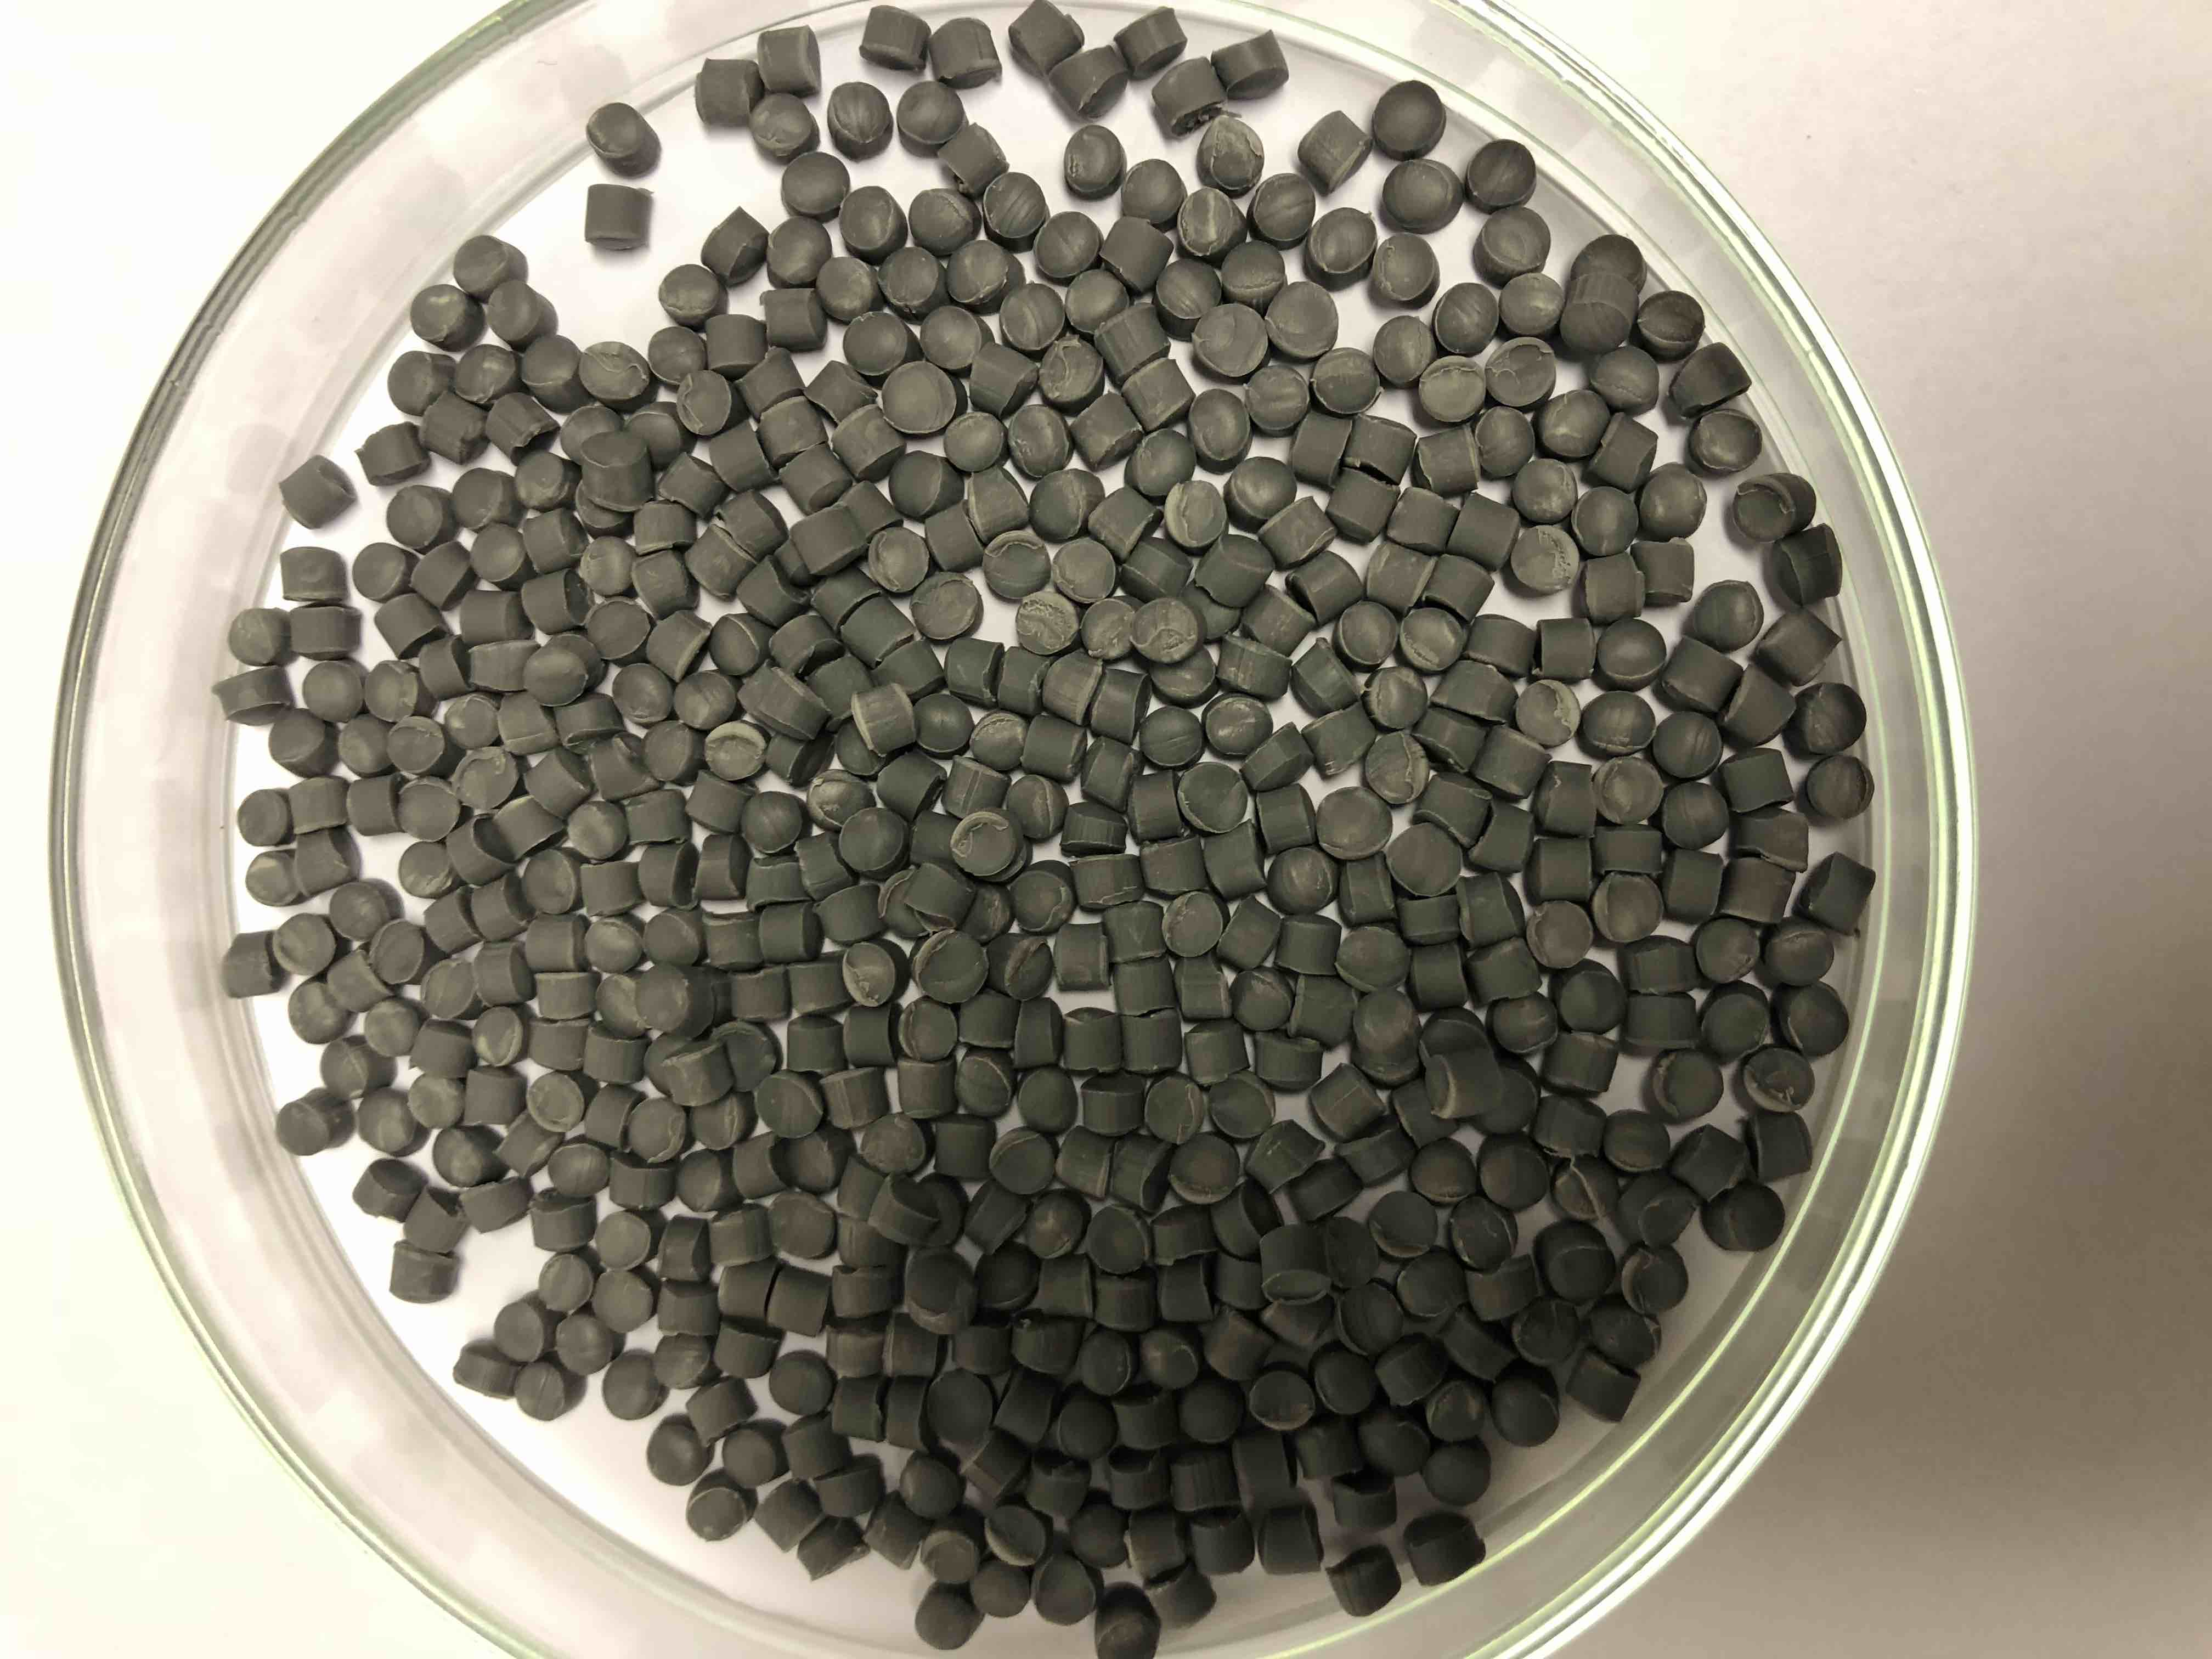
\includegraphics[width = 12cm]{Images/appendix/PP-recyclate-post-consumer.jpg}
    \caption[$\; \:$PP Post Consumer]{PP Post Consumer, Gray}
    \label{fig:pp-gray}
\end{figure}

\begin{figure}
    \centering
    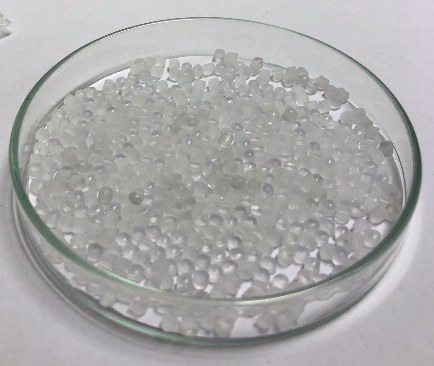
\includegraphics[width = 12cm]{Images/appendix/pp-pristine.png}
    \caption[$\; \:$PP Pristine]{PP Pristine, Clear}
    \label{fig:pp-clear}
\end{figure}

\begin{figure}
    \centering
    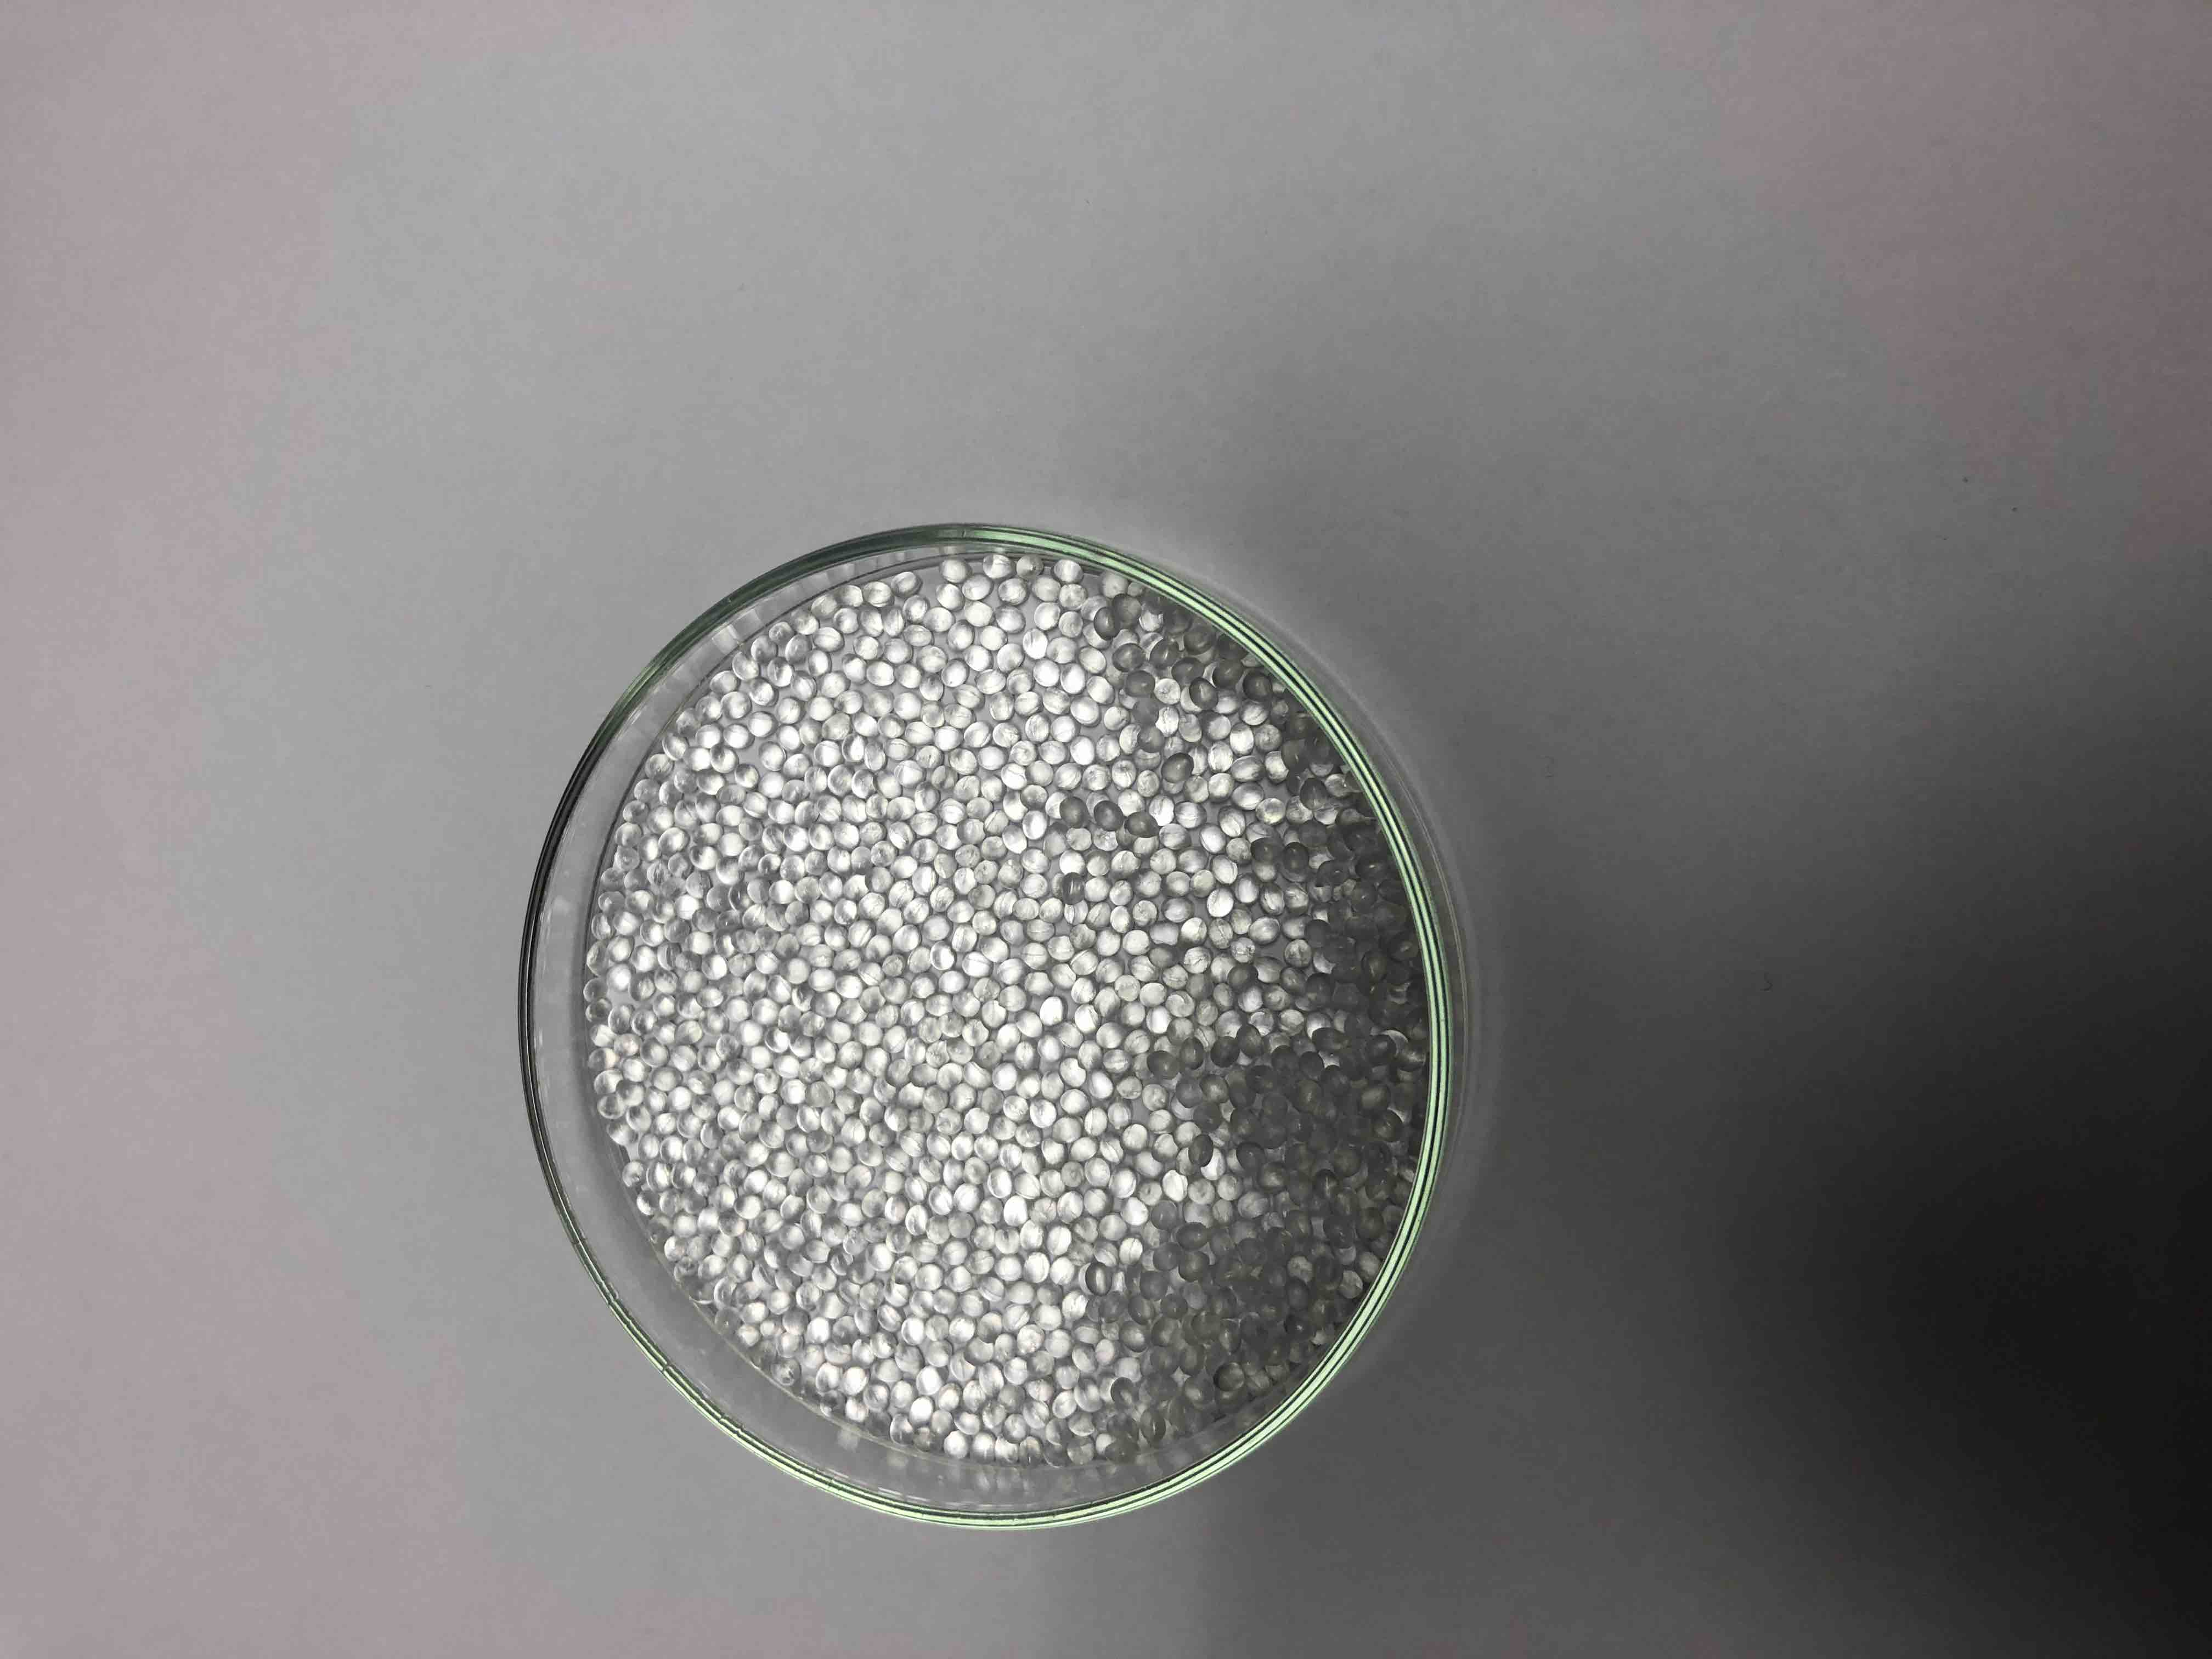
\includegraphics[width = 12cm]{Images/appendix/PS-pristine.jpg}
    \caption[$\; \:$PS Pristine]{PS Pristine, Clear}
    \label{fig:ps-clear}
\end{figure}

\begin{figure}
    \centering
    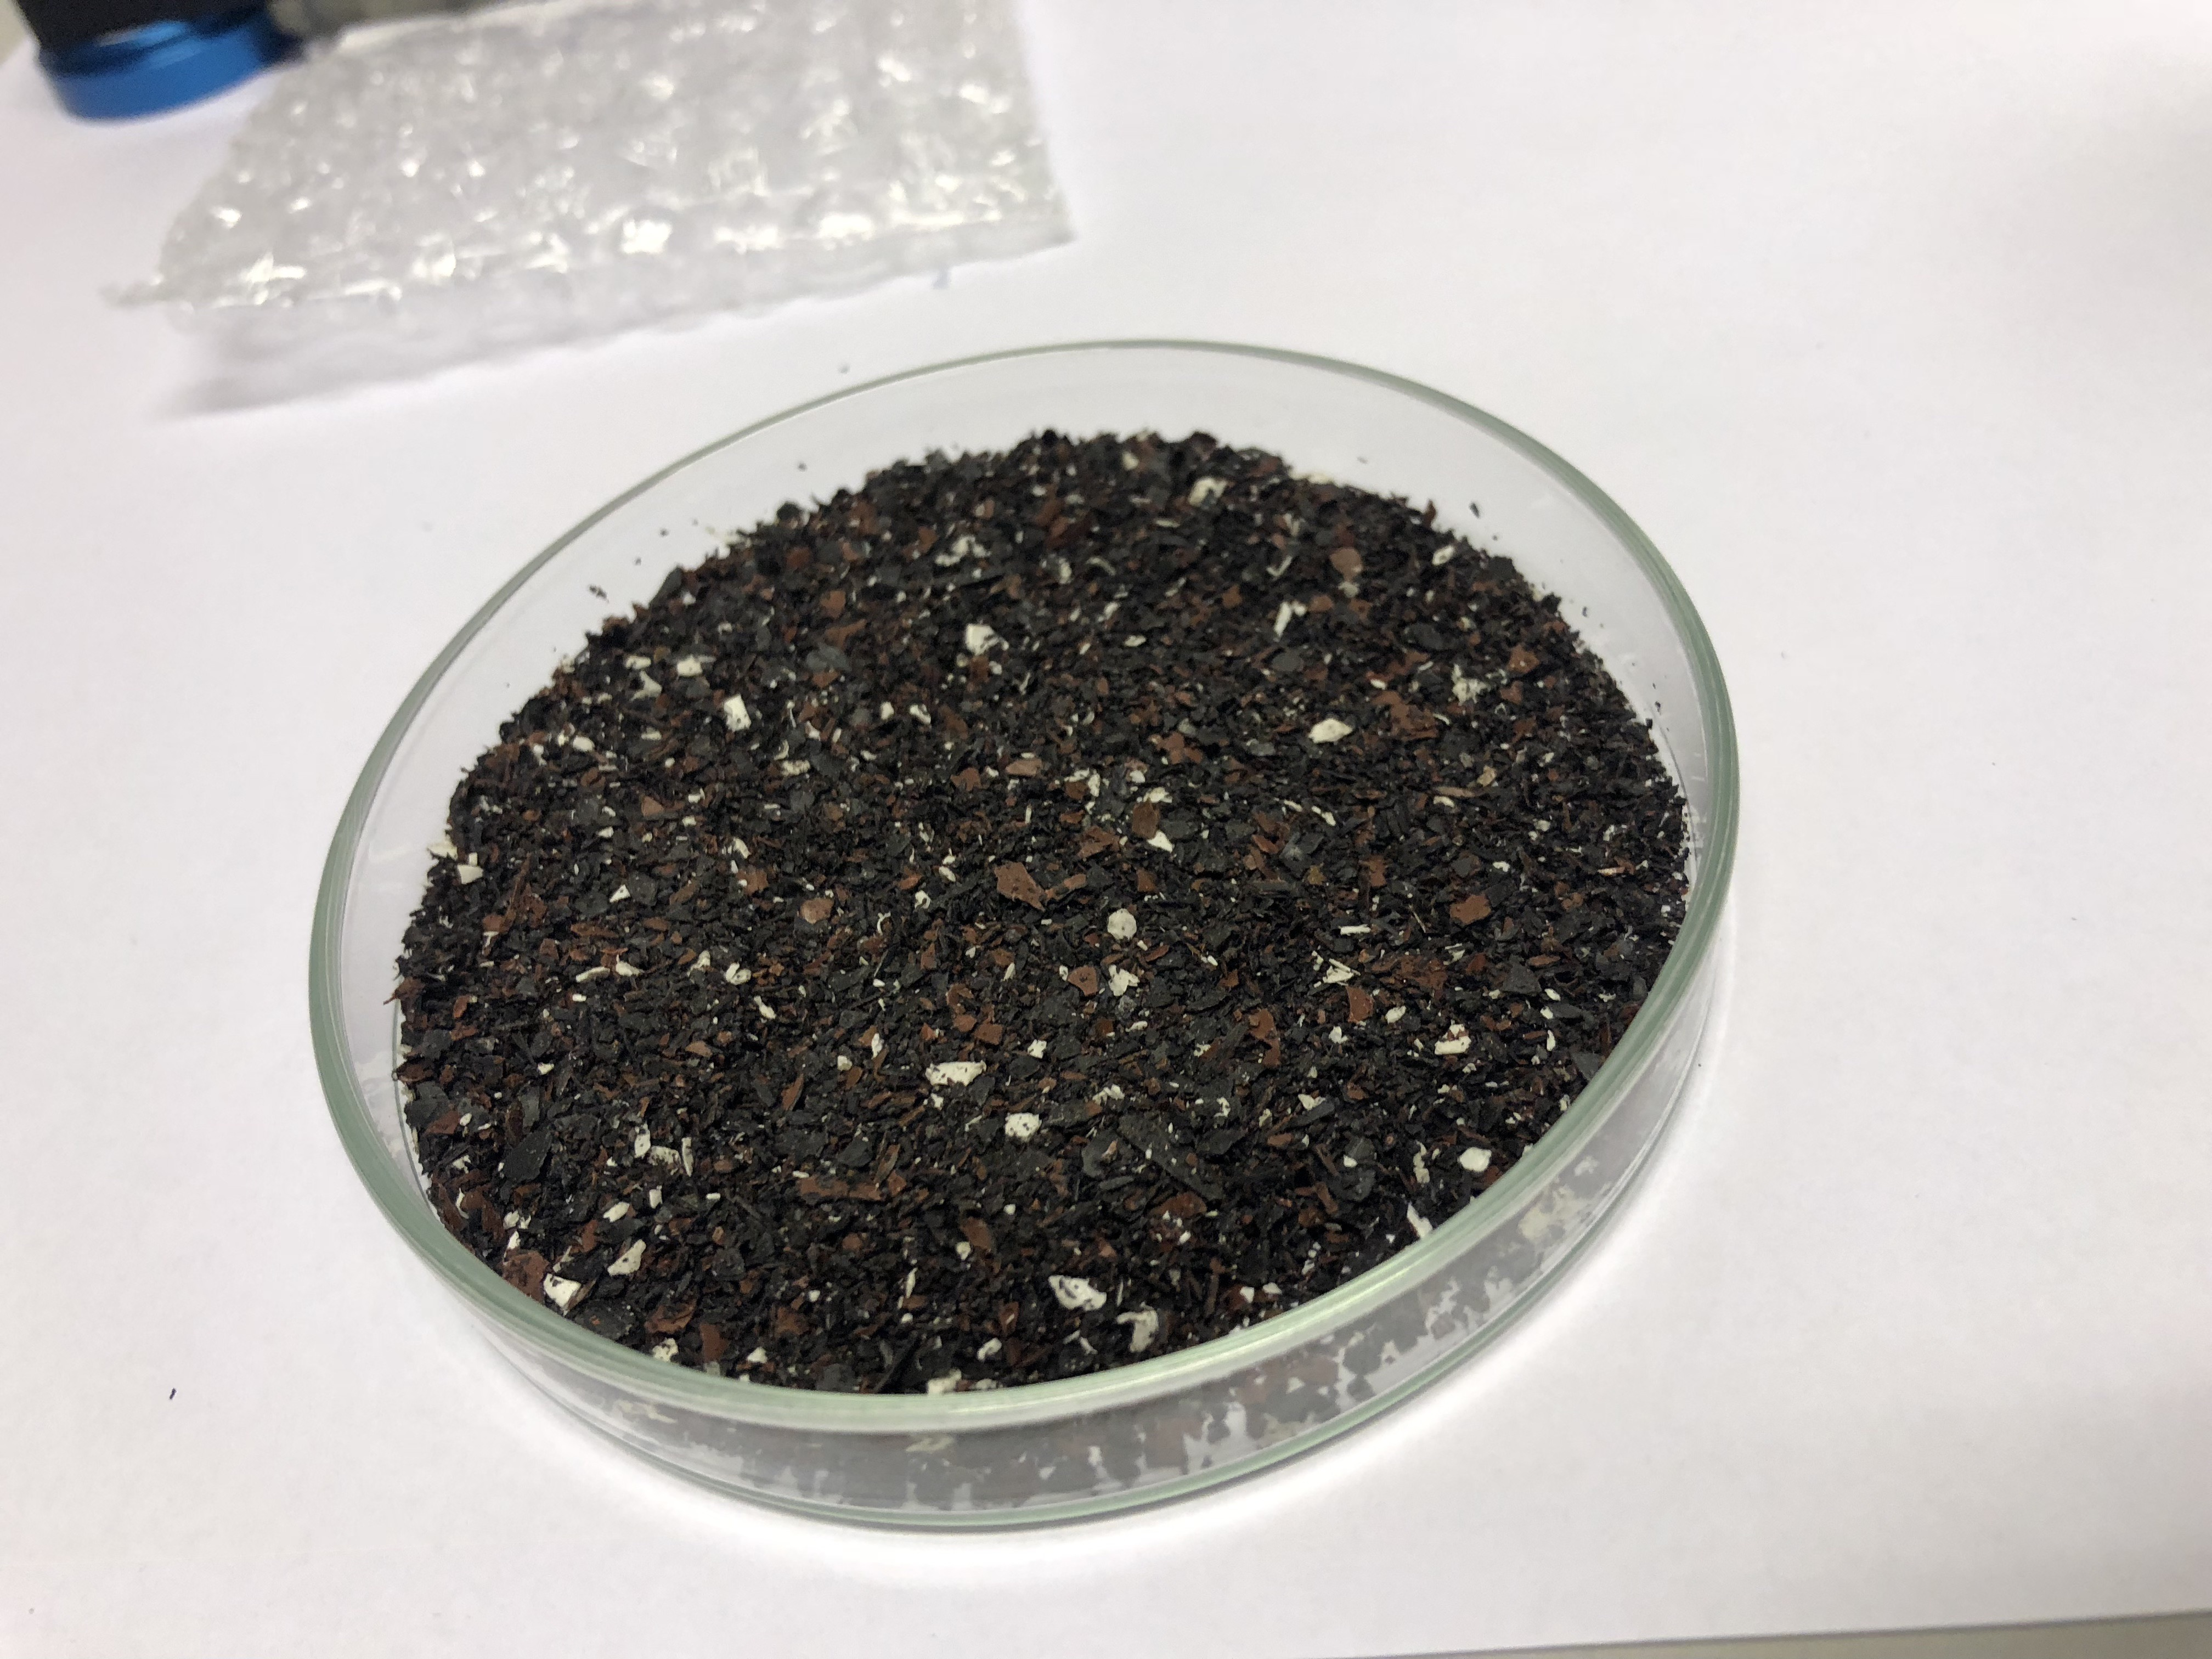
\includegraphics[width = 12cm]{Images/appendix/PS-Regrind-(Post-Industrial-Plant-Trays).jpg}
    \caption[$\; \:$PS Post Industrial]{PS Post Industrial, Looks like black/orange/white coffee powder}
    \label{fig:ps-coffee}
\end{figure}

\begin{figure}
    \centering
    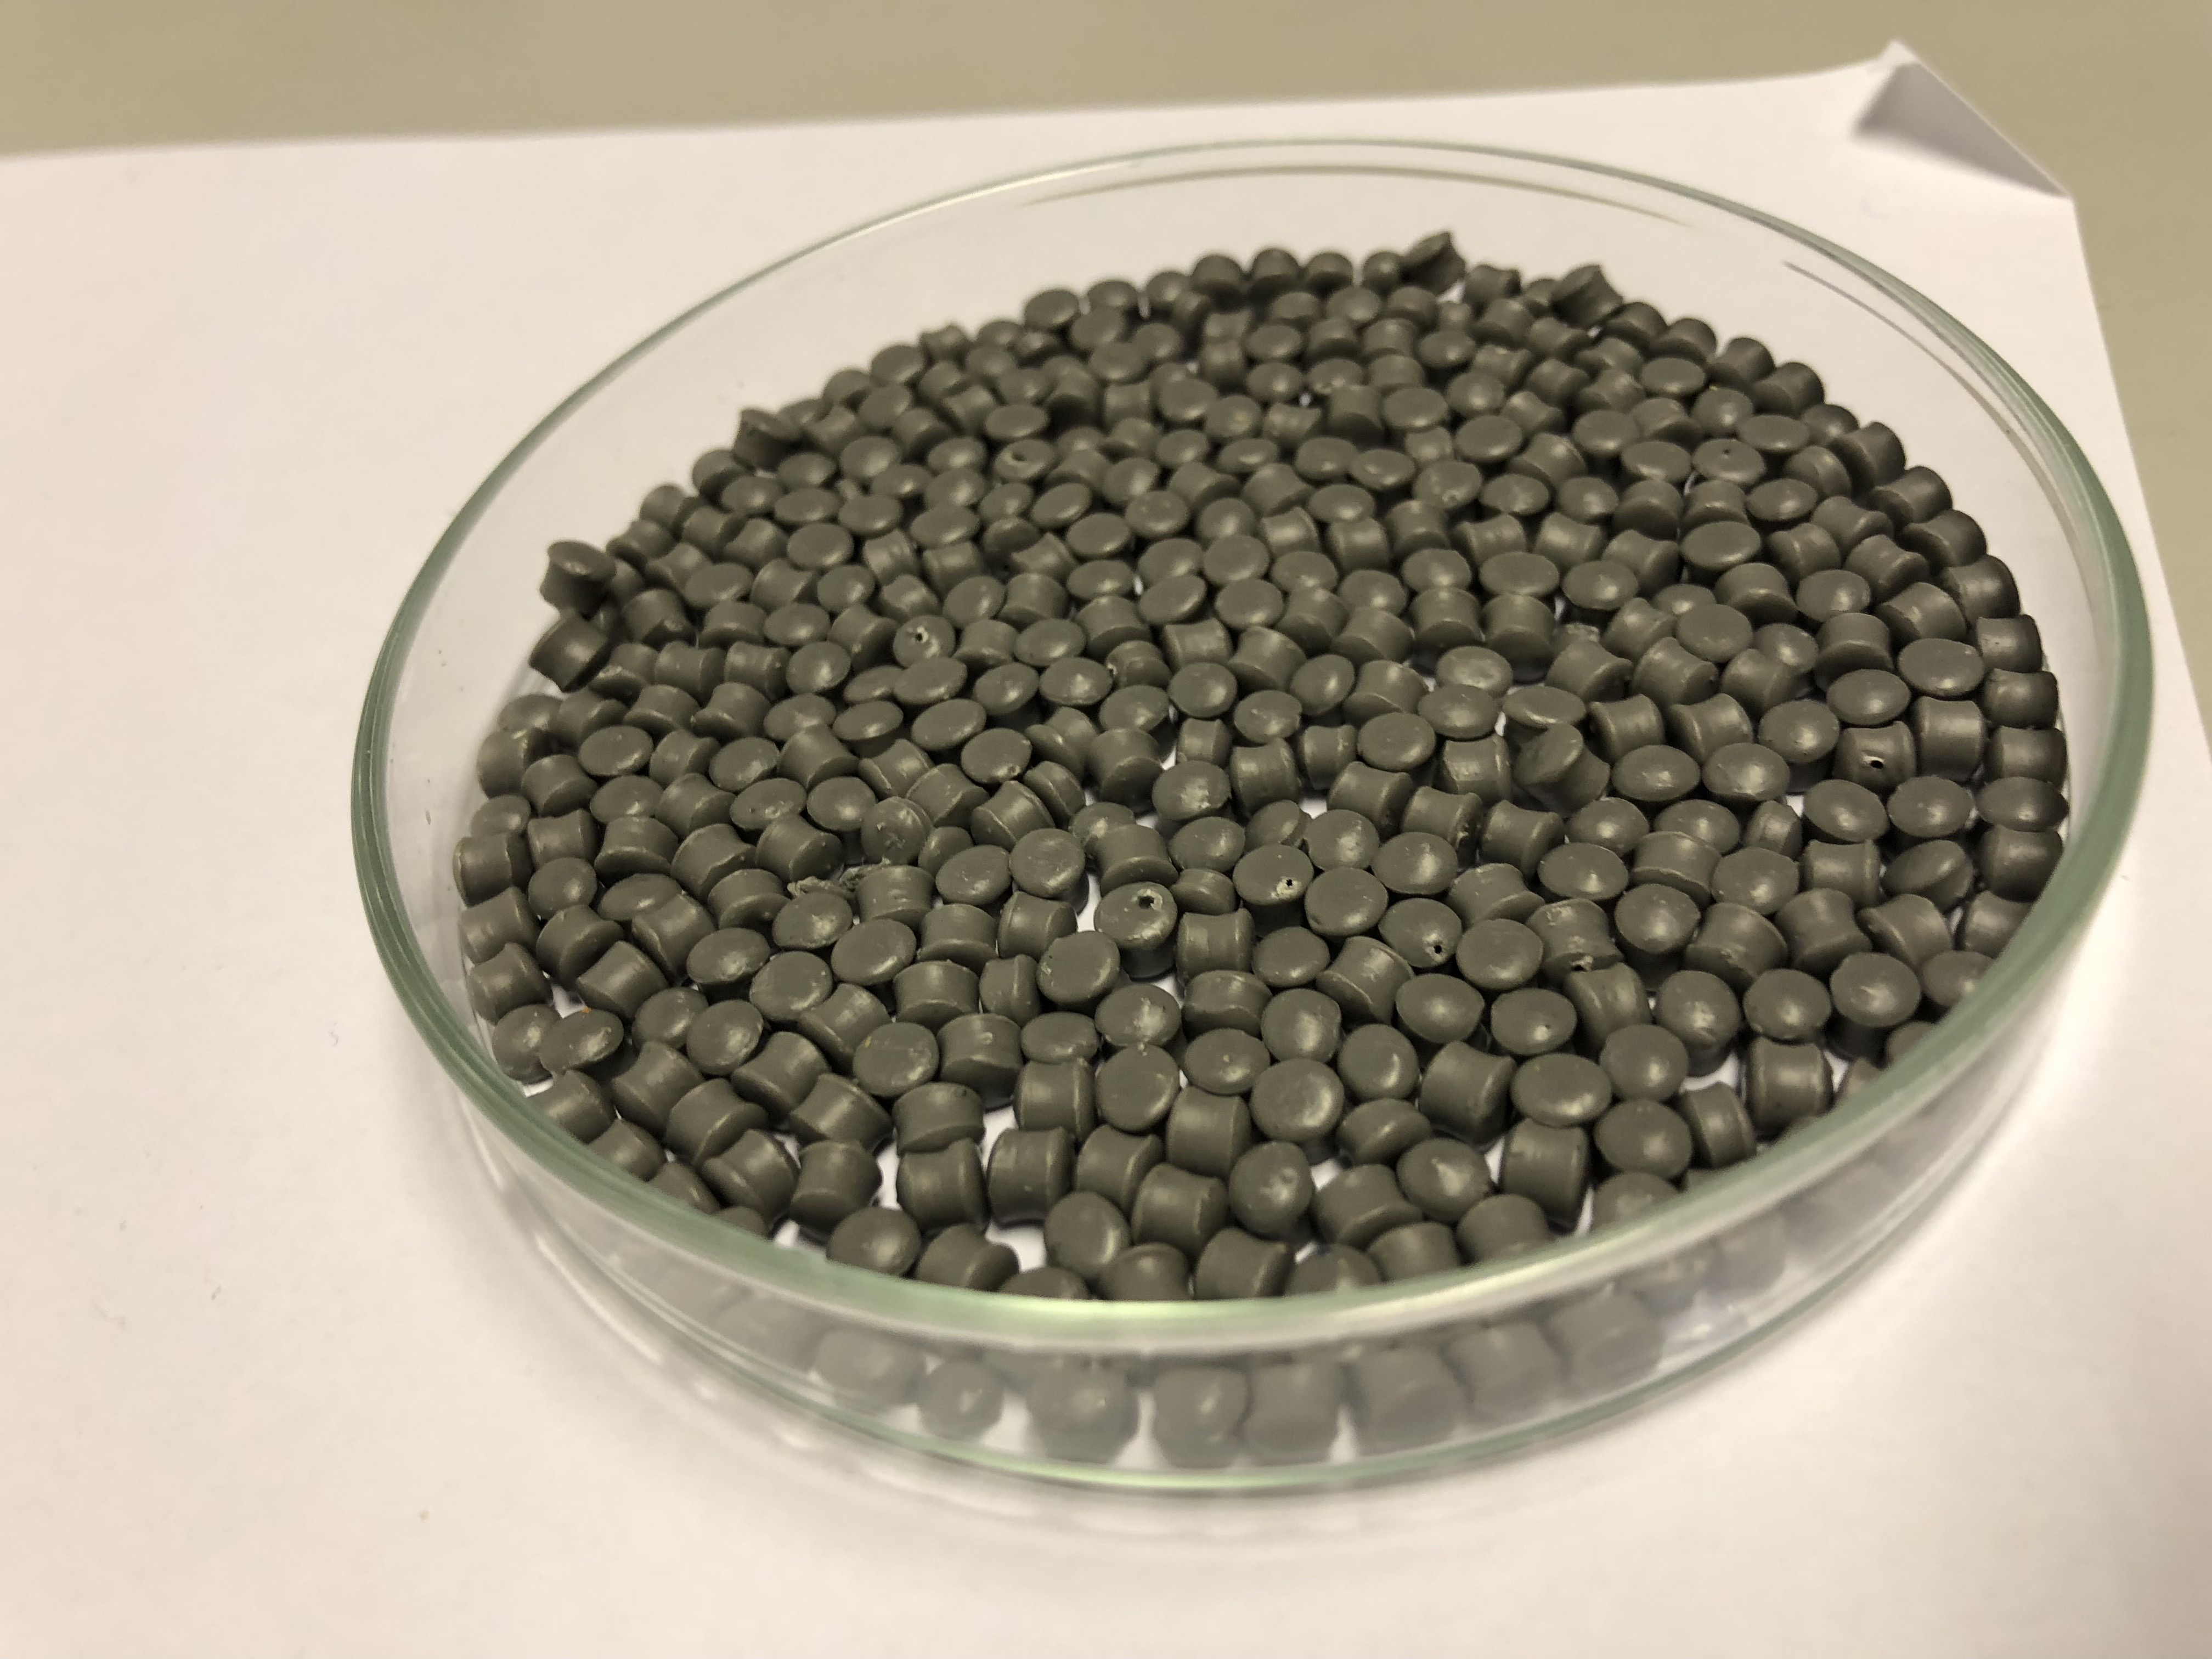
\includegraphics[width = 12cm]{Images/appendix/PVC-pristine.jpg}
    \caption[$\; \:$PVC Pristine]{PVC Pristine, Gray}
    \label{fig:pvc-gray}
\end{figure}

\begin{figure}
    \centering
    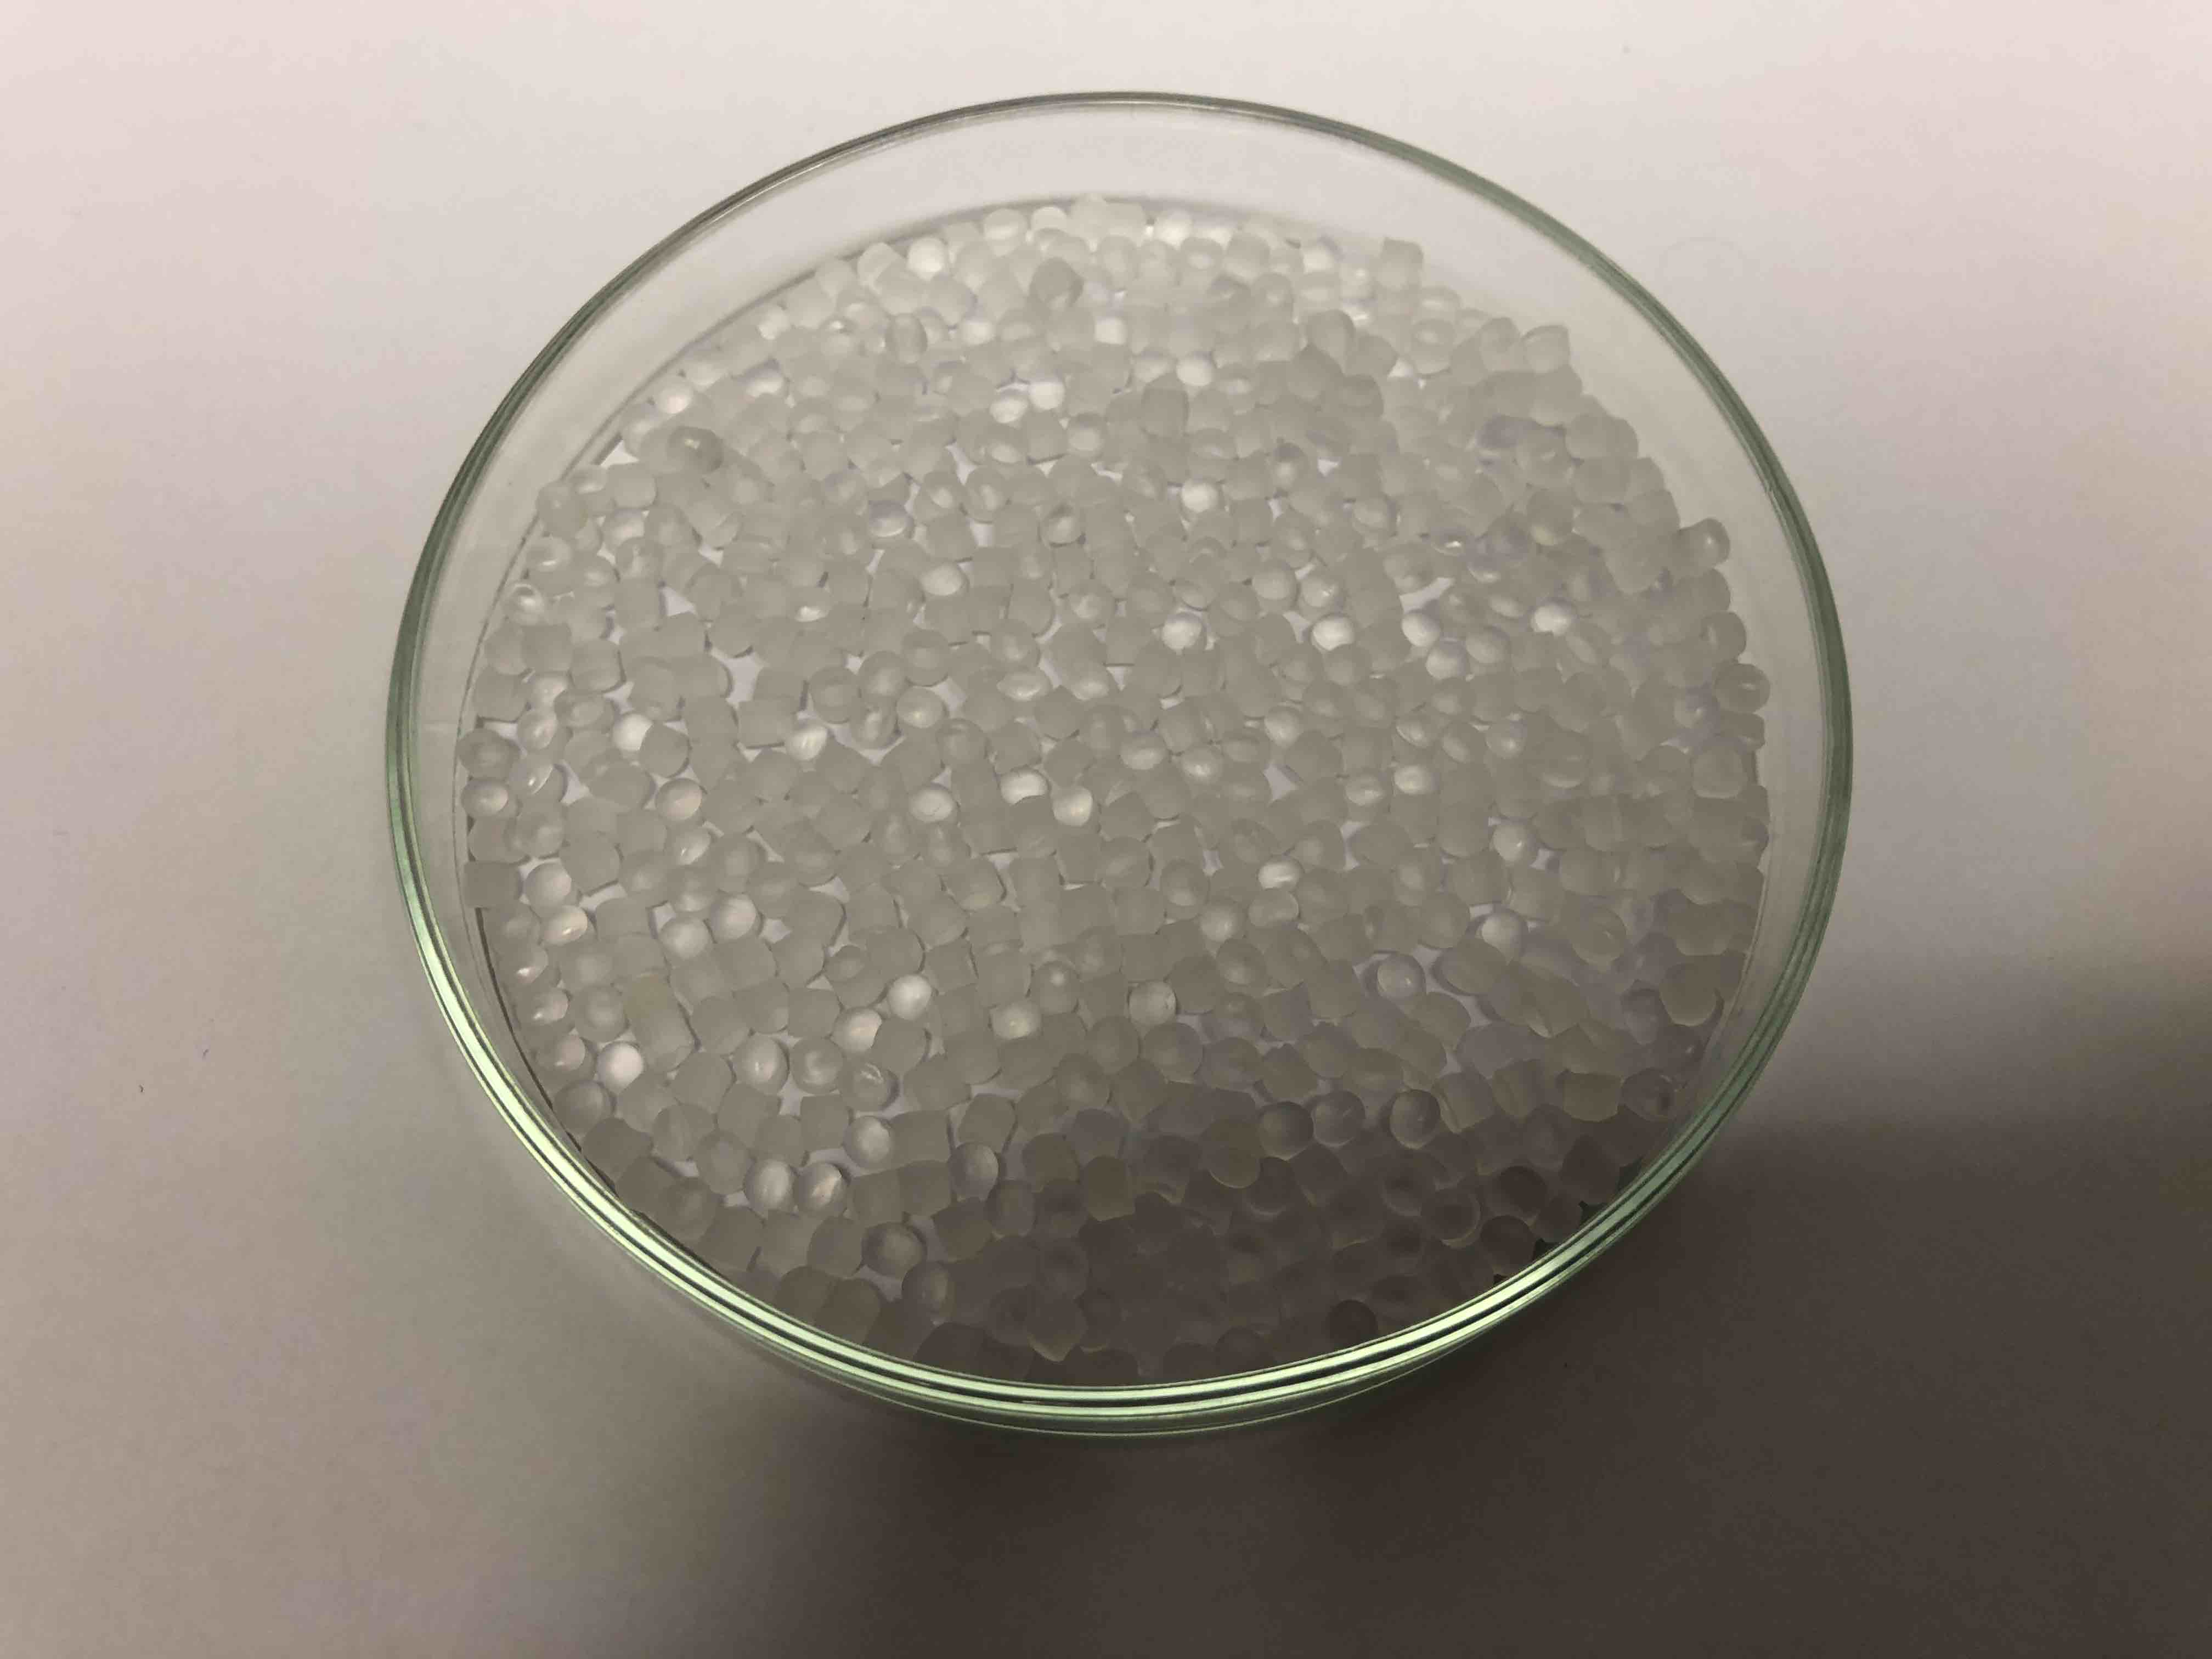
\includegraphics[width = 12cm]{Images/appendix/PVC-pristine-soft.jpg}
    \caption[$\; \:$PVC Soft]{PVC Soft, Pristine, Clear}
    \label{fig:pvc-clear}
\end{figure}

\begin{figure}
    \centering
    
\includegraphics[width = 6cm]{Images/appendix/remab.png}
    \caption[$\; \:$REMA Bag, Blue]{REMA Bag, Blue}
    \label{fig:remablue}
\end{figure}

\begin{figure}
    \centering
    
\includegraphics[width = 6cm]{Images/appendix/remar.png}
    \caption[$\; \:$REMA Bag, Red]{REMA Bag, Red}
    \label{fig:remared}
\end{figure}

\begin{figure}
    \centering
    
\includegraphics[width = 8cm]{Images/appendix/remaw.png}
    \caption[$\; \:$REMA Bag, White]{REMA Bag, White}
    \label{fig:remawhite}
\end{figure}

\begin{figure}
    \centering
    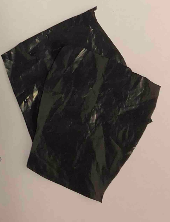
\includegraphics[width = 5cm]{Images/appendix/vmp.png}
    \caption[$\; \:$Vinmonopolet Bag]{Vinmonopolet Bag, Black}
    \label{fig:vinmono}
\end{figure}

















\chapter{Plots of Signatures}
\label{app:signatures}

\begin{figure}
    \centering
    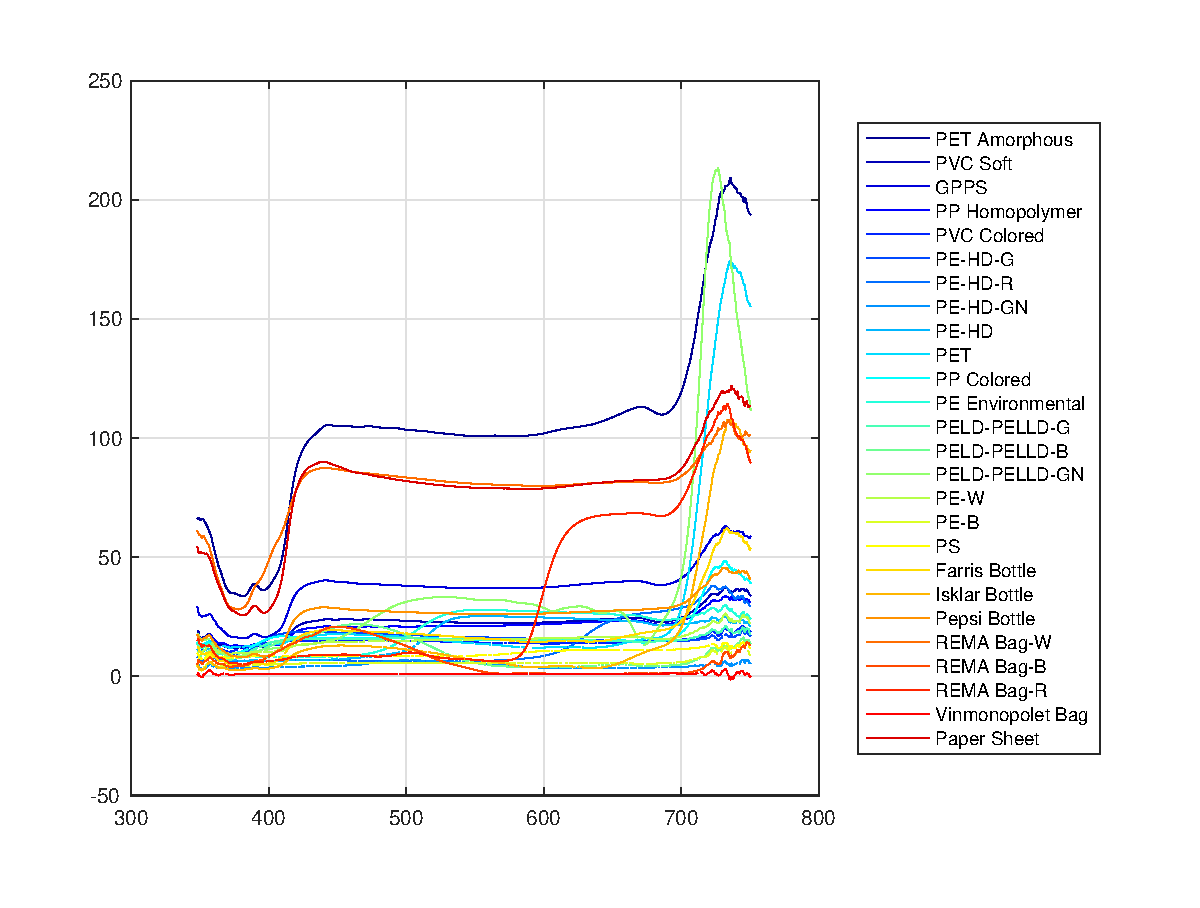
\includegraphics[width = 12cm]{Images/appendix/All.eps}
    \caption{All plastic types}
    \label{fig:all}
\end{figure}

\begin{figure}
    \centering
    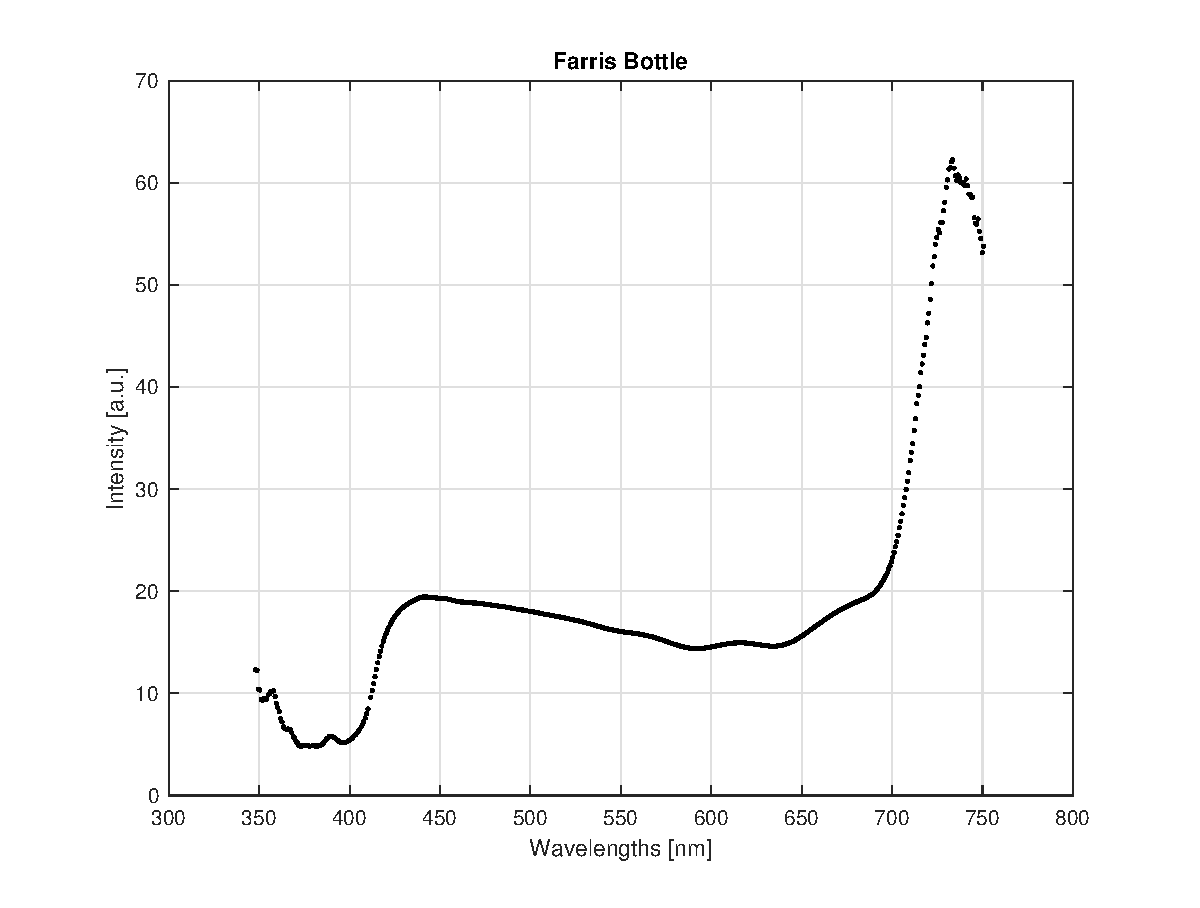
\includegraphics[width = 12cm]{Images/appendix/farris.eps}
    \caption{Farris}
    \label{fig:my_label}
\end{figure}

\begin{figure}
    \centering
    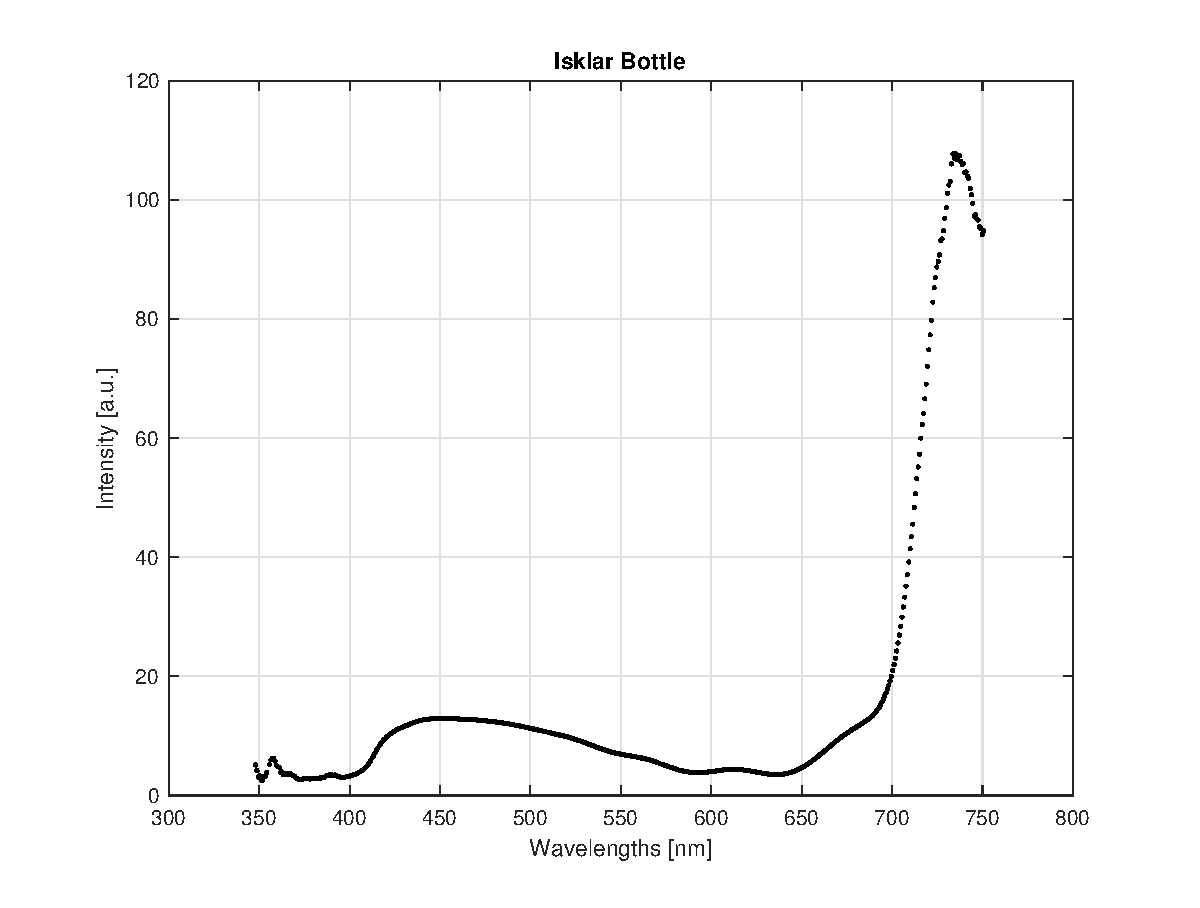
\includegraphics[width = 12cm]{Images/appendix/isklar_blue.eps}
    \caption{Isklar, Blue}
    \label{fig:isklar}
\end{figure}

\begin{figure}
    \centering
    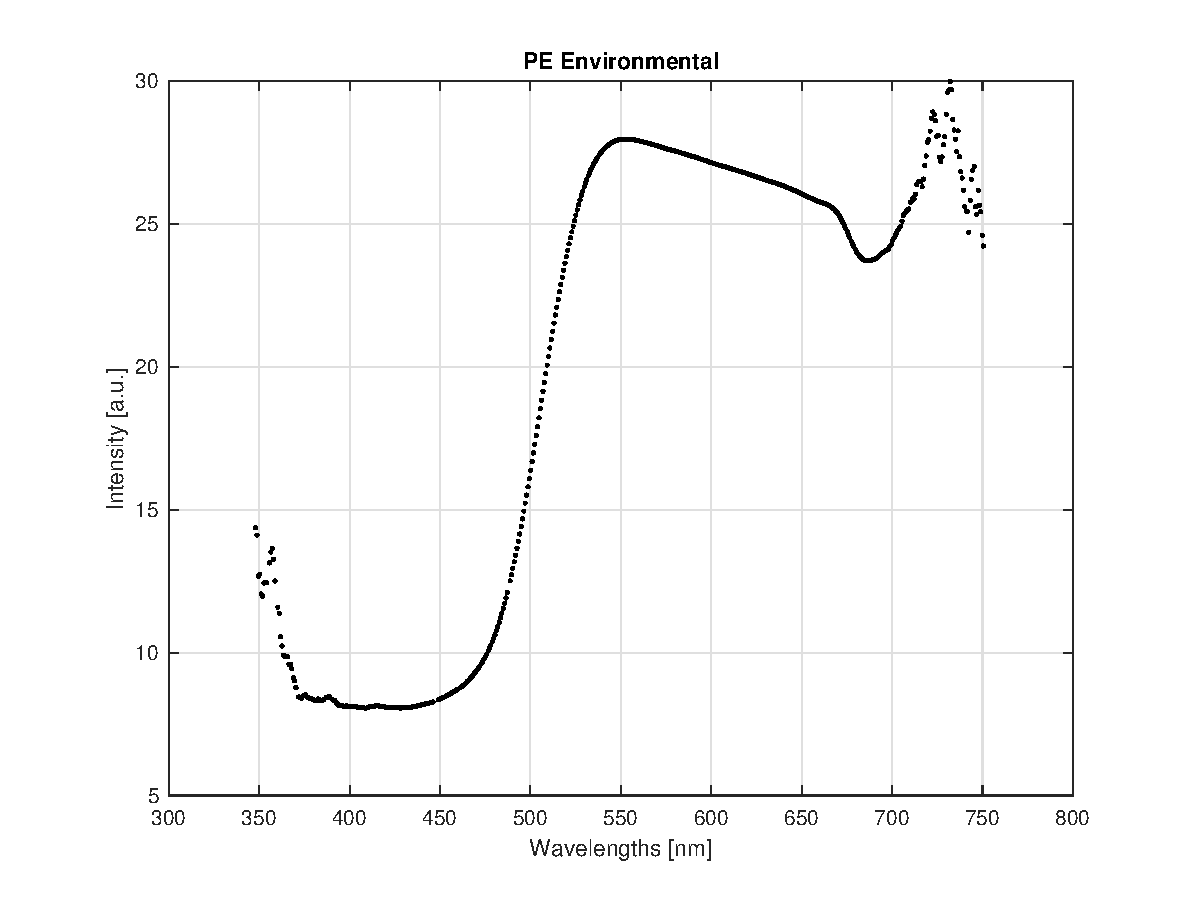
\includegraphics[width = 12cm]{Images/appendix/p-env_yellowbowl.eps}
    \caption{PE environmental (yellow fishbowl)}
    \label{fig:pe_env}
\end{figure}

\begin{figure}
    \centering
    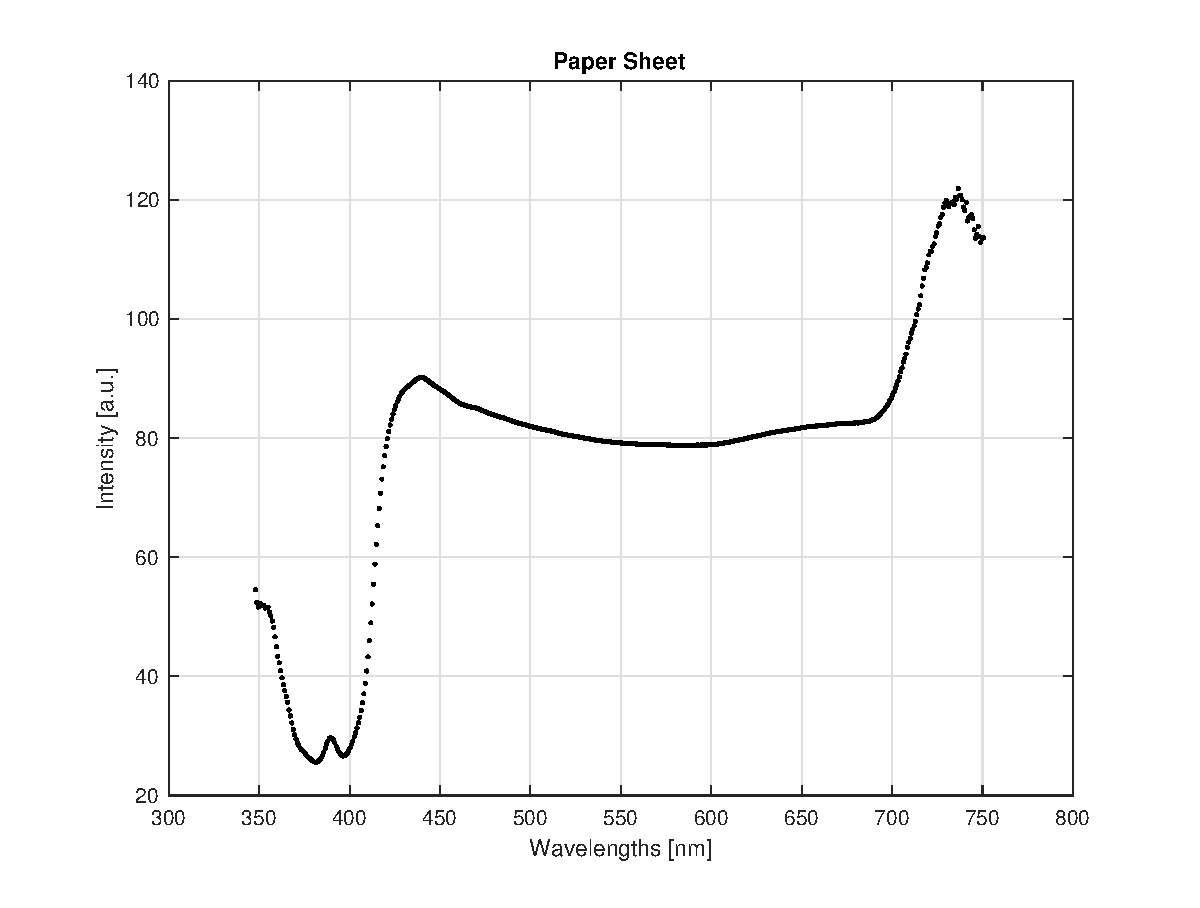
\includegraphics[width = 12cm]{Images/appendix/papersheet.eps}
    \caption{Paper sheet}
    \label{fig:paper}
\end{figure}

\begin{figure}
    \centering
    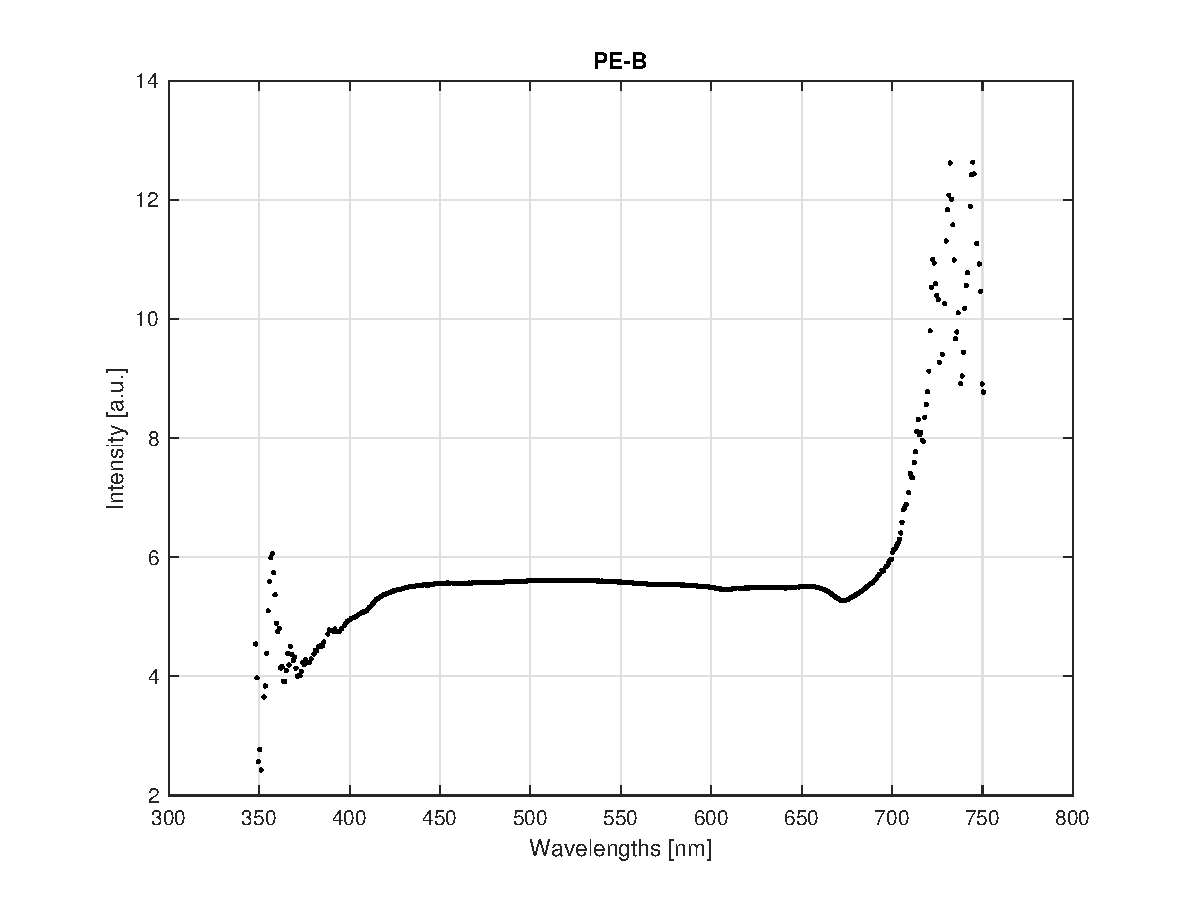
\includegraphics[width = 12cm]{Images/appendix/pe-beach-black.eps}
    \caption{PE beach-pellets, black}
    \label{fig:pe_beach_b}
\end{figure}

\begin{figure}
    \centering
    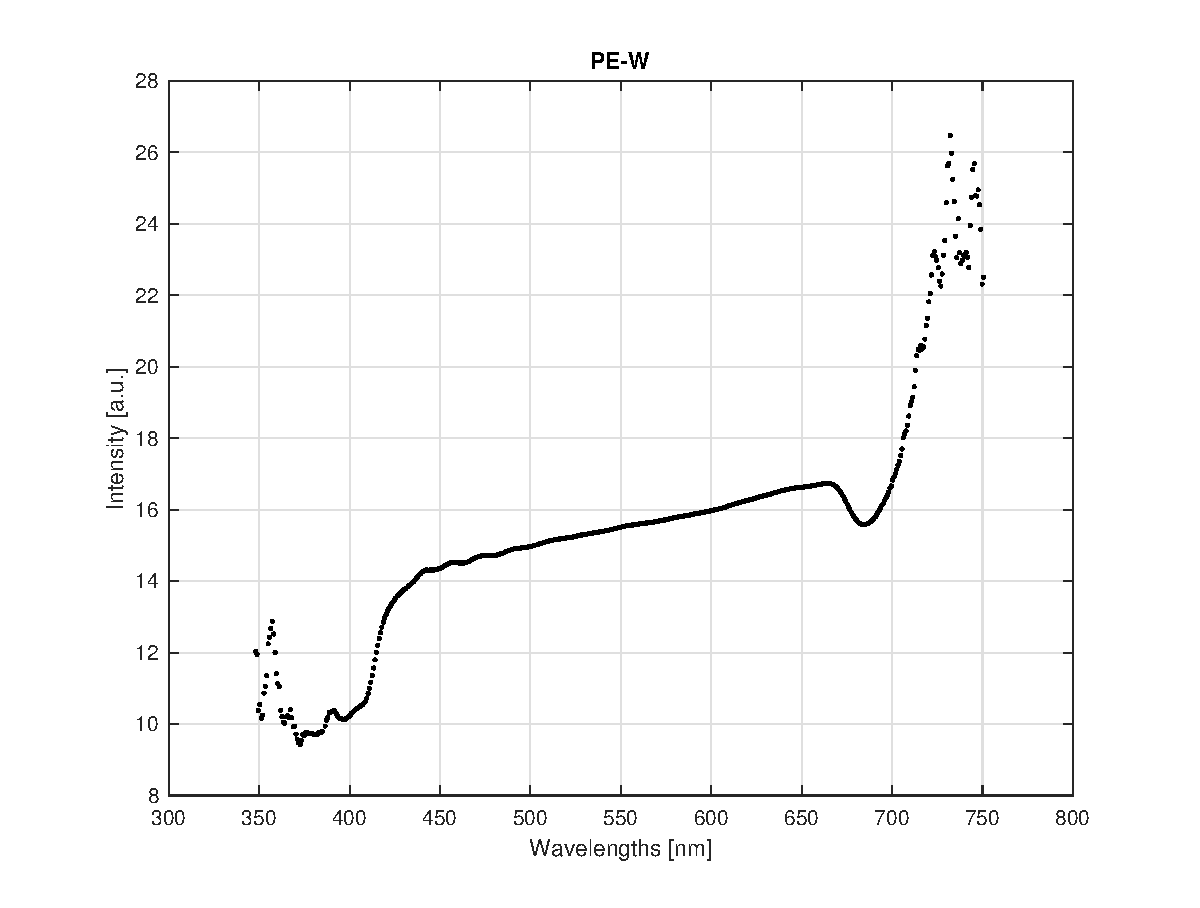
\includegraphics[width = 12cm]{Images/appendix/pe-beach-white.eps}
    \caption{PE beach-pellets, white}
    \label{fig:pe_beach_w}
\end{figure}

\begin{figure}
    \centering
    \includegraphics[width = 12cm]{Images/appendix/pe-hd-postconsum-gray.eps}
    \caption{PE-HD Post Consumer, Gray}
    \label{fig:pehd-gray}
\end{figure}

\begin{figure}
    \centering
    \includegraphics[width = 12cm]{Images/appendix/pe-hd-postconsum-red.eps}
    \caption{PE-HD Post Consumer, Red}
    \label{fig:pehd-red}
\end{figure}

\begin{figure}
    \centering
    \includegraphics[width = 12cm]{Images/appendix/pe-hd-postconsum.eps}
    \caption[$\; \:$PE-HD Post Consumer, Yellow]{PE-HD Post Consumer, Yellow}
    \label{fig:pehd-yellow}
\end{figure}

\begin{figure}
    \centering
    \includegraphics[width = 12cm]{Images/appendix/pe-hd-postconsumer-green.eps}
    \caption[$\; \:$PE-HD Post Consumer, Green]{PE-HD, Post Consumer, Green}
    \label{fig:pehd-green}
\end{figure}

\begin{figure}
    \centering
    \includegraphics[width = 12cm]{Images/appendix/pe-ld-postindust-blue.eps}
    \caption[$\; \:$PE-LD Post Industrial, Blue]{PE-LD, Post Industrial, Blue}
    \label{fig:peld-blue}
\end{figure}

\begin{figure}
    \centering
    \includegraphics[width = 12cm]{Images/appendix/pe-ld-postindust-gray.eps}
    \caption[$\; \:$PE-LD Post Industrial, Gray]{PE-LD, Post Industrial, Gray}
    \label{fig:peld-gray}
\end{figure}

\begin{figure}
    \centering
    \includegraphics[width = 12cm]{Images/appendix/pe-ld-postindust-green.eps}
    \caption[$\; \:$PE-LD Post Industrial, Green]{PE-LD Post Industrial, Green}
    \label{fig:peld-green}
\end{figure}

\begin{figure}
    \centering
    \includegraphics[width = 12cm]{Images/appendix/pepsi.eps}
    \caption[$\; \:$Pepsi]{Pepsi}
    \label{fig:pepsi}
\end{figure}

\begin{figure}
    \centering
    \includegraphics[width = 12cm]{Images/appendix/pet-amorphous-pristine-clear.eps}
    \caption[$\; \:$PET Amorphous]{PET Amorphous, Clear}
    \label{fig:pet}
\end{figure}

\begin{figure}
    \centering
    \includegraphics[width = 12cm]{Images/appendix/pet-postconsum.eps}
    \caption[$\; \:$PET Post Consumer]{PET Post Consumer, Clear}
    \label{fig:pet-pc}
\end{figure}

\begin{figure}
    \centering
    \includegraphics[width = 12cm]{Images/appendix/pp-postconsum-gray.eps}
    \caption[$\; \:$PP Post Consumer]{PP Post Consumer, Gray}
    \label{fig:pp-gray}
\end{figure}

\begin{figure}
    \centering
    \includegraphics[width = 12cm]{Images/appendix/pp-pristine-clear.eps}
    \caption[$\; \:$PP Pristine]{PP Pristine, Clear}
    \label{fig:pp-clear}
\end{figure}

\begin{figure}
    \centering
    \includegraphics[width = 12cm]{Images/appendix/ps-pristine-clear.eps}
    \caption[$\; \:$PS Pristine]{PS Pristine, Clear}
    \label{fig:ps-clear}
\end{figure}

\begin{figure}
    \centering
    \includegraphics[width = 12cm]{Images/appendix/ps-postindust.eps}
    \caption[$\; \:$PS Post Industrial]{PS Post Industrial, Looks like black/orange/white coffee powder}
    \label{fig:ps-coffee}
\end{figure}

\begin{figure}
    \centering
    \includegraphics[width = 12cm]{Images/appendix/pvc-pristine-colored.eps}
    \caption[$\; \:$PVC Pristine]{PVC Pristine, Gray}
    \label{fig:pvc-gray}
\end{figure}

\begin{figure}
    \centering
    \includegraphics[width = 12cm]{Images/appendix/pvc-soft-pristine-clear.eps}
    \caption[$\; \:$PVC Soft]{PVC Soft, Pristine, Clear}
    \label{fig:pvc-clear}
\end{figure}

\begin{figure}
    \centering
    \includegraphics[width = 12cm]{Images/appendix/remablue.eps}
    \caption[$\; \:$REMA Bag, Blue]{REMA Bag, Blue}
    \label{fig:remablue}
\end{figure}

\begin{figure}
    \centering
    \includegraphics[width = 12cm]{Images/appendix/remared.eps}
    \caption[$\; \:$REMA Bag, Red]{REMA Bag, Red}
    \label{fig:remared}
\end{figure}

\begin{figure}
    \centering
    \includegraphics[width = 12cm]{Images/appendix/remawhite.eps}
    \caption[$\; \:$REMA Bag, White]{REMA Bag, White}
    \label{fig:remawhite}
\end{figure}

\begin{figure}
    \centering
    \includegraphics[width = 12cm]{Images/appendix/vinmono.eps}
    \caption[$\; \:$Vinmonopolet Bag]{Vinmonopolet Bag, Black}
    \label{fig:vinmono}
\end{figure}





\end{appendices}




